% Author = Thomas Liam Hilder
% Date   = 20/09/2022

% Setup
\documentclass[11pt,a4paper,onecolumn]{report}

\usepackage[margin=20mm]{geometry}


% Packages
\usepackage[T1]{fontenc} %Allows more exotic characters to be displayed properly (eg, Đ)
\usepackage{lmodern} %Makes T1 not ugly on a PDF viewer.
\usepackage[utf8]{inputenc}
\usepackage{amsmath}
\usepackage{amssymb}
\usepackage{graphicx}
\usepackage{float}
\usepackage{esint}
\usepackage{natbib}
\usepackage{hyperref}
\usepackage{xcolor}
\usepackage{cancel}
\usepackage{fancyhdr}
\usepackage{tocbibind}
\usepackage{enumitem}

\settocbibname{References}

\pagestyle{fancy}
\cfoot{\thepage}
\lhead[\leftmark]{}
\rhead[]{\leftmark}

 % customise hyperlinks
\hypersetup{allbordercolors=.9 .9 .9}

% custom commands
\renewcommand{\floatpagefraction}{.8}
\newcommand{\fct}{\textcolor{purple}{CITATIONS }}
\newcommand{\feqr}{\textcolor{purple}{EQ\_REF }}
\newcommand{\note}[1]{\textcolor{red}{Note: #1}}
\newcommand{\pderiv}[2]{\left(\frac{\partial #1}{\partial #2}\right)}
\newcommand{\VF}[1]{\mathbf{#1}}
\newcommand{\dif}{\mathop{}\!\mathrm{d}}
\newcommand{\appropto}{\mathrel{\vcenter{
  \offinterlineskip\halign{\hfil$##$\cr
    \propto\cr\noalign{\kern2pt}\sim\cr\noalign{\kern-2pt}}}}}

% Details
\title{Measuring Young Planets from their Spiral Wakes}
\author{Thomas Hilder}
\date{September 2022}

% Document
\begin{document}
    
    % TITLE PAGE
    \begin{titlepage}
    \begin{center}
        \par\noindent\rule{\textwidth}{0.8pt}
       
        \vspace*{1cm}

        \makeatletter
        {\LARGE\textbf{\@title}}

        \vspace{0.5cm}

        \textsc{Honours Thesis}

        \vspace{0.4cm}

        \par\noindent\rule{\textwidth}{0.8pt}
       
        \vspace{0.9cm}

        {\Large\textbf{by \@author}} \\
        \makeatother
        
        \vspace{0.75cm}
        
        {\large\textit{Supervisors:} \\ Daniel Price \\ Christophe Pinte}

        \vfill
        
        
\includegraphics[width=0.35\textwidth]{images/monash_logo.jpg}
        %
\includegraphics{monash_logo.jpg}
        
        %\vspace{0.1cm}
            
        School of Physics and Astronomy\\
        Monash University\\
        
        \vspace{1.0cm}
        
        {\large September 2022}
            
    \end{center}
\end{titlepage}

    % ABSTRACT
    \thispagestyle{plain}
\pagenumbering{roman}

\addcontentsline{toc}{chapter}{Abstract}

\begin{center}
    
    {\Large \textbf{Abstract}}
    
\end{center}

Abstract goes here.

\newpage

    % PUBLICATIONS
    \thispagestyle{plain}

\addcontentsline{toc}{chapter}{Publication List}

\begin{center}
    
    {\Large \textbf{Publication List}}
    
\end{center}

\setlength{\parindent}{0pt}

\textit{Section \ref{sec:JOSS}}:  Submitted for publication as

\begin{myquote}{62pt}
    \textbf{Hilder T.}, Fasano D., Bollati F., Vandenberg J., 2022, ``Wakeflow: A Python Package For Semi-Analytic Models of Planet Wakes''.
\end{myquote}

\textit{Section {\textcolor{red}{x.x}}}:  Published as part of

\begin{myquote}{62pt}
    Garg H., Pinte C., Hammond I., Teague R., \textbf{Hilder T.}, Price D. J., Calcino J., Christiaens V., Poblete P. P., 2022, Monthly Notices of the Royal Astronomical Society. Manuscript in press.
\end{myquote}

\textit{Chapter \ref{ch:wake_mapping}}: \hspace{1pt} Published as

\begin{myquote}{62pt}
    Calcino J., \textbf{Hilder T.}, Price D. J., Pinte C., Bollati F., Lodato G., Norfolk B. J., 2022, The Astrophysical Journal Letters, 929, L25.
\end{myquote}

\textit{Section \ref{sec:IMLupiwake}}:  Published as part of

\begin{myquote}{62pt}
    Verrios H. J., Price D. J., Pinte C., \textbf{Hilder T.}, Calcino J., 2022, The Astrophysical Journal Letters, 934, L11.
\end{myquote}

\setlength{\parindent}{15pt}
\newpage

    % ACKNOWLEDGEMENTS
    \input{chapters/Acknowledgements}

    % CONTENTS
    \tableofcontents
    \clearpage

    \pagenumbering{arabic}

    \chapter{Introduction}
    \section{Protoplanetary Disks}

\section{Detecting Protoplanets}

\section{Kinematic Observations}

    \chapter{The Planet-Disk Interaction}
    The tidal forces induced by a planet embedded in a gas disk result in the excitation of sound waves \citep{goldreich1980}.
These waves propagate freely through the disk, interfering with one another and eventually steepening into shock waves \citep{goodman2001}.
The overall result is the formation of a coherent, one-armed spiral density wave connected to the planet, known as the \textit{planet wake} \citep{ogilvie2002}. 
This chapter provides an outline of the theory behind this interaction, and introduces the method with which we will go on to construct semi-analytic models of the planet wake.
These ideas also provide the necessary foundation that will allow us to go on to detecting and measuring young planets through kinematic observations.

\section{Spiral Density Waves}

\begin{figure}
    \centering
    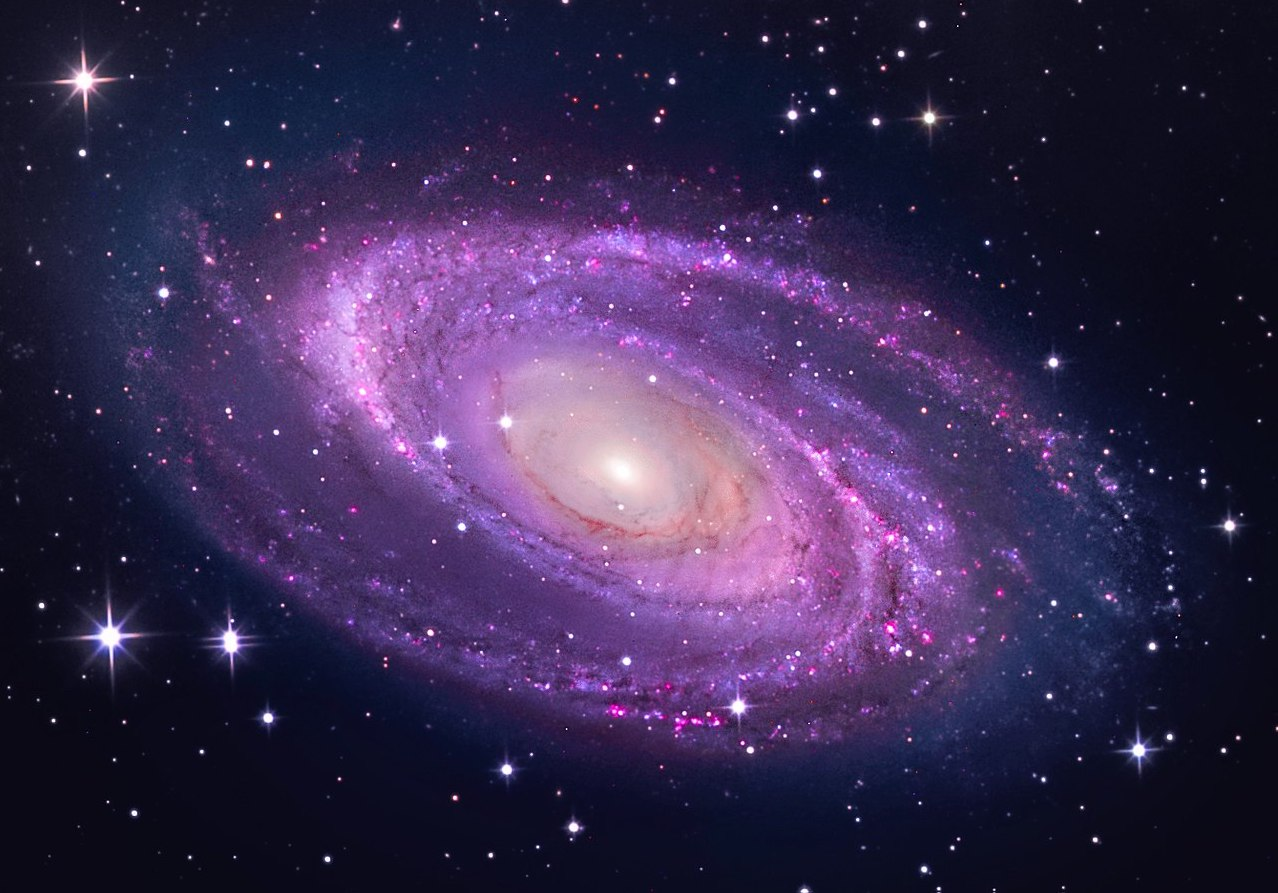
\includegraphics[width = 0.7\textwidth]{figures/M81.jpeg}
    \caption{Long exposure image of Messier 81 taken through a 20 inch telescope by astrophotographer \citet{adler2015}, taken with LRGB filters and a Hydrogen-$\alpha$ filter that was assigned to red. Overall 20 hours of exposures were taken.}
    \label{fig:M81}
\end{figure}

Perhaps the most well known examples of spiral structures in astrophysics are the grand design spirals of galaxies like Messier 81 (M81), shown in Figure~\ref{fig:M81}.
The disk of a galaxy rotates differentially, similarly to a circumstellar disk, resulting in an initially puzzling state of affairs.
If the material making up the spiral structure remains in the arm, then the pattern should be quickly destroyed since material in the inner disk orbits at a much greater rate than that in the outer disk.
This is known at the \textit{winding problem}, and it proved to be a serious challenge for early attempts to explain spiral structure in galaxies \citep{wilczynski1896,oort1962}.

The first major advance in our understanding of the origins of galactic spiral structure was made by Bertil Lindblad in the early 1960s. 
Lindblad proposed that spiral structure may be a quasi-stationary wave resulting from the superposition of multiple spiral modes.
In Lindblad's model, these modes were excited through the interaction of orbital motions and gravitational forces of the stars in the disk \citep{lindblad1963}.
This was a radical view at the time, as it was widely believed that spiral structure was induced by galactic-scale magnetic fields \citep[e.g.][]{hoyle1961,oki1964}.
The paradigm-shift would come shortly after with the seminal work by \citet{lin1964}, pioneering the \textit{density wave theory} picture of spiral structure.
In their view, spiral arms are quasi-static overdense regions of the disk resulting from periodic compression and rarefaction of disk material, similar to a traffic jam.
This, in combination with Lindblad's findings make up the \textit{Lin-Shu Hypothesis}, which states that galactic spiral structure is a stationary density wave, and that the spiral pattern is unchanged over long timescales apart from the overall rotation of the galaxy.
A more precise statement of the hypothesis is that the spiral is a marginally stable wave mode of the disk.

The Lin-Shu hypothesis is however not correct \citep{toomre1969,dobbs2014}
The spiral structure found in galaxies is indeed a density wave, but the wave is not a stationary, stable mode of the disk.
Instead the spiral arms are the result of the disk responding to a variety of gravitational disturbances such as nearby galaxies \citep{goldreich1965,julian1966}.
Indeed, the grand design spirals in M81 are thought to be the result of tidal-interactions with its companion galaxy Messier 82 \citep{yun1999a}.

Spiral arms similar to those found in galaxies have been observed in the disks around the stars HD~142529 \citep{christiaens2014}, MWC~758 \citep{benisty2015}, Elias~27 \citep{perez2016,huang2018}, IM~Lupi \citep{avenhaus2018,huang2018}, WaOph~6 \citep{huang2018}, HD~163296 \citep{calcino2022}, TW~Hya \citep{teague2022} and others \citep[and references therin]{dong2018}.
Figure~\ref{fig:mwc758} shows the double-armed spiral of MWC~758 in scattered light.
The origin of most of these spirals is still unknown \citep[e.g.][]{zhang2018}.
Of particular interest to us here are kinematic detections of planets located inside dust gaps \citep{pinte2018a,pinte2019,pinte2020,teague2021,teague2022}, since they are very well explained by the planet wake scenario, as we will see.

\begin{figure}
    \centering
    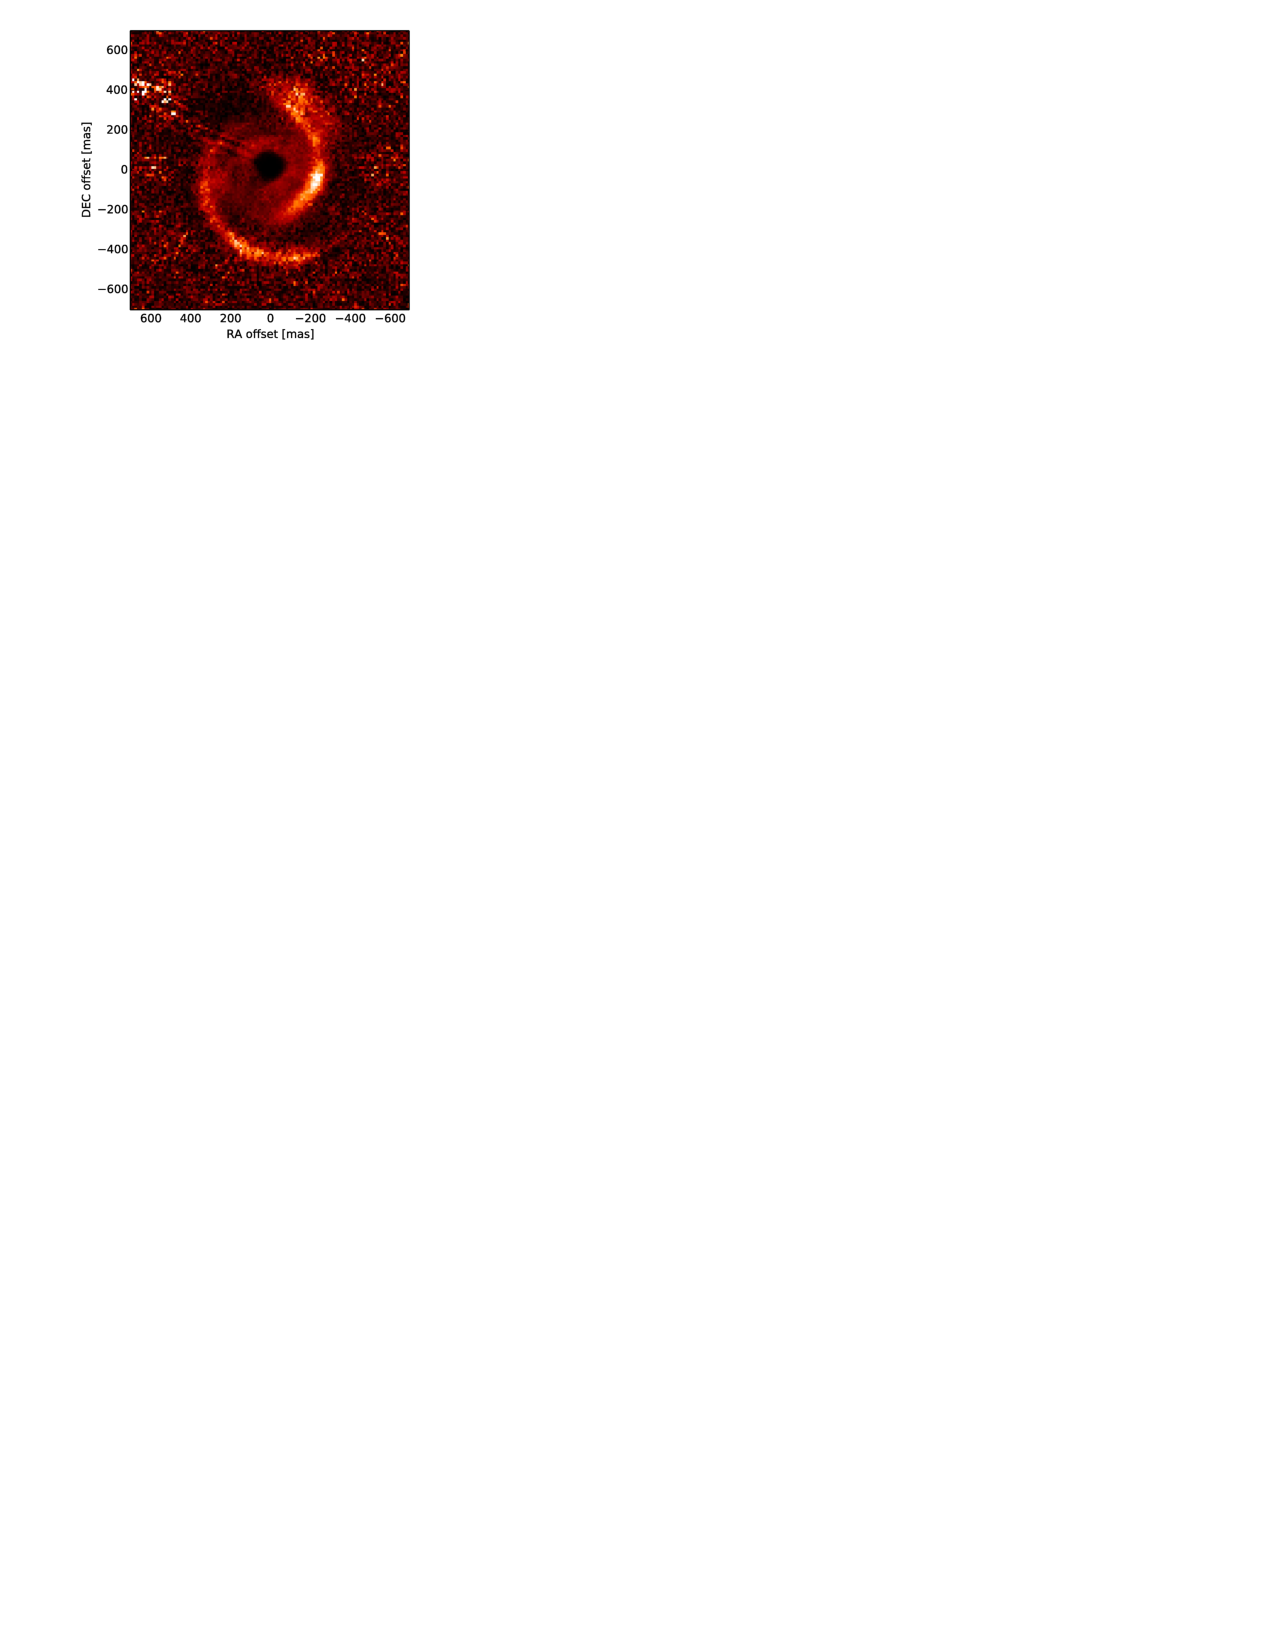
\includegraphics[width = 0.7\textwidth]{figures/mwc758.pdf}
    \caption{Polarised intensity image of the disk MWC~758 obtained in December 2014 with SPHERE \citep[e.g.][]{beuzit2019}. The colour scale is arbitrary. Two large spiral arms are clearly present in the disk \citep{benisty2015}. The origin of these spiral arms is still unknown.}
    \label{fig:mwc758}
\end{figure}

\subsection{Spiral structure preliminaries}
We now introduce the following concepts:
\begin{enumerate}
    \item The \textit{pitch angle} $\alpha$: of a spiral arm is defined as the angle between the tangent to the spiral at some radius $r$ and the circle with the same radius. 
    Thus $\alpha$ is in general a function of radius and $0 < \alpha < \pi/2$ by definition.
    \item $m$-fold \textit{rotational symmetry}: if a rotation of $2\pi/m$ radians results in no change to the disk surface density, that is $\Sigma(r,\phi)=\Sigma(r,\phi+\frac{2\pi}{m})$, then the disk is said to contain $m$ spiral arms and exhibits an $m$-fold rotational symmetry. 
    For example, a disk containing two spiral arms will be unchanged under a rotation of $180^\circ$ and so has $2$-fold rotational symmetry.
    \item \textit{Leading} and \textit{trailing} spiral arms: the tip of a leading spiral arm points in the direction of the bulk rotation of the disk, while the tip of a trailing arm points in the opposite direction to the rotation. 
    While it seems that leading arms may indeed be physically realised in the universe \citep[e.g.][]{vaisanen2008}, they are at minimum very rare. 
    We will be concerned only with trailing spirals in this thesis.
%    \item The \textit{pattern speed} $\Omega_\mathrm{p}$: In the Lin-Shu hypothesis the spiral structure is a fixed pattern that rotates rigidly. 
%    The angular speed of rotation of these spirals according to some inertial observer is known as the pattern speed $\Omega_\mathrm{p}$. 
%    More generally, the pattern speed is well defined so long as the spirals constitute a steady state solution in some rigidly rotating frame. 
%    As we will see, this is the case for the spiral wake generated by a perturbing planet on a circular orbit, in which case the pattern speed is simply equal to the orbital rotation of the planet
\end{enumerate}

Consider a disk containing a set of $m$ spiral arms such that is has $m$-fold symmetry. We may parameterise the curves defined by the centre of each of the spiral arms as
\begin{align}
    m\phi + f(r,t) = C \,\, \mathrm{mod} \,\, 2\pi, \label{eq:spiral_para}
\end{align}
where $C$ is a constant real number and $f$ is known as the \textit{shape function}. The \textit{radial wavenumber} $k$ is defined in terms of $f$ and is given by
\begin{align}
    k(r,t) \equiv \partial_r f(r,t).
\end{align}
For a counter-clockwise rotating disk we have $m>0$ and so $k>0$ corresponds to trailing arms while $k<0$ gives leading arms. 
The opposite is true for clockwise rotating disks with $m<0$. 
We will always assume both $k$ and $m$ are positive, corresponding to tailing arms in a counter-clockwise rotating disk. 
The pitch angle $\alpha$ of a spiral arm is given by
\begin{align}
    \mathrm{cot}\,\alpha = \left| r \partial_r \phi \right|,
\end{align}
where $r \partial_r \phi$ is evaluated along the curve that defines the spiral. In terms of the parameterisation \eqref{eq:spiral_para} we have $\partial_r[m\phi+f(r,t)] = m \partial_r \phi + k = 0$ giving
\begin{align}
    \alpha = \arctan \left( \frac{m}{kr} \right). \label{eq:pitchangle}
\end{align}

\subsection{No leading spirals}

In the previous section we stated that while leading spirals may exist in nature, they are at least much rarer that than trailing spirals; there are \textbf{no} known examples of leading spirals in circumstellar disks.
This is at least initially surprising. 
If the trailing spiral arms seen in astrophysical disks are steady-state solutions governed by Newtonian physics, which is fully time-reversible, surely the corresponding leading spirals solution is entirely equivalent?
\citet{lynden-bell1967} followed this argument to prove the \textit{anti-spiral} theorem, which states that if trailing spirals constitute a steady-state solution to time-reversible equations, then there necessarily exists an equivalent leading spiral solution.
Thus the apparent ubiquity of trailing spirals in nature tells us that either the governing physics is not time-reversible, or the spirals are not true steady-state solutions.
In the latter case spiral structure may be the result of a recent disturbance, or may be continuously regenerated for example by period tidal forcing.
This mimics the failing of the Lin-Shu hypothesis for galaxies, where spiral structure turned out to be the response of the disk to disturbances.
In Section~\ref{sec:planet_forcing} we will see that the perturbations driven periodically by a gravitating body embedded in a circumstellar disk result in a trailing spiral structure.

\section{The Linear Disk Response}

Before determining how the periodic forcing of the planet potential perturbs the disk, we must first determine how the disk responds to some small, generic disturbance.
The 2D inviscid equations of momentum and continuity expressed in terms of surface density are given by \citep{landau1959}
\begin{align}
    &\partial_t u + u \partial_r u + \frac{v}{r} \partial_\phi u - \frac{v^2}{r} = - \partial_r \Phi - \frac{1}{\Sigma} \partial_r P, \label{eq:mom_eq_u} \\ 
    &\partial_t v + u \partial_r v + \frac{v}{r} \partial_\phi v - \frac{uv}{r} = - \frac{1}{r} \partial_\phi \Phi - \frac{1}{r\Sigma} \partial_\phi P, \label{eq:mom_eq_v} \\
    &\partial_t \Sigma + \frac{1}{r} \partial_r (r \Sigma u) + \frac{1}{r} \partial_\phi (\Sigma v) = 0. 
    \label{eq:cont_2d}
\end{align}
Assuming a polytropic equation of state
\begin{align}
    P = K \Sigma^\gamma,
\end{align}
where $K$ is a constant and $\gamma$ is the adiabatic index. We then find the sound speed $c$ to be
\begin{align}
    c^2 = \partial_\Sigma P = \gamma K \Sigma^{\gamma-1}. \label{eq:cs_poly}
\end{align}
To simplify the equations we introduce the specific enthalpy $h$. Since the equation of state we are using is isentropic, we have $dh = dP / \Sigma$ giving
\begin{align}
    h = \int \frac{1}{\Sigma} dP = \int \frac{c^2}{\Sigma} d\Sigma = \frac{\gamma}{\gamma-1} K \Sigma^{\gamma-1}. \label{eq:enthalpy}
\end{align}
Note that
\begin{align}
    \partial_x h = \frac{\gamma}{\gamma - 1} K \partial_\Sigma (\Sigma^{\gamma-1}) \partial_x \Sigma = \gamma K \Sigma^{\gamma-2} \partial_x \Sigma,
\end{align}
such that the right-hand sides of Equations \eqref{eq:mom_eq_u} and \eqref{eq:mom_eq_v} become
\begin{align}
    - \partial_r \Phi - \frac{1}{\Sigma} \partial_r P = - \partial_r \Phi - \gamma K \Sigma^{\gamma-2} \partial_r \Sigma = - \partial_r (\Phi + h) \label{eq:mom_u_RHS},
\end{align}
and
\begin{align}
    - \frac{1}{r} \partial_\phi \Phi - \frac{1}{r\Sigma} \partial_\phi P = - \frac{1}{r} \partial_\phi (\Phi + h) \label{eq:mom_v_RHS},
\end{align}
respectively.

We now perform a linear perturbation study; we assume that the spiral waves in the disk constitute only a small perturbation from some background steady-state, and that the background state is axisymmetric.
We rewrite the quantities $\Sigma,\Phi,h,u,v$ as a combination of the background value (denoted by subscript 0) and a small perturbation  (denoted by $\delta$)
\begin{align}
    \Sigma &= \Sigma_0 + \delta\Sigma, \label{eq:pertsig} \\
    \Phi &= \Phi_0 + \delta\Phi, \label{eq:pertphi} \\
    h &= h_0 + \delta h, \label{eq:perth} \\
    v &= v_0 + \delta v, \label{eq:pertv} \\ 
    u &= \delta u, \label{eq:pertu}
\end{align}
where we note that $u_0=0$ since we assume no radial motion in the background state.
From Equations \eqref{eq:mom_eq_u} and \eqref{eq:mom_u_RHS}, and making use of the axisymmetry of the background state, we find the equation of motion for the background
\begin{align}
    \frac{v_0^2}{r} = \partial_r \left( \Phi_0 + h_0  \right), \label{eq:pertback}
\end{align}
which is the 2D equivalent of Equation~\eqref{eq:rotation}. 
Substituting \eqref{eq:pertsig}-\eqref{eq:pertu} into Equations \eqref{eq:mom_eq_u}, \eqref{eq:mom_eq_v}, \eqref{eq:mom_u_RHS}, \eqref{eq:mom_v_RHS}, discarding second order terms, and subtracting Equation~\eqref{eq:pertback} yields the linearised equations of motion 
\begin{align}
    \partial_t \delta u + \Omega \partial_\phi \delta u - 2 \Omega \delta v &= - \partial_r \left( \delta \Phi + \delta h  \right), \label{eq:mom_u_lin} \\
    \partial_t \delta v + \Omega \partial_\phi \delta v - 2 B \delta u &= - \frac{1}{r} \partial_\phi \left( \delta \Phi + \delta h  \right), \label{eq:mom_v_lin}
\end{align}
where we have also substituted $v_0=\Omega r$ and the second Oort constant $B = -r \partial_r \Omega / 2 -\Omega$, which is related to the epicyclic frequency as $\kappa^2 = -4 B \Omega$. 
The linearised equation of continuity is obtained similarly from \eqref{eq:cont_2d}
\begin{align}
    \partial_t \delta \Sigma + \frac{1}{r} \partial_r \left( r \Sigma_0 \delta u  \right) + \frac{\Sigma_0}{r} \partial_\phi \delta v + \Omega \partial_\phi \delta \Sigma. \label{eq:cont_lin}
\end{align}
We assume that the equations of motion \eqref{eq:mom_u_lin} and \eqref{eq:mom_v_lin} are solved by a summation of plane waves, where each perturbed quantity $a \in \left\{ \Sigma, \Phi, h, v, u \right\}$ can be written as
\begin{align}
    \delta a = \sum_m \delta a_m = \sum_m a_m(r) \exp \left[ i (m\phi - \omega t) \right]; \quad m \in \mathbb{Z}^{0+}, \label{eq:pert_sum_form}
\end{align}
where each $m$ component of the perturbation has $m$-fold symmetry and $a_m(r)$ is in general a complex function.
The physical perturbation is obtained by taking the real component $\mathrm{Re}(\delta a)$.
Substituting the summands of \eqref{eq:pert_sum_form} in place of the perturbations in our linearised equations yields
\begin{align}
    u_m (r) &= \frac{i}{\Delta_m} \left[ (\omega - m \Omega) \partial_r (\Phi_m + h_m) - \frac{2 m \Omega}{r} (\Phi_m + h_m) \right] \label{eq:lin_u_m}, \\
    v_m (r) &= - \frac{1}{\Delta_m} \left[ 2B \partial_r (\Phi_m + h_m) + \frac{m(\omega - m \Omega)}{r} (\Phi_m + h_m) \right] \label{eq:lin_v_m}, \\
    \Sigma_m (r) &= \frac{1}{r(\omega - m \Omega)} \left[ m \Sigma_0 v_m -i \partial_r (r u_m \Sigma_0) \right] \label{eq:lin_cont_m},
\end{align}
where
\begin{align}
    \Delta_m \equiv \kappa^2 - (\omega - m \Omega)^2. \label{eq:def_delta_m}
\end{align}
Finally, we must linearise the equation of state.
Taking Equation~\eqref{eq:enthalpy} and expanding in $\delta \Sigma / \Sigma_0$
\begin{align}
    h_0 + \delta h = \frac{\gamma}{\gamma - 1} K \Sigma_0^{\gamma - 1}(1 + \frac{\delta\Sigma}{\Sigma_0})^{\gamma-1} = \frac{\gamma}{\gamma - 1} K \Sigma_0^{\gamma - 1} + \gamma K \Sigma_0^{\gamma-1} \frac{\delta\Sigma}{\Sigma_0} + \mathcal{O}(\left(\delta\Sigma / \Sigma_0\right)^2).
\end{align}
Now substituting Equations \eqref{eq:cs_poly} and \eqref{eq:enthalpy}, and taking only one component of the perturbation, we find
\begin{align}
    h_m \simeq c_0^2 \frac{\Sigma_m}{\Sigma_0}, \label{eq:lin_EOS_m}
\end{align}
where $c_0$ is the unperturbed sound speed.

With Equations \eqref{eq:lin_u_m}, \eqref{eq:lin_v_m}, \eqref{eq:lin_cont_m} and \eqref{eq:lin_EOS_m} we have four constraints on the five state variables $\Sigma_m, \Phi_m, h_m, v_m$ and $u_m$.
We therefore now have a system of equations describing the \textit{linear response} of the disk $\Sigma_m$ for the azimuthal wave mode $m$, to the potential component $\Phi_m$.
By summing over all modes, we can calculate the \textit{global} response of the disk to some imposed gravitational potential.
This however, cannot be done analytically.

\subsection{Tightly-wound density waves}

We now apply \textit{WKB approximation}, which will allow to find \textit{local} analytic solutions.
For spiral density waves this is equivalent to assuming that the spirals are \textit{tightly-wound} and thus is also called the \textit{tight-winding approximation}.
For a spiral with shape function $f$ let $\lambda_r$ be the radial separation between adjacent arms for fixed $\phi$, such that
\begin{align}
    2\pi = \left| f(r+\lambda_r, t) - f(r,t) \right|.
\end{align}
If we assume that the spirals are indeed tightly-wound such that $\alpha\rightarrow 0$, then we have that $f(r+\lambda_r,t)=f(r,t) + \lambda_r \partial_r f |_{r,t}$. 
Recalling that $\partial_r f |_{r,t}$ is none other than the radial wavenumber $k$, we find
\begin{align}
    2 \pi &= \left| f(r,t) + \lambda_r \partial_r f |_{r,t} - f(r,t) \right|, \\
    &= \lambda_r | k |, \\
    \Rightarrow \lambda_r &= \frac{2 \pi}{|k|},
\end{align}
and so we find that the radial wavenumber $r$ has the usual relationship with the radial wavelength $\lambda_r$. 
Substituting Equation~\eqref{eq:pitchangle} gives
\begin{align}
    \frac{\lambda_r}{r} = \frac{2 \pi}{|rk|} =  \frac{2 \pi \tan \alpha}{m},
\end{align}
and so an equivalent condition for the tight-winding approximation is that $|rk| \gg 2 \pi$. 
This equivalency however does not hold for very large $m$ since the right-hand side above can then approach zero regardless of $\alpha$, and is also invalid for $m = 0$ ie. purely radial perturbations.

\subsection{Perturbed potential under WKB}

We can write the perturbed spiral surface density for some mode $m$ in a form similar to \eqref{eq:pert_sum_form} where we instead separate the rapid variations in density moving from one arm to another, and the slower variation while moving along a particular arm
\begin{align}
    \delta \Sigma_m = \Sigma_m \exp \left[ i \left( m \phi + f(r,t)  \right)  \right]. \label{eq:sigma_WKB}
\end{align}
To determine the disk response we must find the gravitational potential due to this perturbed surface density, which is done by solving Poisson's equation
\begin{align}
    \nabla^2 \delta \Phi_m = 4 \pi G \delta \Sigma_m \delta(z), \label{eq:poisson_pert}
\end{align}
where $\delta(z)$ is the Dirac delta since we assume the disk is infinitely thin. 
The solution under the WKB approximation is \citep[e.g.][]{binney2008}
\begin{align}
    \delta \Phi_m &= - \frac{2 \pi G}{|k|} \Sigma_m \exp \left[ i \left( m \phi + f(r,t)  \right)  \right], \\
    \Rightarrow \Phi_m &= - \frac{2 \pi G}{|k|} \Sigma_m. \label{eq:phi_m_sigma_m}
\end{align}

\subsection{The Lin-Shu dispersion relation} \label{sec:linshu}

We now rewrite each coefficient $a_m(r)$ for each term $\delta a_m$ of some perturbed quantity $\delta a$ as
\begin{align}
    a_m(r) = A_m(r) \exp \left[ i f(r) \right] = A_m(r) \exp \left[ i \int^r k(r') \, dr' \right], \label{eq:WKB_form}
\end{align}
where, similarly to \eqref{eq:sigma_WKB}, $F(r)$ is a slowly varying function of radius and the exponential encapsulates more rapid variations. 
The radial derivative of $a_m$ is then
\begin{align}
    \partial_r a_m(r) = \left( \partial_r A_m + ikA_m  \right) \exp \left[ i \int^r k(r') \, dr' \right].
\end{align}
Under the WKB approximation we have $|kr|\gg 2 \pi$.
Since $A_m(r)$ is a smoothly varying function of r, $|\partial_r A_m| \sim \mathcal{O}(A_m / r)$, yielding $\partial_r A_m \ll |k A_m|$.
We therefore neglect the first term above, giving
\begin{align}
    \partial_r a_m(r) = ikA_m \exp \left[ i \int^r k(r') \, dr' \right] + \mathcal{O}\left(\frac{1}{|kr|}\right) \approx ik a_m(r). \label{eq:app_radial_deriv}
\end{align}
Thus assuming the form \eqref{eq:WKB_form} for the quantities in Equations \eqref{eq:lin_u_m} - \eqref{eq:lin_cont_m} and applying the WKB approximation yields
\begin{align}
    u_m(r) &= - \frac{k(\omega-m\Omega)}{\Delta_m} (\Phi_m + h_m), \label{eq:u_m_disp} \\
    v_m(r) &= - \frac{2ikB}{\Delta_m} (\Phi_m + h_m), \label{eq:v_m_disp} \\
    \Sigma_m(r) &= \frac{k \Sigma_0}{\omega-m\Omega} u_m, \label{eq:sigma_m_disp}
\end{align}
where the error is for all cases $\mathcal{O}(1/|kr|)$, as we have approximated the radial derivatives by \eqref{eq:app_radial_deriv} and dropped terms proportional to $1/r$ in favour of terms proportional to $k$.
Finally, we may combine Equations \eqref{eq:lin_EOS_m}, \eqref{eq:phi_m_sigma_m}, \eqref{eq:u_m_disp} and \eqref{eq:sigma_m_disp} to find the dispersion relation for tightly-wound density waves in a rotating gas disk
\begin{align}
    \left( \omega - m \Omega  \right)^2 &= \kappa^2 - 2 \pi G |k| \Sigma_0 + c_0^2 k^2. \label{eq:lin_shu_disp}
\end{align}
This result is known as the \textit{Lin-Shu Dispersion Relation} \citep{lin1964}.

\subsection{Stability}

If the right-hand side of the Lin-Shu dispersion relation \eqref{eq:lin_shu_disp} is negative, that is $(\omega - m \Omega)^2 < 0$, then $\omega$ will become imaginary resulting in the exponential growth of the density perturbation $\delta \Sigma$.
By requiring that $(\omega - m \Omega)^2 > 0$ for all possible $k$, the disk stability criterion $Q$ is derived \citep{toomre1964}
\begin{align}
    Q(r) \equiv \frac{c_0 \kappa}{\pi G \Sigma} > 1.
\end{align}
Disk regions where $Q(r) < 1$ are subject to local unstable growth for certain values of $k$.
This can result in the fragmentation of the disk, and may be a pathway to the formation of giant planets \citep{boss1997}.
%Planet formation through this mechanism is known as the Gravitational Instability model \fct, and it is similar in spirit to star formation through the Jeans instability \citep{jeans1902}.

\section{Planet Forcing} \label{sec:planet_forcing}

Armed with the Lin-Shu dispersion relation that encodes the linear disk response to a disturbance in terms of density wave theory, we are ready to investigate the effects of the gravitational perturbation induced by an embedded planet.
This will in turn allow us to study the generation and propagation of the resultant spiral structure.

\subsection{Lindblad resonances}

Let $(r,\phi)$ be polar coordinates centred on some star with mass $M_\star$.
We place a planet of mass $M_{\rm p} \ll M_\star$ on a circular orbit of radius $r_{\rm p}$ around the star.
The angular velocity of the planet $\Omega_{\rm p}$ will be given by 
\begin{align}
    \Omega_{\rm p}^2 = \Omega_{\rm K}(r_{\rm p}) = \frac{G M_\star}{r_{\rm p}^3} = \frac{1}{r_{\rm p}} \left( \frac{d\Phi_\star}{dr} \right) _{r_{\rm p}},
\end{align}
where $\Phi_\star$ is the gravitational potential for a point mass
\begin{align}
    \Phi_\star = - \frac{G m_\star}{r}.
\end{align}
Similarly, the angular velocity of some other test particle on a circular orbit (neglecting the influence of the planet) will be
\begin{align}
    \Omega_0^2 = \frac{1}{r} \frac{d\Phi_\star}{dr}.
\end{align}
Now consider the problem in a rotating frame such that the planet is always at $\phi=0$, which will remove the time dependence from the planet potential. 
The corresponding transformation will be given by $\phi \rightarrow \phi - \Omega_{\rm p} t$.
The Lagrangian for a test particle in such a frame is
\begin{align}
    \mathcal{L} = \frac{1}{2} \left[ \dot{r}^2 + r^2 \left( \dot{\phi} + \Omega_{\rm p}  \right)^2 \right] - \Phi (r, \phi),
\end{align}
where $\Phi (r,\phi) = \Phi_\star (r) + \Phi_{\rm p} (r, \phi)$ is the total potential from both the star and planet.
From the Euler-Lagrange equations we find the equations of motion to be
\begin{align}
    \ddot{r} &= r \left( \dot{\phi} + \Omega_{\rm p} \right)^2 - \partial_r \Phi, \label{eq:EOM_rad} \\
    r^2 \ddot{\phi} &= - 2 r \dot{r} \left( \dot{\phi} + \Omega_{\rm p}  \right) - \partial_\phi \Phi. \label{eq:EOM_az}
\end{align}
We now perform a perturbation study using the change of variables $r(t) \rightarrow r + \delta r (t)$  and $\phi (t) \rightarrow \phi (t) + \delta \phi (t)$ where we assume that $\delta r \ll r$ and $\delta \phi \ll \phi$.
We will similarly assume that $\Phi_{\rm p} \ll \Phi_\star$.
Thus the derivatives transform to first order as
\begin{align}
    \partial_r &\rightarrow \partial_r + \delta r \partial_r^2 r, \\
    \partial_\phi &\rightarrow \partial_\phi + \delta \phi \partial_r^2 \phi.
\end{align}
The zeroth order terms of \eqref{eq:EOM_rad} and \eqref{eq:EOM_az} give 
\begin{align}
    r \left( \dot{\phi} + \Omega_{\rm p}  \right)^2 &= \frac{d\Phi_\star}{dr} , \\
    \ddot{\phi} &= 0,
\end{align}
which are just the usual equations for centripetal acceleration. 
They are solved simply by associating $\dot{\phi}$ appropriately with $\Omega$ by considering the transformation to the rotating frame, yielding
\begin{align}
    \dot {\phi} &= \Omega - \Omega_{\rm p}, \\
    \Rightarrow \phi &= \left( \Omega - \Omega_{\rm p} \right) t,
\end{align}
where the constant of integration is set to zero without loss of generality.
We are now free to consider in isolation the first order terms of \eqref{eq:EOM_rad} and \eqref{eq:EOM_az}, which reduce to 
\begin{align}
    \ddot{\delta r} + \left( \frac{d^2\Phi_\star}{dr^2} - \Omega^2 \right) \delta r &= 2 r \Omega \dot{\delta \phi} - \partial_r \Phi_{\rm p}, \label{eq:lin_rad_lindblad} \\
    \ddot{\phi} + \frac{2 \Omega}{r} \dot{\delta r} &= - \frac{1}{r^2} \partial_\phi \Phi_{\rm p}. \label{eq:lin_az_lindblad}
\end{align}
We will now specify a form for the planet potential $\Phi_{\rm p}$.
Starting with the usual point mass potential centred on the planet we have
\begin{align}
    \Phi_{\rm p} (r,\phi) &= -\frac{G M_{\rm p}}{|\bf{r} - \bf{r_{\rm p}}|}, \\
    &= -\frac{G M_{\rm p}}{\sqrt{(r_{\rm p} - r \cos \phi)^2 + (r \sin \phi)^2}}, \\
    &= -\frac{G M_{\rm p}}{\sqrt{r^2 - 2 r r_{\rm p} \cos \phi + r_{\rm p}^2}}, \\
    &= -\frac{G M_{\rm p}}{r_{\rm p}} \left[ \mathcal{R}^2 - 2 \mathcal{R} \cos \phi + 1\right]^{-\frac{1}{2}},
\end{align}
where $\mathcal{R} = r / r_{\rm p}$.
To investigate the influence of this potential perturbing our test particles we will decompose it using a Fourier series.
The potential must by invariant under $\phi \rightarrow -\phi$ as well as $2 \pi$ periodic in $\phi$, motivating the form\footnote{The origin of our chosen coordinates is the centre of the star, but this point will not be the barycentre of the system. Our frame is therefore non-inertial and results in an additional acceleration which is typically included as the gradient of an additional potential contribution, the so-called indirect potential \citep{goldreich1980}. However the contribution is small and so is neglected even in detailed calculations of the linear disk response to tidal forcing by a planet \citep[see for example][]{bae2018a,miranda2019a}.}
\begin{align}
    \Phi_{\rm p}(r,\phi) = \sum_{m=0}^\infty \Phi_m (r,\phi) = \sum_{m=0}^\infty V_m (r) \cos (m \phi), \label{eq:fourier_planet}
\end{align}
where in our case the Fourier coefficients are given by 
\begin{align}
    V_m (r) &= - \frac{2}{\pi} \frac{G M_{\rm p}}{r_{\rm p}} \int_0^\pi  \left( \mathcal{R}^2 - 2 \mathcal{R} \cos \phi + 1\right)^{-\frac{1}{2}} \cos (m \phi) \, d\phi, \\
    &= \frac{\delta_{m0} - 2}{2} \frac{G M_{\rm p}}{r_{\rm p}} \, b_{1/2}^m (\mathcal{R}),
\end{align}
where $b_{1/2}^m (\mathcal{R})$ are the Laplace coefficients defined in \citet{brouwer1961}.
Figure~\ref{fig:planet_fourier} shows the first $m$ Fourier components of the planet potential $\Phi_m$, where the star is located at the origin and the planet is at the point $(1,0)$.
Each of these components results in the periodic driving of perturbations in the disk, with a period equal to $2\pi / (m \Omega_{\rm p})$.

Here we are primarily concerned with the \textit{form} of the decomposition \eqref{eq:fourier_planet} which is actually quite general and can represent a variety of potentials including the bars often found in spiral galaxies.
Next we will substitute a single Fourier component in place of the planet potential to determine the response for \textit{each individual component}.
Note that we will also ignore the contribution of $\delta \phi$ to $\Phi_{\rm p}$, assuming that $\phi$ corresponds to the zeroth order solution where $\phi = (\Omega - \Omega_{\rm p}) t$. 

\begin{figure}
    \centering
    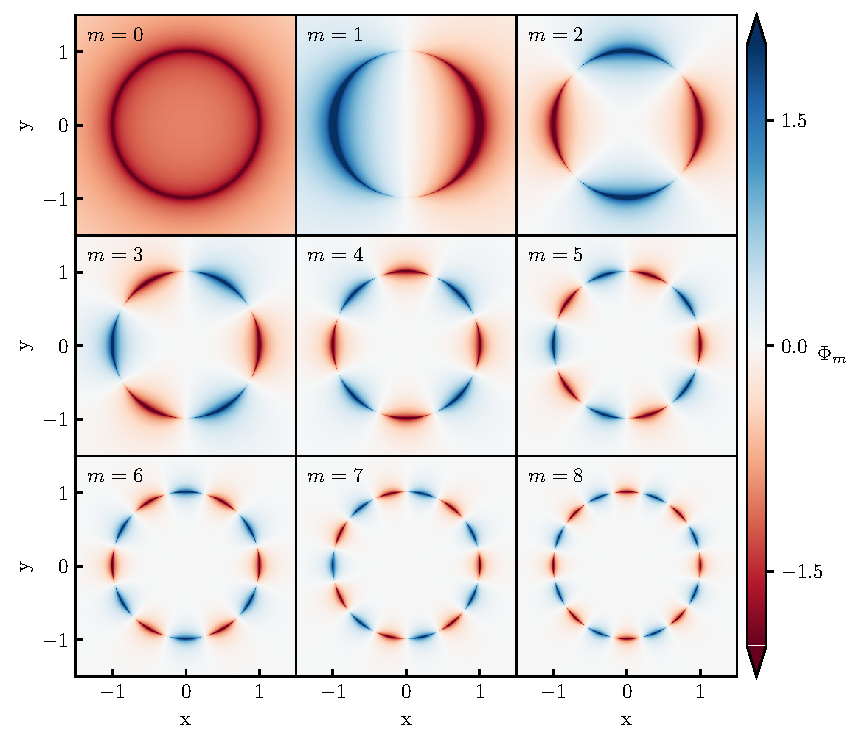
\includegraphics[width = 0.95\textwidth]{figures/planet_components.pdf}
    \caption{The first 9 Fourier components of the planet potential $\Phi_m(r,\phi) = V_m(r) \cos (m \phi)$, where the star is located at $(x,y) = (0,0)$ and the planet at $(1,0)$. The units are dimensionless such that $G=M_{\rm p}=1$. The Laplace coefficients $b_{1/2}^m$ were calculated using the \textsc{Python} package \textsc{PyLaplace} \citep{paardekooper2019a}}
    \label{fig:planet_fourier}
\end{figure}

From Equation~\eqref{eq:fourier_planet} we find the following derivatives
\begin{align}
    \partial_r \Phi_m (r, \phi) &= \frac{dV_m(r)}{dr} \cos (m \phi) \\
    \partial_\phi \Phi_m (r, \phi) &= - m V_m(r) \sin (m \phi),
\end{align}
and so Equation~\eqref{eq:lin_az_lindblad} becomes
\begin{align}
    \ddot{\phi} = - \frac{2 \Omega}{r} \dot{\delta r} + \frac{m V_m}{r^2} \sin \left( m [ \Omega - \Omega_{\rm p}] t\right),
\end{align}
and integrating gives
\begin{align}
    \dot{\phi} = - \frac{2 \Omega}{r} \delta r - \frac{V_m}{(\Omega - \Omega_{\rm p}) r^2} \cos \left( m [ \Omega - \Omega_{\rm p}] t \right).
\end{align}
Substituting this into \eqref{eq:lin_rad_lindblad} yields
\begin{align}
    \ddot{\delta r} + \kappa^2 \delta r = \Psi_m(r) \cos (m [ \Omega - \Omega_{\rm p}] t), \label{eq:lindblad_forcing}
\end{align}
where
\begin{align}
    \kappa^2 \equiv \frac{d^2 \Phi_\star}{dr^2} + 3 \Omega^2 = r \frac{d \Omega^2}{dr} + 4 \Omega^2,
\end{align}
is the usual epicyclic frequency already introduced. In addition, we define the forcing function $\Psi_m(r)$ as
\begin{align}
    \Psi_m(r) \equiv - \left( \frac{dV_m}{dr}+ \frac{2 \Omega}{(\Omega - \Omega_{\rm p})r} V_m \right).
\end{align}
Equation~\eqref{eq:lindblad_forcing} is a second order, inhomogeneous differential equation in the form of a driven harmonic oscillator.
The general solution $g(t)$ is given by 
\begin{align}
    g(t) = A_1 \mathcal{H}(t) + A_2 \mathcal{P}(t),
\end{align}
where $\mathcal{H}(t)$ is the solution to the homogeneous equation where the right-hand side is zero, $\mathcal{P}(t)$ is a particular solution to the inhomogeneous equation, and $A_1$ and $A_2$ are the amplitudes of each.
Physically, $A_1 \mathcal{H}(t)$ corresponds to the ``free'' solution in the absence of forcing by the planet potential, and a non-zero value of $A_1$ results in particle orbits that are not closed.
$A_2 \mathcal{P}(t)$ corresponds to the driven solution and is what we are interested in here.
We solve for the driven solution using the ansatz $\delta r (t) = A \cos (m [\Omega - \Omega_{\rm p}]t)$, with the result that the amplitude of the response to the planet forcing is given by 
\begin{align}
    A = \frac{\Psi_m (r)}{\Delta_m},
\end{align}
where $\Delta_m$ is as defined in Equation~\eqref{eq:def_delta_m}, and we have $\omega = m \Omega_{\rm p} $.
From this, we see that the forcing amplitude $A$ becomes very large as $\Delta_m \rightarrow 0$.
$\Delta_m = 0$ is therefore the condition for a \textit{Lindblad Resonance}; it determines the region where the response to periodic forcing by a particular component of the planet potential is greatest.
This is also the condition where the Lin-Shu dispersion relation breaks down as Equations \eqref{eq:lin_u_m} and \eqref{eq:lin_v_m} become singular.

From Equation~\eqref{eq:rotation}, we have that for material in a gas disk $\kappa = \Omega \approx \Omega_{\rm K}$.
Thus disk material is most effectively excited by the planet potential component $\Phi_m$ in the region where
\begin{align}
    \Omega_{\rm K}^2 = m^2 (\Omega_{\rm K} - \Omega_{\rm p})^2.
\end{align}
By substituting Equation~\eqref{eq:point_pot} we obtain the \textit{Lindblad radii}
\begin{align}
    r_{\rm L}^\pm(m) = \left( 1 \pm \frac{1}{m} \right)^\frac{2}{3} r_{\rm p}, \label{eq:lind_loc}
\end{align}
which are the positions of the $m$th Lindblad resonances, where $r_{\rm L}^-$ is interior to the planets orbit and $r_{\rm L}^+$ is exterior to the planets orbit.
The Lindblad resonances are spatially segregated but become densely packed near $r_{\rm p}$ as $m$ becomes large, as shown in Figure~\ref{fig:lindblad}.
This segregation allows us to consider each resonance location as driven by only the $m$th component of the planet potential.
This breaks down for large $m$ as the resonances are no longer clearly separated.

The pressure support of the disk results in a slight modification of $\Omega$ from $\Omega_{\rm K}$ as seen in Equation~\eqref{eq:rotation}.
This results in the radial shifting of the resonance positions \citep{artymowicz1993a}.
Resonance-shifting is important for calculating the total resultant torque on the disk, but affects the structure of excited waves only minimally and so we will ignore it here.

\begin{figure}
    \centering
    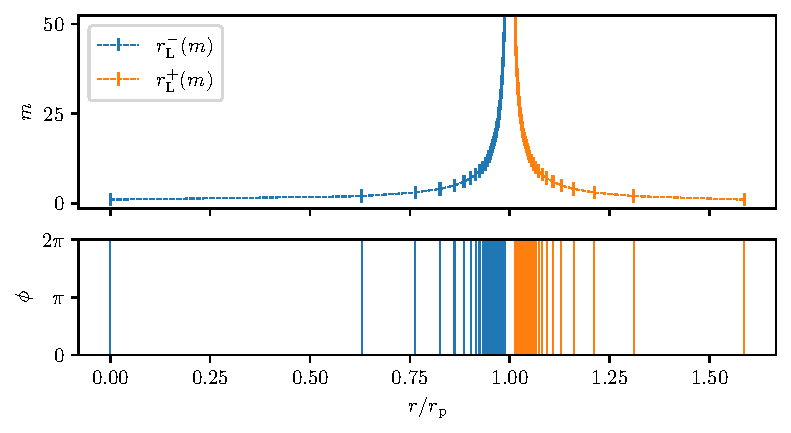
\includegraphics[width = 0.9\textwidth]{figures/lindblad_two_panel.pdf}
    \caption{Lindblad resonance positions as given by Equation~\eqref{eq:lind_loc}. The bottom panel shows the physical radial locations in the disk where these resonances occur for different $m$, with the inner resonances coloured blue and the outer resonances coloured orange. The top panel shows how these position are related to $m$, and demonstrates the asymptotic behaviour of the resonance position $r_{\rm L}^\pm \rightarrow r_{\rm p}$ as $m \rightarrow \infty$.}
    \label{fig:lindblad}
\end{figure}

\subsection{The planet wake} \label{sec:planetwake}

Following closely the work by \citet{ogilvie2002}, we will use phase arguments to determine the shape of the planet wake in the linear density wave theory paradigm.
However we will not follow exactly their original derivation.
We will instead obtain the more general form for the wake shape.
Similarly to in Section~\ref{sec:linshu}, we can write linear wave quantities in a 2D gas disk as 
\begin{align}
    \delta a_m = A_m(r) \exp{i \Theta_m},
\end{align}
where the amplitude $A_m(r)$ varies slowly with radius and the phase
\begin{align}
    \Theta_m = \int^r k(r') \, dr' + m (\phi - \Omega_p t),
\end{align}
varies rapidly with radius. 
Again only the real component is physically relevant, and we have written $\omega = m \Omega_p$ as we are assuming the waves are generated by an embedded planet.
To investigate the shape of the spiral wake we will look for lines of constant phase that are defined by the condition $\frac{d\Theta_m}{dr} = 0$ and so 
\begin{align}
    \frac{d\phi}{dr} = - \frac{k}{m}. \label{eq:spiral_km}
\end{align}
This is the same as the relation used to find the pitch angle of the spiral shape in Equation~\eqref{eq:pitchangle}.
Assuming Keplerian rotation such that $\kappa=\Omega=\Omega_{\rm K}$, we can find $k$ from the Lin-Shu Dispersion relation \eqref{eq:lin_shu_disp}
\begin{align}
    k^2 &= \frac{m^2 \left( \Omega - \Omega_{\rm p} \right)^2 - \kappa^2}{c^2}, \\
    &= \frac{m^2 \Omega_{\rm K}^2}{c^2} \frac{1}{r_{\rm p}^3} \left[ r^{3/2} - \left( r_{\rm L}^+ \right)^{3/2} \right] \left[ r^{3/2} - \left( r_{\rm L}^- \right)^{3/2} \right].
\end{align}
The tidal forcing of the planet results in density waves launched at the Lindblad resonances, with those launched at $r_{\rm L}^-$ and $r_{\rm L}^+$ propagating inwards and outwards through the disk respectively \citep{goldreich1978,goldreich1979}.
Figure~\ref{fig:wakes_m3} shows the shape of the $m=3$ spiral waves generated at the $r_{\rm L}^\pm (m=3)$ Lindblad resonances as they propagate away from the planet.
The shape of these spirals is calculated as follows.
\begin{figure}
    \centering
    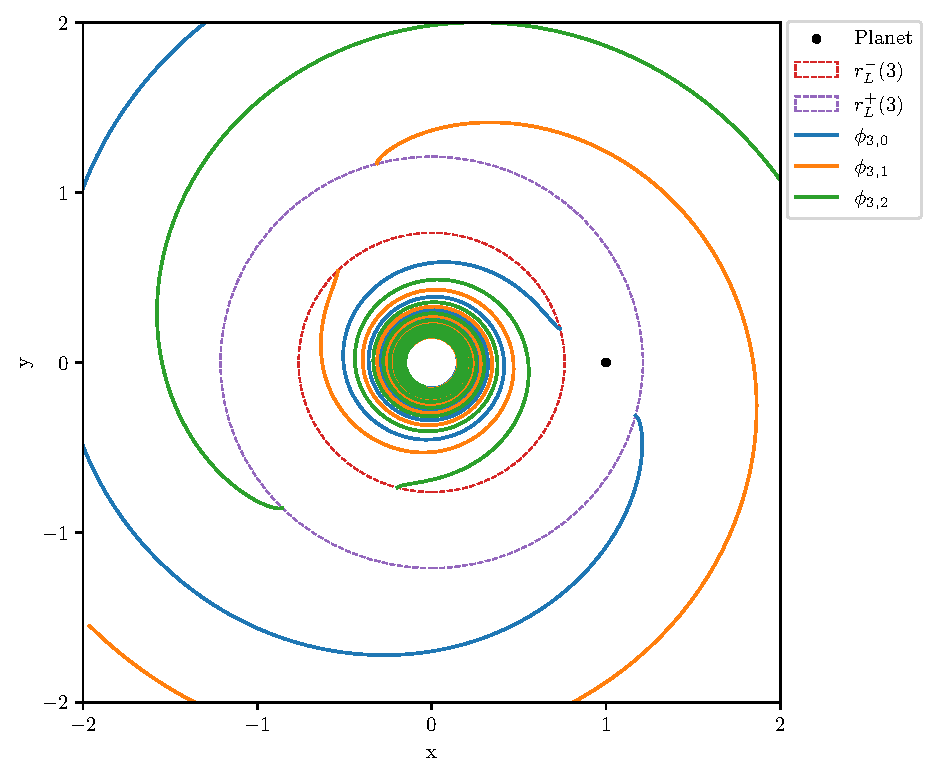
\includegraphics[width = 0.9\textwidth]{figures/wakes_m3.pdf}
    \caption{Schematic overview of the $m=3$ mode excited in a Keplerian disk. The disk has sound speed $c \propto r^{-1/4}$ where the aspect ratio at the planet is $(H/r)_{\rm p} = 0.1$.
    The planet is placed at $(1,0)$ and the inner and outer Lindblad resonances are shown by the red and purple dashed lines respectively.
    The blue, orange and green solid lines show lines of constant phase for the $n=0,1,2$ spiral arms excited at the resonances as they propagate inwards and outwards in the disk.
    These lines were calculated using Equations \eqref{eq:phase} -- \eqref{eq:planet_wake}.}
    \label{fig:wakes_m3}
\end{figure}
Placing ourselves in the frame where the planet is stationary at $\phi = 0$, we can find the phase of the spiral waves simply by integrating Equation~\eqref{eq:spiral_km} giving \citep{bae2018a}
\begin{align}
    \phi_m (r) = \phi_m(r_{\rm L}^\pm) - \int_{r_{\rm L}^\pm}^r \frac{k(r')}{m} \, dr', \label{eq:phase}
\end{align}
which consists of a constant offset $\phi_m(r_{\rm L}^\pm)$ term that gives the azimuthal launching location, plus a term that varies with radius.
For the waves launched at the Lindblad resonances, the constant offset term can be found from the asymptotic behaviour of the Airy function \citep{ward1986}. 
For the $n$th arm of the $mth$ mode, where $n = 0, 1, ..., m-1$ the offset is given by 
\begin{align}
    \phi_{m,n}(r_{\rm L}^\pm) = - \sign (r_{\rm L}^\pm - r_{\rm p}) \frac{\pi}{4m} + 2 \pi\frac{n}{m}. \label{eq:spiral_offset}
\end{align}
Now considering the $n=0$ arm, we see from the above that it launches closest to $\phi=0$ and thus closest to the planet.
For large $m$, we find that the constant offset term $\phi_{m,0}(r)$ becomes independent of $m$.
In addition, we have that $r_{\rm L}^\pm \rightarrow r_{\rm p}$ as $m \rightarrow \infty$.
This results in the formation of a coherent, one-armed spiral wave centred on the planet, as \eqref{eq:phase} and \eqref{eq:spiral_offset} reduces to
\begin{align}
    \phi_{\infty,0}(r) = - \int_{r_{\rm p}}^ r \frac{\Omega(r') - \Omega_{\rm p}}{c(r')} \, dr'. \label{eq:planet_wake}
\end{align}
Because the $n=0$ waves launch almost in phase nearby the planet, as seen in Figure~\ref{fig:planet_wake}, the planet wake is always centred on the planet location. 
The above result was first found by \citet{ogilvie2002}, although they wrote it in a different form. 
They dubbed the resultant spiral wave the planet ``wake'' in analogy with the Kelvin wedge produced by a ship moving through water.
The form shown above was first given in \citet{rafikov2002a}.

\begin{figure}
    \centering
    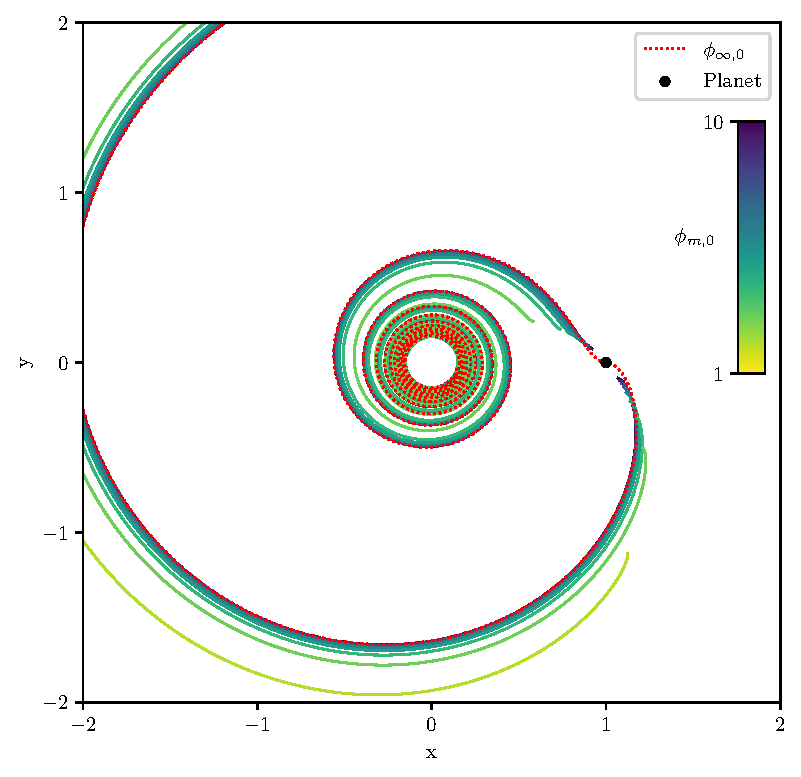
\includegraphics[width = 0.8\textwidth]{figures/planet_wake_shape.pdf}
    \caption{Plot of the $n=0$ spiral arms defined by the lines of constant phase $\phi_{m,0}$ for modes $m=1,...,10$ (solid lines).
    $\phi_{\infty,0}$ is shown with the red dotted line.
    The planet is placed at $(1,0)$ once again and the disk parameters are as in Figure~\ref{fig:wakes_m3}.
    We see that asymptotically $\phi_{m,0}$ approaches the planet wake shape $\phi_{\infty,0}$ as the line of constant phase loses its $m$ dependence for large $m$.}
    \label{fig:planet_wake}
\end{figure}

Ogilvie and Lubow also investigated the degree to which the constructive interference along $\phi_{\infty,0}$ fails.
To do this they calculated the relative error $\Delta_m$ in the phase for each $m$ caused by the approximation we have performed above.
Note that this is not the same quantity as we defined in \eqref{eq:def_delta_m}.
Figure~\ref{fig:delta_m} shows $\Delta_m$ in both the outer and inner disk, for multiple values of $m$.
We see that in general, the approximation improves for larger $m$.
Additionally, the behaviour in the inner and outer disk is very different.
Ogilvie and Lubow found that $\Delta_m \sim \mathrm{constant}$ as $r \rightarrow \infty$, while $\Delta_m$ diverges as $r \rightarrow$ 0, and that for any fixed $r$, $\Delta_m \rightarrow 0$ as $m \rightarrow \infty$.
Thus the accuracy of the one-armed wake shape \eqref{eq:planet_wake} is in general better in the outer disk than the inner disk, and also depends on the importance of each mode.
If the wave is dominated by large $m$ then \eqref{eq:planet_wake} holds everywhere except for very small disk radii, while always failing if dominated by $m=1$ or $2$ \citep{ogilvie2002}.
The dominating azimuthal mode for tidal forcing by a planet is $m_{\rm D} \approx 1/2 \left( H/r \right)_{\rm p}^{-1}$ \citep{goldreich1980}, and so for observed protoplanetary disks $m_{\rm D} \gtrsim 5$ \citep{law2021a}. 
The coherent planet wake picture should therefore hold well except for at small disk radii.

\begin{figure}
    \centering
    \begin{subfigure}[b]{0.49\textwidth}
        \centering
        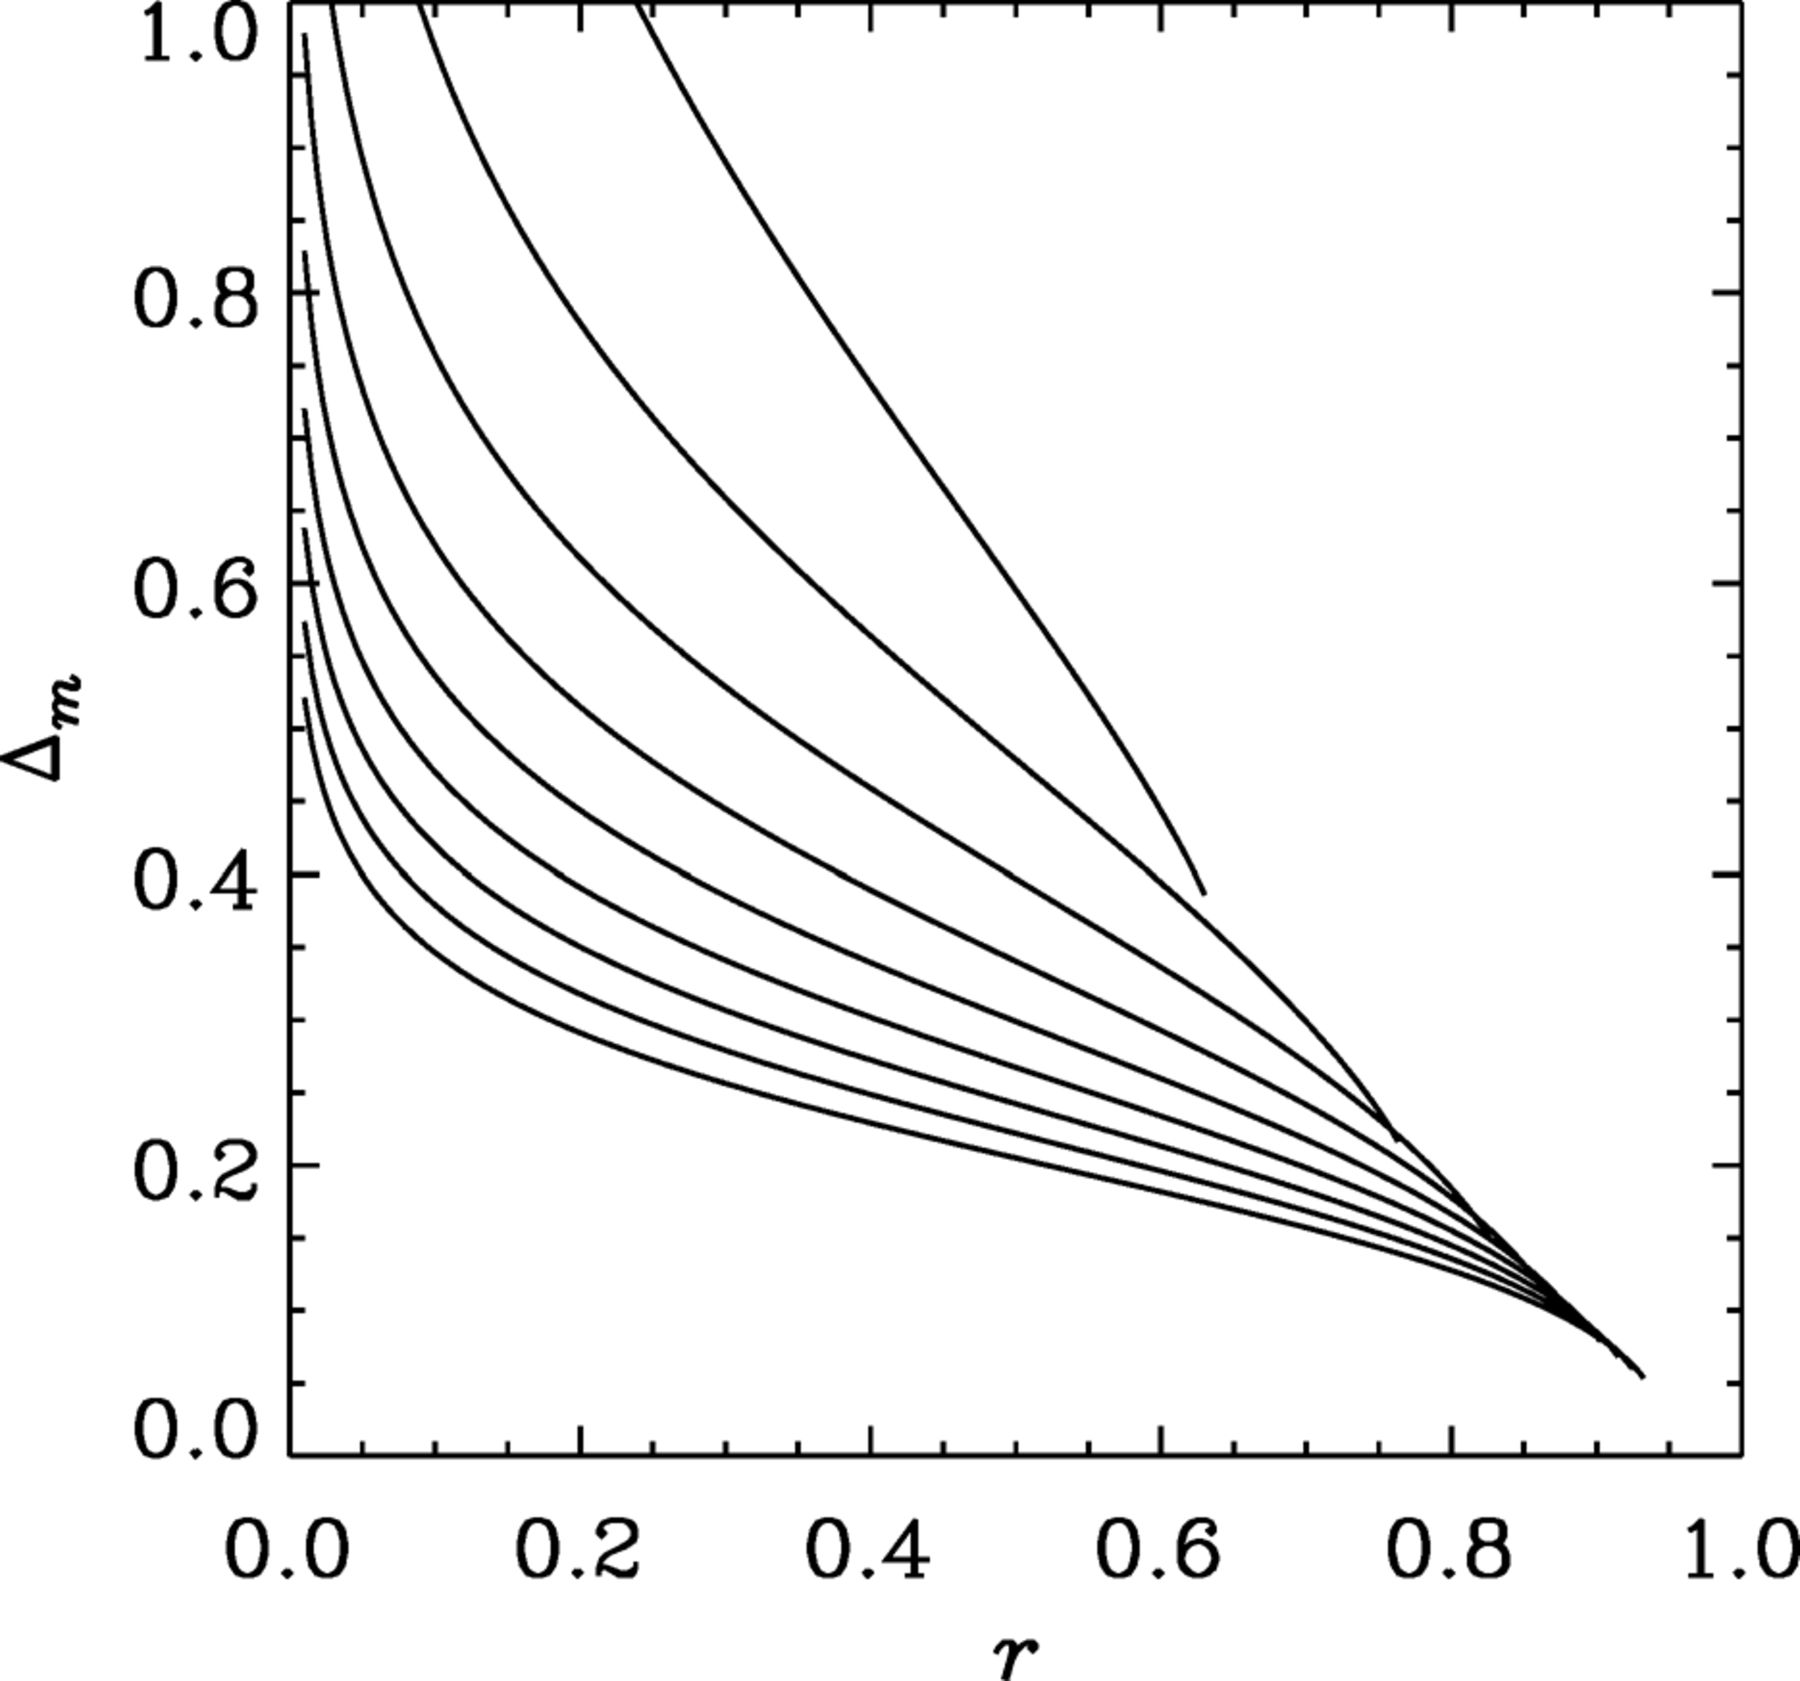
\includegraphics[width=\textwidth]{figures/Delta_m_inner.jpeg}
        %\caption{$y=x$}
        \label{fig:delta_m_inner}
    \end{subfigure}
    \hfill
    \begin{subfigure}[b]{0.49\textwidth}
        \centering
        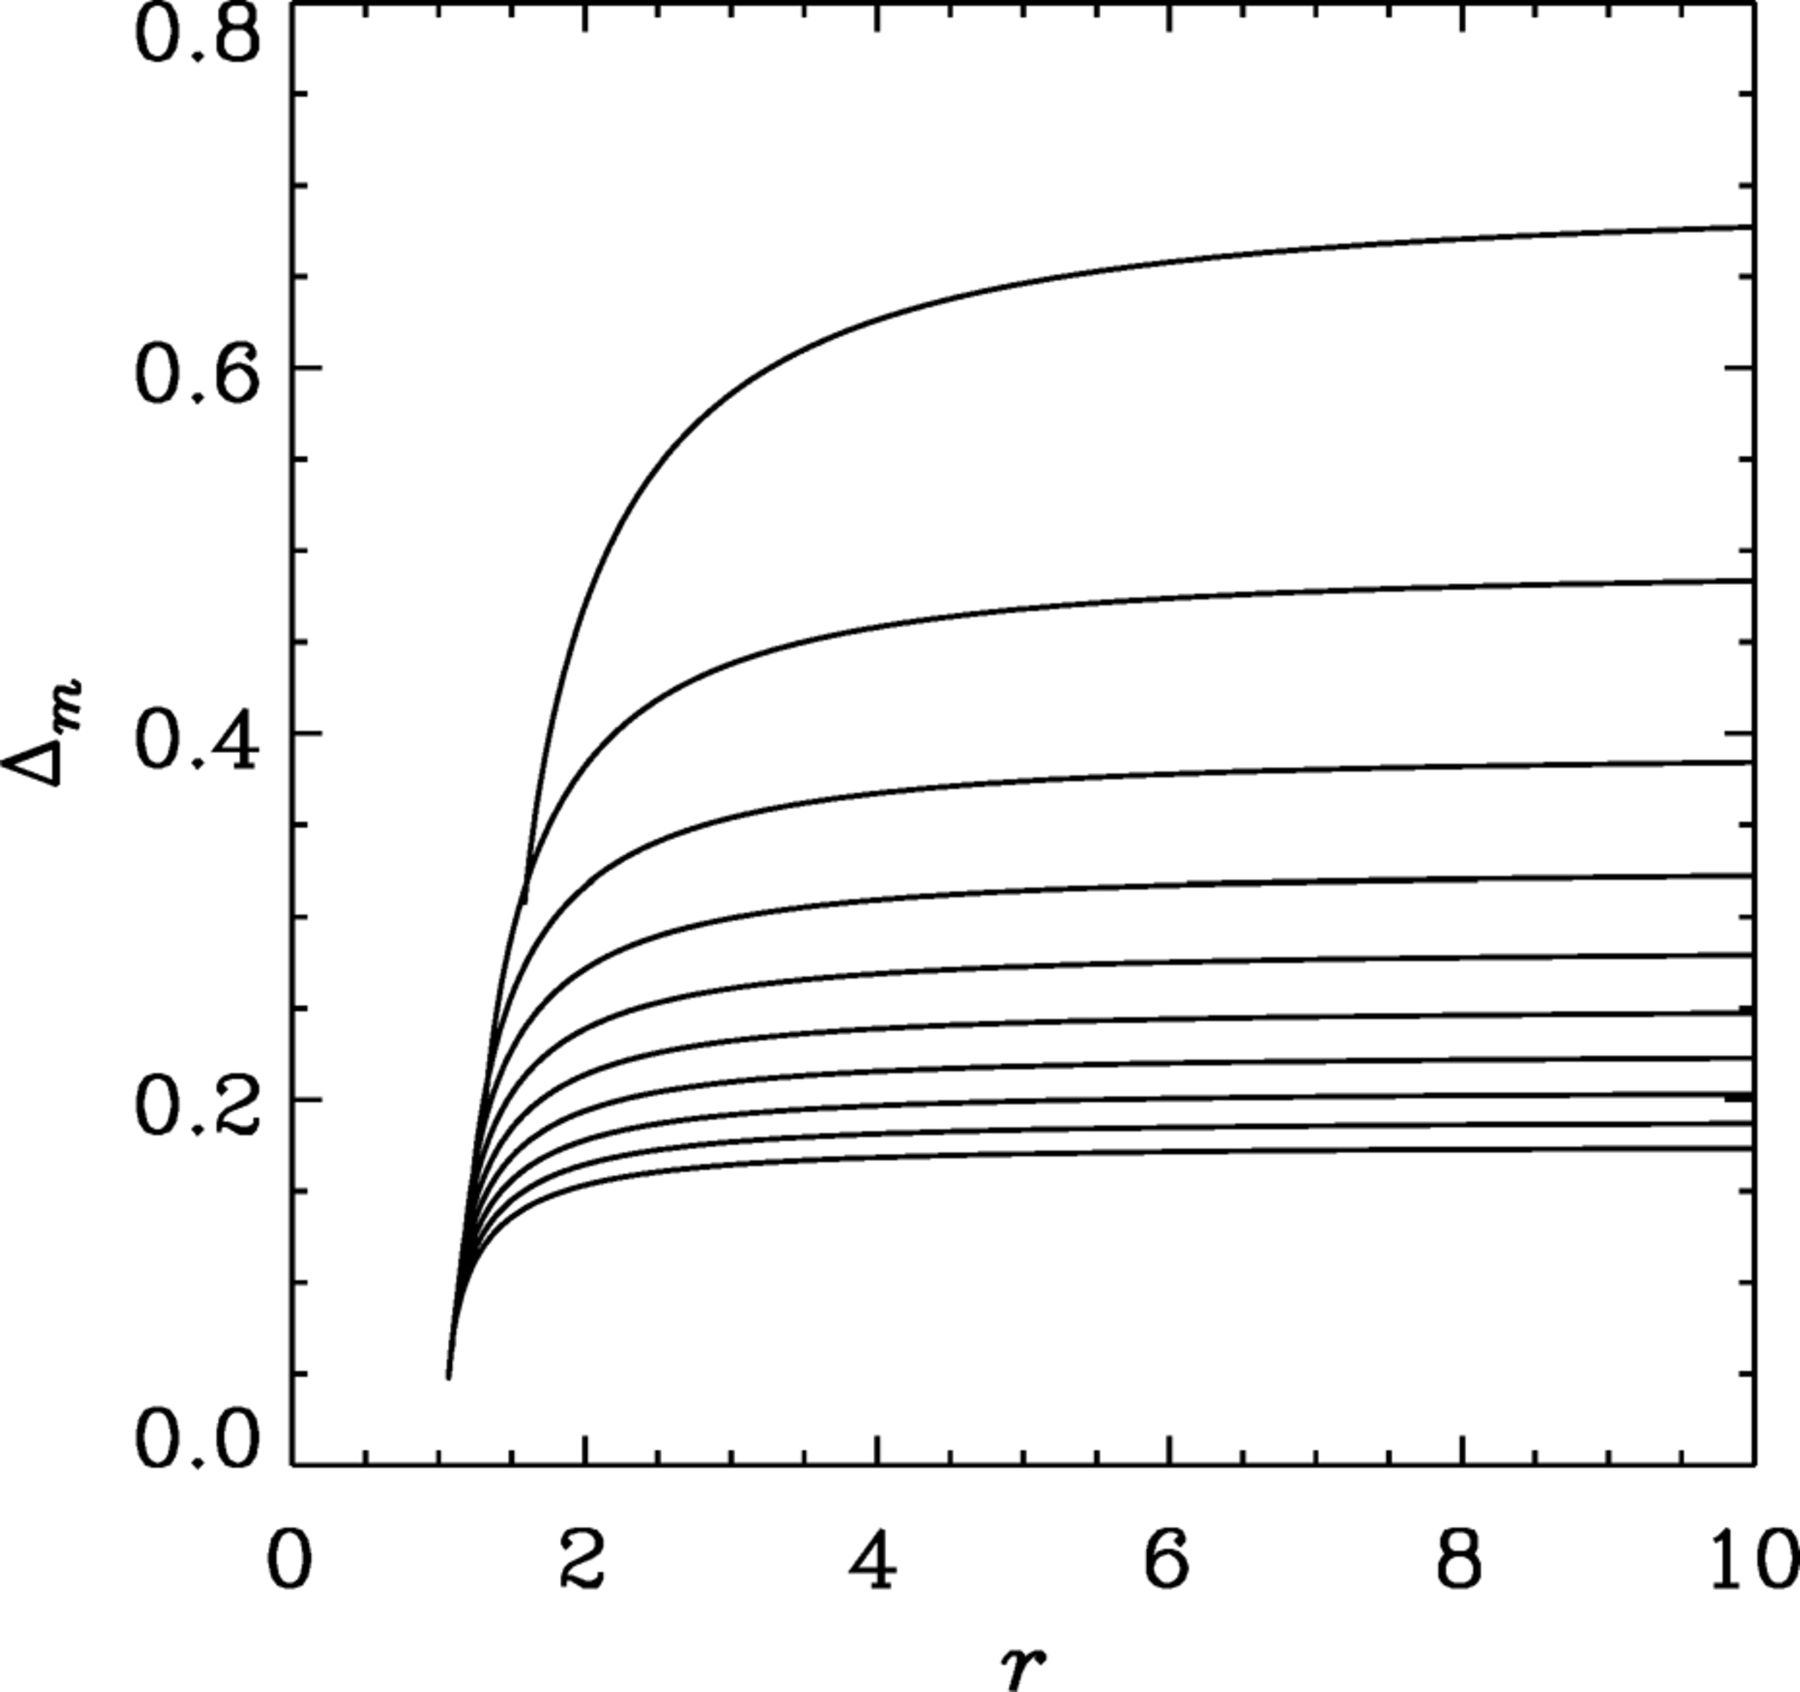
\includegraphics[width=\textwidth]{figures/Delta_m_outer.jpeg}
        %\caption{$y=3sinx$}
        \label{fig:delta_m_outer}
    \end{subfigure}
       \caption{The error in the phase $\Delta_m$ resulting from neglecting the $m$ dependence in Equation~\eqref{eq:phase}, plotted for both the inner (left) and outer (right) disk \citep{ogilvie2002}.
       The planet is placed at $r=1$. Modes $m=1,...,10$ are shown from top to bottom.
       We see that the approximation improves for large $m$ as expected.}
       \label{fig:delta_m}
\end{figure}

\subsection{Additional spiral arms}

In addition to constructive interference of the $n=0$ components causing the planet wake, it is possible for additional spiral arms to form.
These \textit{secondary} and \textit{tertiary} spiral arms (where the planet wake described in the previous section is the \textit{primary} arm) were first seen in numerical calculations \citep{fung2015} and were not very well understood in the context of linear density wave theory until quite recently \citep{bae2018a,miranda2019a}.
Unlike the primary, these spirals are not centred on the planet position, and are instead generated some distance away in the inner disk.

Figure~\ref{fig:additional_arms} shows the phase of the $n=1$ and $n=2$ components in the inner disk.
We see that unlike for the $n=0$ case, the waves are not launched in the vicinity of the planet, or nearby each other.
However the overall behaviour of the constant offset launching term \eqref{eq:spiral_offset} is the same for non-zero $n$, namely that it becomes smaller as $m$ increases and so the launching phases become closer for larger $m$.
Furthermore, the modes become more tightly wound as $m$ increases, with the second term of \eqref{eq:phase} also losing its $m$ dependence for very large values.
These effects allow the larger $m$ modes launched closer to the planet to catch up to the low $m$ modes.
\citet{bae2018a} first performed this analysis and proposed that this catching up effect is responsible for the generation of secondary and tertiary spirals.
This also provides a natural explanation as to why the additional arms are not centred on the planet, as the interference only becomes coherent after the large $m$ modes have caught up in phase.
Bae and Zhu also found that this effect does not operate in the outer disk, as the difference in phase between small and large $m$ modes becomes constant instead of decreasing.

\begin{figure}
    \centering
    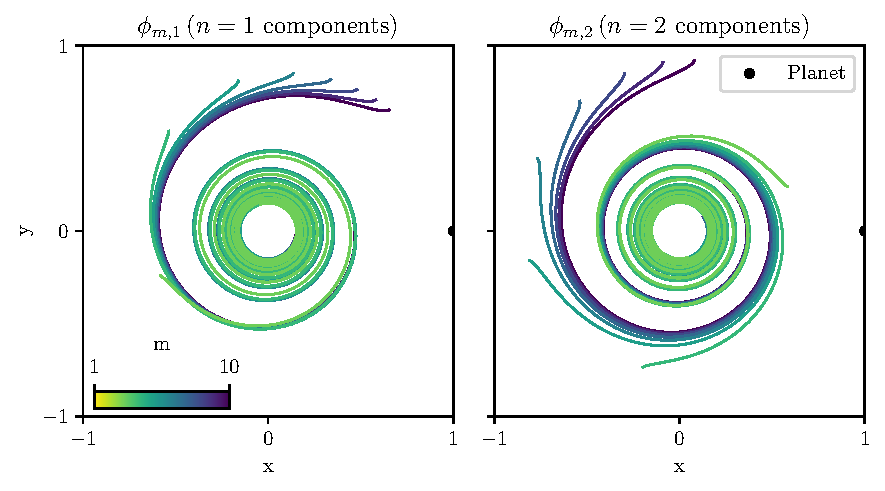
\includegraphics[width = 0.95\textwidth]{figures/inner_n_1_and_2.pdf}
    \caption{Plot of the $n=1$ (left) and $n=2$ spiral arms defined by $\phi_{m,n}$ for modes $m=1,...,10$ (solid lines).
    We show only the inner disk, with the planet placed at $(1,0)$ and disk parameters as in Figure~\ref{fig:wakes_m3}.
    We see that in both the $n=1$ and $n=2$ case, although the spirals start initially out of phase due to different launching positions, the larger $m$ modes are able to catch-up resulting in the formation of the coherent secondary and tertiary spiral arms respectively.}
    \label{fig:additional_arms}
\end{figure}

\citet{miranda2019a} built upon this work through numerical calculations and showed that the formation of additional arms in the inner disk is a robust prediction of the linear theory.
They did this by taking into account the global mode structure outside of the WKB approximation as used in \citet{bae2018a}, and calculated both the phase and amplitude of each mode.
They found that their results in general supported the picture of additional arms resultant from coincident phases, but that taking into account the amplitude information changes the level of correspondence and can be important, especially for the tertiary and higher order arms (those formed by $n>2$).

In this work we will be concerned primarily with the waves generated by the planet in the outer disk and so our models will not include any of the additional arms in the inner disk, only the primary planet wake.

\section{Linear Planet Wake Excitation} \label{sec:linear_wake_excitation}

We now move on to calculating the density and velocity perturbations in the vicinity of the planet due to the planet wake.
This follows the method presented in \citet{goodman2001,rafikov2002a}, which itself is based on the seminal work by \citet{goldreich1978,goldreich1980}.
This involves calculating the linear disk response for each of the Fourier modes of the perturbations.
The solutions are \textit{global} since the WKB approximation is not used.
Historically the interest was first in calculating the Lindblad torque and not the profile of the wake itself, and so the phases of the Fourier harmonics were neglected \citep{goldreich1978,goldreich1980,artymowicz1993a,ward1997}.
\citet{goodman2001} included these phases to solve directly for the shape of the wake.
Their approach for calculating the wake structure splits the problem into two separate regimes: 
\begin{enumerate}
    \item Linear wake \textit{generation}: Provided that $M_{\rm p}$ is not too large ($\lesssim M_1$ defined in Equation~\eqref{eq:char_mass}), the disturbance of the planet nearby the planet is weak enough that the wake can be calculated from linear theory.
    \item Non-linear wake \textit{propagation}: As the wave travels away from the planet it steepens into a shock and non-linear behaviour becomes important.  
\end{enumerate}
This approach is agnostic to the rotation, density and sound speed profiles of the disk, assuming only that they are functions of radius.
It is also assumed that the disk is locally polytropic (see Section~\ref{sec:velocity_perts}), inviscid, and non-self-gravitating.

It should be noted that the used of the language ``generation'' and ``propagation'' are slightly misleading.
The solution that we will calculate is mathematically a steady-state and has no time dependence.
In a physical sense the language is correct; waves are excited nearby the planet before propagating out into the disk.
In a mathematical sense the language is potentially confusing since the solution is independent of time.
These two opposing points of view are reconciled by considering that we are working in the frame where the planet is stationary. 
In reality the spiral pattern is \textit{not} stationary.
The remainder of this section is dedicated to outlining the linear wake generation, while the following section describes the non-linear propagation.

Above we stated that nearby the planet the disturbance is weak enough that linear theory is sufficient to describe wake generation provided the planet is not too large.
This certainly seems counter-intuitive at first glance, should the disturbance not be largest in the direct vicinity of the planet?
This is explained by the fact that a stationary perturber cannot excite density waves in a subsonic flow \citep{landau1959}.
Thus no waves are generated within some characteristic distance from the planet, an effect known as the \textit{torque cut-off} \citep{goldreich1980}.
In a Keplerian disk this distance is $2H_{\rm p}/3$ (see equation \ref{eq:mach1_len}).
The Lindblad resonances within this region, where $m$ is large, are suppressed and therefore contribute minimally to the torque.
In addition the resonances with very low $m$ are not effectively excited due to their distance from the planet.
Indeed the dominant mode is of order $(H_{\rm p} / r_{\rm p})^{-1}$, as mentioned in Section~\ref{sec:planetwake}.
The resonances excited most efficiently are therefore located a few $H_{\rm p}$ from the planet, far enough to justify the linear approach.

\begin{figure}
    \centering
    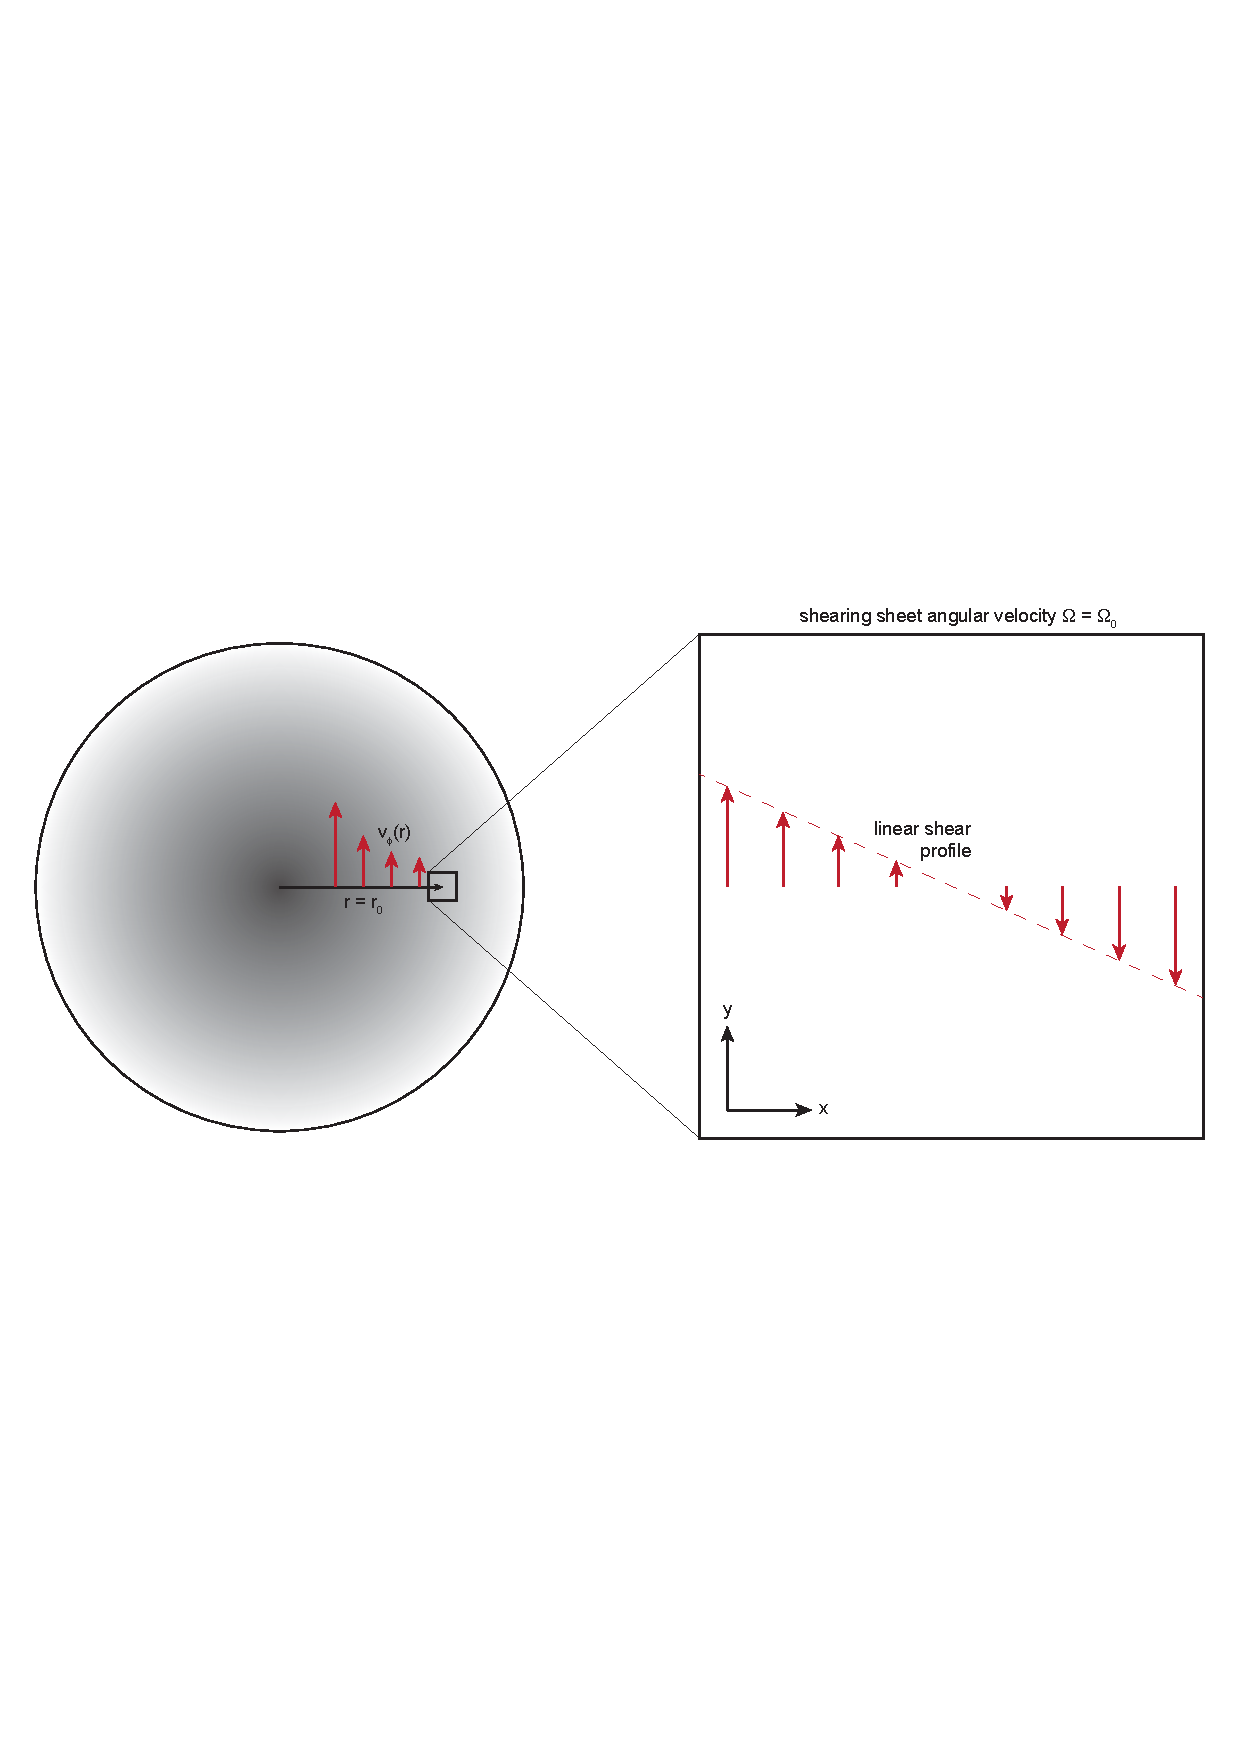
\includegraphics[width = 0.95\textwidth]{figures/shearing_sheet.pdf}
    \caption{Schematic diagram of the shearing-sheet approximation from the lectures notes by \citet{armitage2022}, where in our case $r_0 = r_{\rm p}$ and $\Omega_0 = \Omega_{\rm p}$ and so the shearing box is centred on the planet location.
    Under the approximation the shear nearby the planet is taken to be linear, while the surface density and sound speed are taken to be constant.}
    \label{fig:shearing_sheet}
\end{figure}

The rest of this subsection directly follows \citet{goodman2001}. 
The linear calculation is performed in the \textit{shearing-sheet approximation} \citep{hill1878,goldreich1965}.
This involves defining pseudo-cartesian coordinates centred on the planet location
\begin{align}
    x &= r - r_{\rm p}, \label{eq:local_x} \\
    y &= r_{\rm p} \left( \phi - \phi_{\rm p} \right), \label{eq:local_y}
\end{align}
where $\phi_{\rm p}$ is the azimuthal location of the planet.
The differential rotation of the disk is then expanded to lowest order in $x/r_{\rm p}$, which reduces the azimuthal component of the flow to
\begin{align}
    v_0 = 2 A x; \qquad 2A \equiv r \left. \frac{d \Omega}{dr} \right|_{r_{\rm p}},
\end{align}
where the shear $A$ and rotation $\Omega$ rates are treated as constant (that does \textit{not} make the above derivative zero), as is the vorticity $B \equiv A+\Omega$.
The unperturbed surface density $\Sigma_{\rm p}$ and sound speed $c_{\rm p}$ are also assumed to be constant.
A diagrammatic overview of the shearing-sheet approximation is presented in Figure~\ref{fig:shearing_sheet}.

We adopt as a length unit the Mach-1 length $l_{\rm p}$, which is the distance from the planet where the flow becomes supersonic.
This requires that $v_0 = 2|Ax| > c_{\rm p}$ and so 
\begin{align}
    l_{\rm p} \equiv c_{\rm p} / |2A|. \label{eq:mach1_len}
\end{align}
For the planet mass we adopt the unit
\begin{align}
    M_1 \equiv \frac{c_0^3}{|2A|G}. \label{eq:char_mass}
\end{align}
For a Keplerian disk $M_1$ is equal to the \textit{thermal mass} defined in Equation~\eqref{eq:thermalmass}.
For $M_{\rm p} \gtrsim M_1$ the Roche lobe of the planet will become larger than $l_{\rm p}$, causing the linear approximation to fail.
This is also the gap opening condition for an inviscid disk as discussed in Section~\ref{sec:gap_opening}.
In the linear regime the amplitude of the wake is directly proportional to the planet mass, and so it is sufficient to carry out the calculation only once and scale it appropriately as needed.

In the frame of the planet the wake is stationary such that the radial velocity, azimuthal velocity and density perturbations, $u, v$ and $\sigma = \delta \Sigma / \Sigma$ respectively, are independent of time.
The spatial Fourier transform of these components $\hat{u}, \hat{v}, \hat{\sigma}$ are functions of the coordinate wavenumbers $k_x$ and $k_y$, and they satisfy \citep{goldreich1978,goldreich1980}
\begin{align}
    \frac{d^2 \hat{v}}{d \tau^2} + \left[ c^2 k^2 + \kappa^2 \right]\hat{v} &= -i k_y \frac{d \hat{\Phi}_{\rm p}}{d\tau} + 2i k_x B \hat{\Phi}_{\rm p} \label{eq:fourier_v} \\
    \hat{u} &= - \frac{1}{c^2 k_y^2 + 4 B^2} \left( 2 B \frac{d \hat{v}}{d\tau} - c^2 k_x k_y \hat{v} + 2iBk_y \hat{\Phi}_{\rm p} \right) \label{eq:fourier_u} \\
    \hat{\sigma} &= \frac{i}{c^2 k_y^2 + 4 B^2} \left( k_y \frac{d \hat{v}}{d \tau} + 2B k_x \hat{v} + i k_y^2 \hat{\Phi}_{\rm p} \right), \label{eq:fourier_sigma}
\end{align}
where
\begin{align}
    \tau \equiv -\frac{k_x}{2 A k_y},
\end{align}
is a pseudo-time variable, $k=\sqrt{k_x^2 + k_y^2}$ is the instantaneous wavenumber, and $\hat{\Phi}_{\rm p}=-2\pi G M_{\rm p} / k$ is the Fourier transform of the planet potential.
This system of ordinary differential equations, combined with the initial condition that $\hat{v}=0$ as $\tau \rightarrow - \infty$, constitute a determined system where the unique solution provides the density and velocity perturbations along the wake after Fourier transforming back to coordinate space.

\section{Non-Linear Planet Wake Evolution} \label{sec:nonlinear_evolution}

\citet{goodman2001} first studied the non-linear evolution of the planet wake, neglecting both the disk geometry and variations in density and sound speed, while \citet{rafikov2002a} updated the analysis to include these effects.
We are obviously interested in accounting for these aspects and so we will largely follow \citet{rafikov2002a} in this section, but we will endeavour to make it clear when a result is originally from \citet{goodman2001}.

After the wake is generated, it propagates away from the planet.
At distances $\gg l_{\rm p}$ the contribution of the planet potential becomes negligible.
However unlike in the shearing sheet, we must now consider the evolution of $\Sigma$ and $c$ with radius, as well as the global geometry of the disk.
Rewriting the 2D inviscid fluid Equations \eqref{eq:mom_eq_u}-\eqref{eq:cont_2d} in a rotating frame such that the planet is stationary at $\phi=\phi_{\rm p}$, and $\phi$ is defined such that $\Omega>0$, we obtain \citep{landau1959}
\begin{align}
    &v_r \partial_r v_r + \frac{v_\phi}{r} \partial_\phi v_r - \frac{v_\phi^2}{r} = - \partial_r \Phi - \frac{1}{\Sigma} \partial_r P + 2 \Omega_{\rm p} v_\phi + \Omega_{\rm p}^2 r, \label{eq:mom_eq_u_pl} \\ 
    &v_r \partial_r v_\phi + \frac{v}{r} \partial_\phi v_\phi - \frac{v_r v_\phi}{r} = - \frac{1}{r} \partial_\phi \Phi - \frac{1}{r\Sigma} \partial_\phi P - 2 \Omega_{\rm p} v_r, \label{eq:mom_eq_v_pl} \\
    &\frac{1}{r} \partial_r (r \Sigma v_r) + \frac{1}{r} \partial_\phi (\Sigma v_\phi) = 0,
    \label{eq:cont_2d_pl}
\end{align}
where we have also dropped all time dependence, and $\Phi=\Phi_\star$ since we are neglecting the planet potential.

We now perform a perturbative study including weak non-linear behaviour.
We rewrite the velocities as 
\begin{align}
    v_r = u; \quad v_\phi = v_0(r) + v,
\end{align}
where
\begin{align}
    v_0(r) = r \Delta \Omega \equiv r \left( \Omega - \Omega_{\rm p} \right).
\end{align}
$u$ and $v$ are thus the radial and azimuthal velocity perturbations.
We assume that the shock formed is weak (we will refer to this as the \textit{weak shock approximation}) such that $|u|,|v| \ll |v_0|$. 
$\Delta \Omega \neq 0$ since we are working in region away from the planet.
In addition, the WKB approximation is applied such that $v \ll u$ and $\partial_\phi \ll r \partial_r$ as shown in the appendix of \citet{rafikov2002a}.
With the above considerations, Equations \eqref{eq:mom_eq_u_pl} - \eqref{eq:cont_2d_pl} are transformed to 
\begin{align}
    &\Delta \Omega \partial_\phi u + u \partial_r u - 2 \Omega v = - \frac{1}{\Sigma} \left( \partial_r P - \partial_r P_0  \right) + \frac{v^2}{r}, \label{eq:weak_pert_1} \\
    &\Delta \Omega \partial_\phi v + u \partial_r v + 2Bu = - \frac{1}{r} \left( \frac{1}{\Sigma} \partial_\phi P +u v \right), \label{eq:weak_pert_2} \\
    &\Delta \Omega \partial_\phi \Sigma + u \partial_r \Sigma + \Sigma \partial_r u = - \frac{1}{r} \left( \Sigma u + v \partial_\phi \Sigma + \Sigma \partial_\phi v \right). \label{eq:weak_pert_3}
\end{align}
We have kept terms up to second order in $u$ and $v$.
The radial coordinate $\xi$ is now introduced, consisting of an integral transformation that essential encodes the differential rotation of the disk and simplifies the spatial propagation of the wake (note the similarity to Equation~\eqref{eq:planet_wake}).
It is defined by
\begin{align}
    \xi = \int_{r_{\rm p}}^ r \left[ \Omega(r') - \Omega_{\rm p} \right] \, dr',
\end{align}
and results in the transformation of the Equations \eqref{eq:weak_pert_1} - \eqref{eq:weak_pert_3} to
\begin{align}
    &\partial_\phi u + u \partial_\xi u + \frac{1}{\Sigma} \partial_\xi P - \frac{1}{\Sigma_0} \partial_\xi P_0 = \frac{1}{\Delta \Omega r} \left( 2 \Omega r v + v^2 \right), \label{eq:phi_xi_u} \\
    &\partial_\phi v + u \partial_\xi v + \frac{c^2}{\Delta \Omega r \Sigma} \partial_\phi \Sigma = - \frac{1}{\Delta \Omega r} \left( 2 B r u +uv \right), \label{eq:phi_xi_v} \\
    &\partial_\phi \Sigma + u \partial_\xi \Sigma + \Sigma \partial_\xi u = -\frac{1}{\Delta \Omega r} \left( \Sigma u + v \partial_\phi \Sigma + \Sigma \partial_\phi v \right). \label{eq:phi_xi_sigma}
\end{align}
The left-hand side of the equations above are similar to the usual system of equations that describe the motion of a one-dimensional isentropic gas \citep{landau1959}, except that we have an azimuthal coordinate $\phi$ in place of the time coordinate $t$ and the $\xi$ coordinate in place of the spatial coordinate $x$.
We exploit this similarity to simplify the above equations using the \textit{method of characteristics}.
the 1D isentropic gas flow system possesses two \textit{Riemann invariants} that are each conserved along a curve in the $xt$ plane.
These curves are called the \textit{characteristics}.
This is reviewed briefly in appendix \ref{appendix:isentropic_riemann}.
In our case the non-zero right-hand sides of the equations causes the Riemann invariants $R_\pm$ to no longer be conserved exactly along each of the characteristics $C_\pm$.
Instead, $R_\pm$ evolve in a predictable manner.
Following similar analysis to that in appendix \ref{appendix:isentropic_riemann}, we find that Equations \eqref{eq:phi_xi_u} and \eqref{eq:phi_xi_sigma} reduce to 
\begin{align}
    \begin{split}
        \left[ \partial_\phi + (u \pm c) \partial_\xi \right] R_\pm = - &\left( \frac{1}{\Sigma} \partial_\xi P - \frac{1}{\Sigma_0} \partial_\xi P_0 - c\partial_\xi \frac{2c}{\gamma-1} \pm cu \frac{\partial_\xi \Sigma}{\Sigma} \mp u \partial_\xi \frac{2c}{\gamma-1} \right) \\
        &+ \frac{1}{\Delta \Omega r} \left( 2\Omega r v + v^2 \mp cu \mp cv \partial_\phi \ln \Sigma \mp c \partial_\phi v \right),
    \end{split}
\end{align}
where the Riemann invariants are
\begin{align}
    R_\pm = u \pm \frac{2c}{\gamma-1},
\end{align}
and the characteristics are
\begin{align}
    C_\pm : \, \frac{d\xi}{d\phi} = u \pm c.
\end{align}
The $C_-$ characteristic follows the planet wake, while the $C_+$ characteristic crosses it \citep{goodman2001}.
Therefore $C_-$ is always in the perturbed region while $C_+$ is predominantly in the unperturbed region.
By assuming that the wake-crossings affect the value of $R_+$ minimally and approximating its value as constant, we find that
\begin{align}
    R_+ = \frac{2 c_0}{\gamma - 1},
\end{align}
everywhere.
Since we are assuming $R_+$ is exactly conserved, this implies
\begin{align}
    u = \frac{2(c_0 - c)}{\gamma -1},
\end{align}
and so 
\begin{align}
    R_- = \frac{2(c_0 - 2c)}{\gamma -1}.
\end{align}
Based on these results it is possible to show that the system further reduces to a simple partial differential equation, the inviscid Burger's Equation~\citep[see appendix A of][]{rafikov2002a}
\begin{align}
    \partial_t \chi - \chi \partial_\eta \chi = 0, \label{eq:burgers}
\end{align}
where $\chi$ is a remapping of the surface density perturbation defined as 
\begin{align}
    \chi &\equiv \frac{\gamma +1}{2} \frac{\Sigma - \Sigma_0}{\Sigma_0} g(r), \label{eq:chi} \\
    {\rm where} \quad g(r) &\equiv \frac{2^{1/4}}{r_{\rm p} c_{\rm p} \Sigma_{\rm p}^{1/2}} \sqrt{\frac{r \Sigma_0 c_0^3}{|\Omega - \Omega_{\rm p}|}}, \label{eq:g}
\end{align}
and the coordinates $t$ and $\eta$ are defined as
\begin{align}
    t(r) &\equiv - \frac{r_{\rm p}}{l_{\rm p}} \int_{r_{\rm p}}^r \frac{\Omega(r') - \Omega_{\rm p}}{c_0(r') g(r')} \, dr', \label{eq:t} \\
    \eta(r,\phi) &\equiv \frac{r_{\rm p}}{l_{\rm p}} \left( \phi - \phi_{\rm p} + \int_{r_{\rm p}}^r \frac{\Omega(r') - \Omega_{\rm p}}{c_0(r')} \, dr'  \right) \label{eq:eta}
\end{align}
where $l_{\rm p}$ is the Mach-1 length \eqref{eq:mach1_len} and $\phi_{\rm p}$ is the azimuthal coordinate of the planet.
The $\eta$ coordinate can be written in a clearer form by comparing the third term with Equation~\eqref{eq:planet_wake}:
\begin{align}
    \eta(r,\phi) &\equiv \frac{r_{\rm p}}{l_{\rm p}} \left( \phi - \phi_{\rm wake} \right), \\
    \rm{where} \quad \phi_{\rm wake} &\equiv \phi_{\rm p} - \int_{r_{\rm p}}^r \frac{\Omega(r') - \Omega_{\rm p}}{c_0(r')} dr'. \label{eq:phi_wake}
\end{align}
Intuitively, $t$ can be thought of a coordinate that travels \textit{along} the wake, while $\eta$ is a rescaled angular coordinate that \textit{crosses} the wake.
%To interpret these results we compare the characteristics with the planet wake.
%If we place the planet in our coordinates at azimuth $\phi_{\rm p}$, then from \eqref{eq:planet_wake} the wake shape is given by 
%\begin{align}
%    \phi_{\rm wake} = \phi_{\rm p} - \int_{r_{\rm p}}^r \frac{\Omega(r') - \Omega_{\rm p}}{c_0(r')} \, dr'. \label{eq:wake_shape_rafikov}
%\end{align}
%In terms of $\xi$ this becomes
%\begin{align}
%    \phi_{\rm wake} &= \phi_{\rm p} - \int_{0}^\xi \frac{1}{c_0(\xi')} \, d\xi', \\
%    \Rightarrow \left. \frac{d \xi}{d \phi} \right|_{\rm wake} &= -c_0,
%\end{align}
%and so we see that $C_-$ follows the wake while $C_+$ crosses it.

\subsection{Wave dissipation}

Burger's equation generically produces shocks from smooth waveforms due to the crossing of characteristics \citep{whitham1999}.
Figure~\ref{fig:wake_profiles_GR01} shows the evolution of the wave profile taken at different $t$ values.
We see that at the edge of the linear regime the waveform is initially smooth.
As the wake evolves away from the planet its amplitude decays but areas above and below $\chi=0$ steepen and form two shocks, one moving in the $+\eta$ direction and one moving in the $-\eta$ direction.
The resultant waveform is called an \textit{N-wave} \citep{landau1959}.
\citet{goodman2001} found numerically that the shock forms at 
\begin{align}
    t_{\rm shock} = t_0 + 0.79 \left( \frac{M_{\rm p}}{M_1} \right)^{-1},
\end{align}
and so more massive planets produce a shock closer to the planet.

\begin{figure}
    \centering
    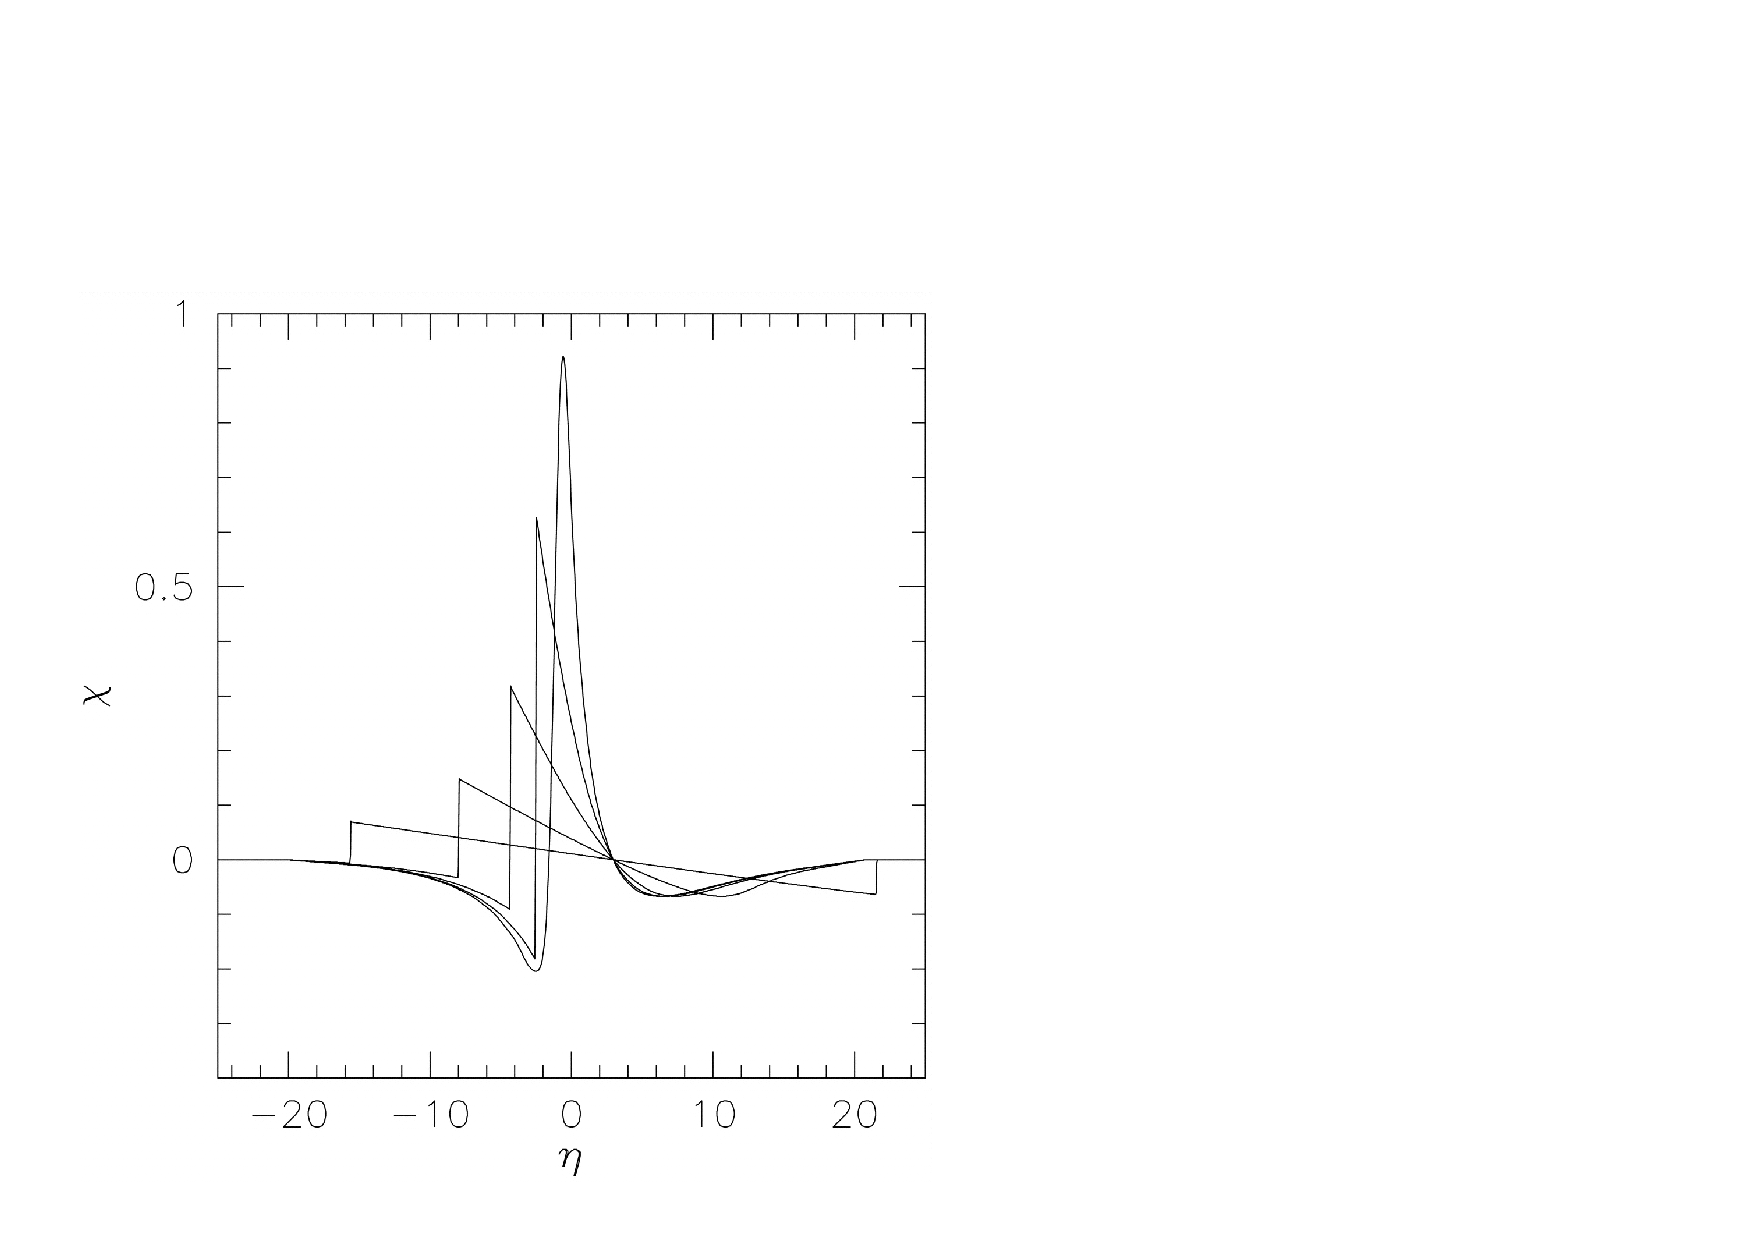
\includegraphics[width = 0.55\textwidth]{figures/wake_profiles_GR01.pdf}
    \caption{Evolution of the wake profile under the Burger's Equation~\eqref{eq:burgers} from \citet{goodman2001}.
    They solved the equation using a second order advection scheme with initial conditions taken from the linear regime at a distance of 2$l_{\rm p}$ from the planet, corresponding to $t=t_0$.
    $\chi$ profiles are shown as slices in $t$ and as a function of $\eta$.
    These profiles were taken at $t-t_0 = 0, 4, 16, 64, 256$ in order of greatest to lowest amplitude.}
    \label{fig:wake_profiles_GR01}
\end{figure}

After the shock is formed the wave becomes dissipative;
its amplitude begins to decay as angular momentum is deposited into the disk.
Prior to shock formation the \textit{angular momentum flux} (AMF), the amount of angular momentum transported along the wake, is perfectly conserved.
The AMF $f_J$ can be calculated as \citep{rafikov2002a}
\begin{align}
    f_J(r) = \frac{c_0^3(r) r}{\Delta\Omega(r)\Sigma_0(r)} \int_0^{2\pi} \left( \Sigma - \Sigma_0 \right)^2 \, d\phi,
\end{align}
which we can rewrite as a function of $t$ using the transformations \eqref{eq:chi}--\eqref{eq:eta} giving
\begin{align}
    f_J(t) &= \frac{2^{3/2} c_{\rm p}^3 r_{\rm p} \Sigma_{\rm p}}{(\gamma + 1)^2 |2 A(r_{\rm p})|} \Phi(t), \\
    \rm{where} \quad \Phi(t) &= \oint \chi^2(t,\eta) \, d\eta 
\end{align}
is the dimensionless AMF, which we will always write as a function of $t$ to avoid confusion with the potential.
After shock formation the resultant dissipation results in the non-conservation of the AMF, as shown in Figure~\ref{fig:AMF}.

Recently \citet{cimerman2021} performed a numerical study to validate the weakly non-linear wake evolution theory.
They compared the Burger's equation evolution with hydrodynamical simulations performed with the grid code \textsc{athena++} \citep{stone2020}.
They found that the transformation to $t,\eta,\chi$ space performs well for a range of planet masses, but also that Burger's equation actually overestimates the wave damping.
This effect however was less severe for larger planet masses.
They also found that it is relatively straightforward to calibrate the theory to account for this discrepancy.
See in particular Sections 5.1, 5.2 and 8.1 of \citet{cimerman2021} for greater detail.
\begin{figure}
    \centering
    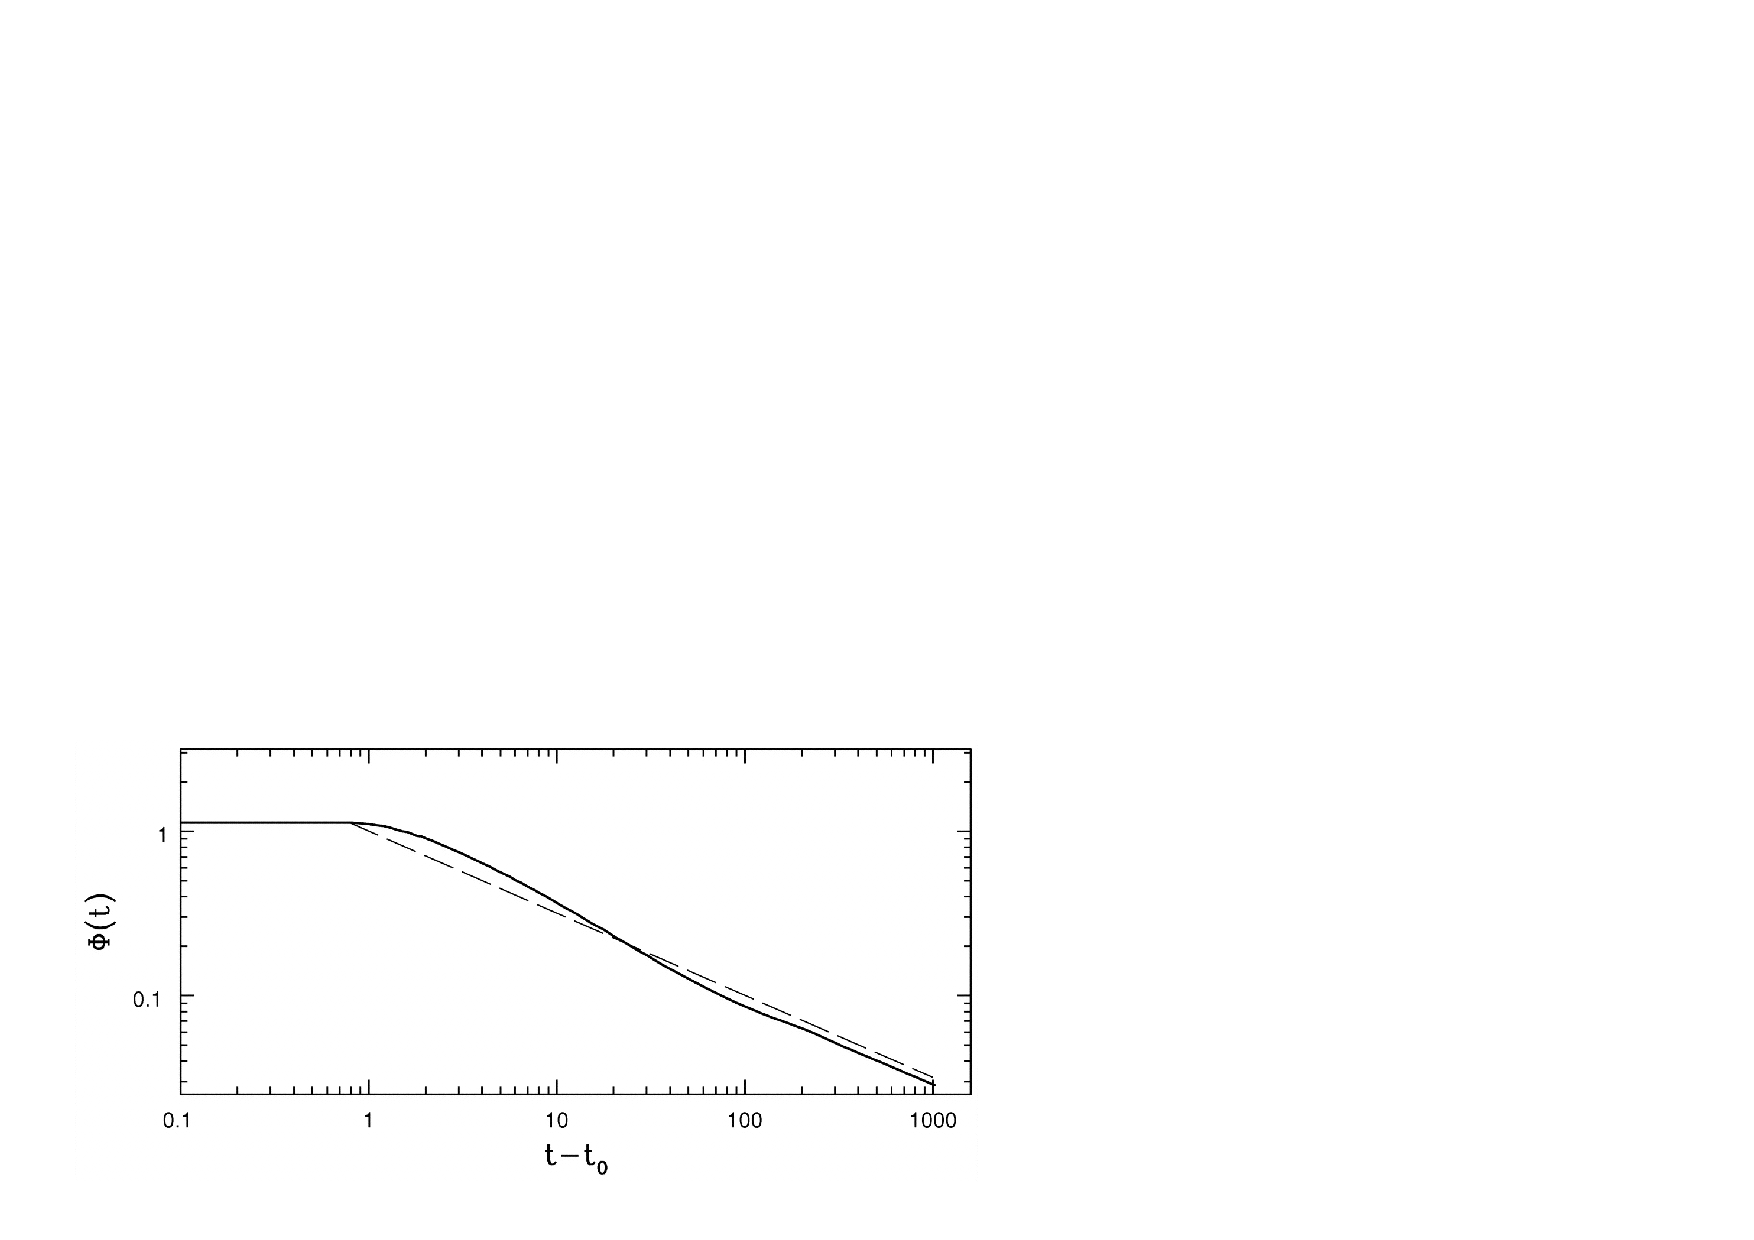
\includegraphics[width = 0.75\textwidth]{figures/AMF_burgers.pdf}
    \caption{Behaviour of the dimensionless AMF $\Phi(t)$ in the non-linear regime as a function of $t$ using $M_{\rm p} = M_1$ \citep[solid line;][]{rafikov2002a}.
    Before the shock is formed at approximately $t-t_0=1$ we see that $\Phi(t)$ is conserved, while decaying steadily after the shock is formed.
    The dashed line demonstrates that the AMF asymptotically scales as $\Phi(t) \propto t^{-1/2}$.
    }
    \label{fig:AMF}
\end{figure}

\subsection{Asymptotic planet mass scaling} \label{sec:asymptotic_N_wave}

While the AMF is no longer conserved in the dissipative wake evolution regime, Burger's equation does encode the perfect conservation of a quantity both before and after shock formation, which is the area under the curve $\chi$ \citep{landau1959,whitham1999}.
We will show that physically this corresponds to conservation of mass in the disk.
The area $\mathcal{A}$ under the curve at a ``time'' $t$ is given by
\begin{align}
    \mathcal{A} = \oint \chi \, d\eta = \frac{(\gamma + 1)g(r)r_{\rm p}}{2 \Sigma_0 l_{\rm p}} \int_0^{2\pi}  \left( \Sigma - \Sigma_0 \right) \, d\phi, 
\end{align}
where in the second equality we have used transformations \eqref{eq:chi} and \eqref{eq:eta}.
The second integral in the above must evaluate to zero by physical argument, since the perturbed density profile must have the same mass as the unperturbed profile $\int_0^{2 \pi} \Sigma \, d\phi = \int_0^{2 \pi} \Sigma_0 \, d\phi$.
Therefore the conservative properties of Burger's equation, that $\frac{d\mathcal{A}}{dt}=0$, ensures that the mass of each annulus in the disk is unchanged by the density perturbation.

Using this area conservation property \citet{bollati2021} derived an asymptotic solution for the N-wave profile of the planet wake in the limit of $t\rightarrow\infty$:
\begin{align}
    \chi(t, \eta) \sim \begin{dcases}
        \frac{\rm{sgn}\left(r - r_{\rm p}\right) \eta + \tilde{\eta}}{t - t_0} \quad &\rm{if} \, \eta \in \left[\eta_-, \eta_+ \right], \\
        0 \quad &\rm{else},
    \end{dcases}
\end{align}
where $\tilde{\eta} \simeq 2.96$ is the value of $\eta$ where the N-wave intersects the $\eta$-axis.
Additionally
\begin{align} 
    \eta_\pm &= - \rm{sgn}(r - r_{\rm p}) \tilde{\eta} \pm \sqrt{2 \mathcal{A} (t - t_0)}, \\
    \rm{where} \quad \mathcal{A} &= |C_0| \frac{\gamma + 1}{2^{3/4}} \frac{M_{\rm p}}{M_1},
\end{align}
and $C_0 \simeq -0.4$ is a numerically determined constant \citep{bollati2020}.

From this asymptotic solution one may determine a scaling relation for the planet mass in terms of only the distance the wake has propagated from the planet $t-t_0$ and the width of the wake $\eta_+ - \eta_-$, given by 
\begin{align}
    \frac{M_{\rm p}}{M_1} \propto \frac{\left( \eta_+ - \eta_- \right)^2}{t - t_0}. \label{eq:Mp_propto}
\end{align}
This scaling relation tells us the fundamental information that must be determined in order to constrain a planet mass from its wake observationally.
We see that we must know the reference mass $M_1$, as well as the transformations $t(r)$ and $\eta(r,\phi)$.
From this we may use Equations \eqref{eq:char_mass}, \eqref{eq:t} and \eqref{eq:eta} to produce a full list of basic quantities of the disk and planet system that must be determined:
\begin{enumerate}
    \item The rotation profile of the disk $\Omega(r)$ (although Keplerian is likely a good approximation),
    \item The unperturbed sound speed profile $c_0(r)$ OR the pressure scale height $H(r)$,
    \item The unperturbed surface density profile $\Sigma_0(r)$,
    \item The planet orbital radius $r_{\rm p}$,
    \item The planet azimuth $\phi_{\rm p}$.
\end{enumerate}
However, we note that from Equation~\eqref{eq:phi_wake} that $c_0(r)$, $r_{\rm p}$ and $\phi_{\rm p}$ are all determined by the shape of the wake.
Therefore if we assume a disk to be Keplerian and fit the wake shape, all that remains is to determine $\Sigma_0$ and then $M_{\rm p}$ will be determined.
The most straightforward way to constrain this is through determining the size of the perturbation in $\chi$ which depends on $g(r)$ and so on $\Sigma_0$.
While at this stage it is not clear on how to extract the information from observations, this at least shows that the planet mass is determined entirely by the wake shape and amplitude.

Finally, while it is possible to calculate the scale factor for the proportionality relation \eqref{eq:Mp_propto} from theory, the work of \citet{cimerman2021} suggests that this is better done through comparison with hydrodynamical simulations.

\section{Gap Opening} \label{sec:gap_opening}

For sufficiently large planets, the non-linear effects are such that the planet wake shocks immediately after formation and the solution can no longer be neatly separated into the linear generation and non-linear propagation regimes.
As already hinted at, the condition under which this occurs in an inviscid disk is that the planet mass $M_{\rm p}$ exceeds the characteristic mass $M_1$ defined in Equation~\eqref{eq:char_mass}.
For a Keplerian disk the minimum gap-opening mass is the thermal mass \citep{lin1993}, defined as \citep{goodman2001}
\begin{align}
    M_{\rm th} \equiv \frac{2}{3} \left( \frac{H_{\rm p}}{r_{\rm p}}  \right)^3 M_\star. \label{eq:thermalmass}
\end{align}
Thus the wake solution approach presented in Sections \ref{sec:linear_wake_excitation} and \ref{sec:nonlinear_evolution} is only \textit{strictly} valid for sub-thermal mass planets. It is not clear however, that the non-linear Burger's equation evolution is invalid for planets greater than the thermal mass. The non-linear evolution prescription's strictest requirement is that the shock is sufficiently weak, such that the perturbative approach is still valid.

Gap opening occurs because the dissipative shock fronts allow angular momentum from the material nearby the disk to be deposited elsewhere \citep{lin1979,goldreich1979,goldreich1980}.
The rough physical criterion for a gap to open depends on two conditions.
Firstly the Hill radius of the planet $r_{\rm H}$ \citep{hill1878} must fulfil $r_{\rm H} \gtrsim H$, known as the \textit{thermal condition}.
Secondly the transfer rate of angular momentum between the wake and disk must exceed the local transport rate from effective viscosity \citep{lin1993}.
The thermal condition is equivalent to $M_{\rm p} = M_{\rm th}$ while the second is irrelevant to discussions of inviscid disks.

\citet{kanagawa2015} found an analytic relation between planet mass $M_{\rm p}$, central star mass $M_*$, viscosity $\alpha$ \citep{shakura1973}, and gap depth $\Sigma_{\rm p} / \Sigma_0$ in the case of an axisymmetric and geometrically thin gas disk subject to viscous evolution
\begin{align}
    \frac{M_{\rm p}}{M_\star} = 5 \times 10^{-4} \left( \frac{\Sigma_0}{\Sigma_{\rm p}} - 1 \right)^{\frac{1}{2}} \left( \frac{(H/r)_{\rm p}}{0.1}  \right)^{\frac{5}{2}} \left( \frac{\alpha}{10^{-3}} \right)^{\frac{1}{2}}, \label{eq:kanagawa_gap_depth}
\end{align}
where the gap depth $\Sigma_{\rm p} / \Sigma_0$ is written in terms of the surface density in the gap $\Sigma_{\rm p}$, and the unperturbed surface density $\Sigma_0$.

The modern understanding of gap opening, considering both the effects of viscosity and non-linear planet wake evolution, states that the thermal condition is unnecessary.
Instead planets $\lesssim M_{\rm th}$ may be capable of opening a gap depending on the disk conditions \citep{rafikov2002}.
The opening criterion is given by \citep{kanagawa2015a}
\begin{align}
    M_{\rm p} \gtrsim 5 \left( \frac{H_{\rm p}}{r_{\rm p}} \right)^\frac{5}{2} \alpha^\frac{1}{2} M_\star.
\end{align}
Hydrodynamical simulations have confirmed the ability of sub-thermal mass planets to open gaps \citep{duffell2013}.

Finally, gap-opening occurs not only in the gas component of disks, but also the dust component.
Dust gaps are actually far more pervasive observationally \citep[e.g.][]{almapartnership2015,andrews2016,isella2016,andrews2018,huang2018b}, since the gas structure of a disk is less straightforward to probe \citep{miotello2022}.
Dust gaps can be created through the mechanisms already discussed, since the grains will migrate to the pressure maxima induced at the edges of the gas gap \citep{paardekooper2004}.
The large and weakly-coupled grains become trapped at these maxima.
Smaller grains couple to the gas strongly and so flow with it into the vicinity of the planet before being accreted \citep{paardekooper2006,fouchet2007}.
Additionally, gaps may be induced only in the dust the component.
Drag acts on dust grains interior and exterior to the planets orbit resulting in inward radial migration.
Exterior to the orbit the tidal torque induced by the planet resists the inward drift
\citep{dipierro2016}.
Dust grains are therefore cleared from near the planets orbit resulting in a dust gap.

    \chapter{Semi-Analytic Models of Planet Wakes}
    \setlength{\headheight}{13.59999pt}

This chapter is concerned with the method that we have used to create semi-analytic models of planet wakes.
These models encompass both the linear and non-linear disk response caused by a perturbing planet as described in the previous chapter. 
This work builds on that presented in \citet{bollati2021} and so we will be predominantly concerned with the differences between our methods.
However we aim to provide enough detail to be understandable without having read the aforementioned paper.
The chapter concludes with an application of the analytics\footnote{We will use the terms analytic and semi-analytic interchangeably from now on.}, where we model the kinematic arc detected in the disk of HD~169142 in order to constrain the mass of a potential embedded planet in the disk.

\section{Wakeflow: A Python Package For Semi-Analytic Models of Planet Wakes} \label{sec:JOSS}

This section has been submitted to the Journal of Open Source Science and is currently in review (\citeauthor{hildersubmitted}, submitted). The preprint is publicly available here: \url{https://github.com/TomHilder/wakeflow/blob/master/paper/paper.md}

\subsubsection{Summary}

\textsc{wakeflow} is a Python package for generating semi-analytic models of the perturbations induced by planets embedded in gaseous circumstellar disks. 
These perturbations take the form of a spiral shock wave \citep{ogilvie2002}, and are often called a ``planet wake'' in analogy with that produced by a boat in a lake.

\subsubsection{Statement of Need}

Detecting newly formed planets embedded in their disk is a challenging problem in the field of planet formation. 
A major area of progress in recent years is the detection of planets by the gravitationally induced disturbance in their host disks. 
This disturbance, caused by the planet wake, manifests as a deviation in velocity from the bulk flow which may be measured through the Doppler shift of molecular lines \citep[e.g.][]{perez2015, pinte2018a}. 
Such kinematic observations have been accurately reproduced through 3D fluid simulations of the planet-disk interaction, allowing for the inference of planet and disk properties \citep{pinte2018a, pinte2019}. 
However, these studies are computationally expensive.

\textsc{wakeflow} eases this computational cost by applying the theory of planet wake generation and propagation \citep{goldreich1979,goodman2001,rafikov2002a,bollati2021} to create semi-analytic models of planet wakes. 
\textsc{wakeflow} models are readily created in a few seconds on a modern laptop, as opposed to the hours of supercomputer time needed for 3D hydrodynamical simulations. 
The relatively low computational cost of \textsc{wakeflow} means that researchers can get an idea of whether planet-disk interactions can explain their observations, and the disk and planet parameters needed, before spending computer time on more detailed simulations.

\textsc{wakeflow} can interface with the radiative transfer code \textsc{mcfost} \citep{pinte2006,pinte2009} in order to create synthetic observations of the semi-analytic models for direct comparison with observed continuum or line emission.

\textsc{wakeflow} is partially adapted from a previous Python code also written by us called \textsc{analytical\_kinks} \citep{bollati2021a}. 
\textsc{wakeflow} is intended to be a more complete, versatile and easy to use version of that code, and it obeys standard Python packaging conventions.
In addition, \textsc{wakeflow} can directly interface with \textsc{mcfost} while \textsc{analytical\_kinks} cannot.
At the time of writing, no other open source software packages exist to generate the perturbations induced by an embedded planet in a circumstellar disk using the semi-analytic theory of planet wakes.

Existing scientific publications focusing on detecting the kinematic signatures of planets that have used \textsc{wakeflow} or its predecessor \textsc{analytical\_kinks} include \citet{bollati2021}, \citet{calcino2022}, \citet{teague2022}, \citet{garg2022} and \citeauthor{fasanoinprep.} (in prep.).

\subsubsection{Acknowledgements}

\textsc{wakeflow} relies on the following scientific Python packages: \textsc{NumPy} \citep{harris2020}, \textsc{matplotlib} \citep{hunter2007}, \textsc{SciPy} \citep{virtanen2020} and \textsc{Astropy} \citep{astropycollaboration2022}.

\section{Semi-Analytic Solution Algorithm}

\begin{figure}
    \centering
    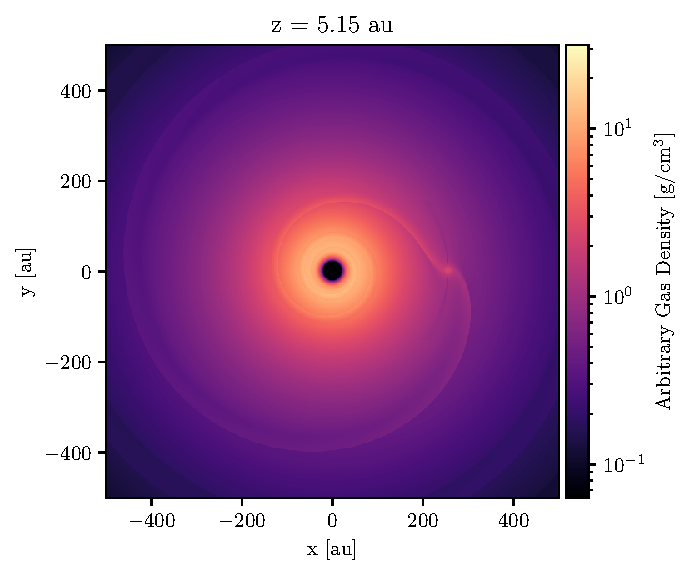
\includegraphics[width = 0.85\textwidth]{figures/wakeflow_tutorial_plot.pdf}
    \caption{Density slice of a \textsc{wakeflow} model at constant height $z=5.15$ au, plotted with a logarithmic colourbar. The model contains a $0.5 \, \mathrm{M_J}$ planet, placed at a separation of $256$ au from the central star. These results were generated following the quickstart tutorial publicly available on the \textsc{wakeflow} documentation\protect\footnotemark, and are meant as a model of the planet wake in the disk of HD~163296, with disk parameters chosen following \citet{pinte2018a} and \citet{calcino2022}.}
    \label{fig:example_model}
\end{figure}

\footnotetext{\url{https://wakeflow.readthedocs.io/en/latest/tutorials/quickstart.html}}

Here we provide an overview of the algorithm used by \textsc{wakeflow} to generate models.
For stages that are sufficiently different to \citet{bollati2021}, further detail will be provided in section \ref{sec:model_considerations}.
The algorithm proceeds as:
\begin{enumerate}
    \item The global grid is generated based on the user's choice of grid geometry and number of grid points. Both cylindrical and cartesian grid geometries are supported, as well as the \textsc{mcfost} grid geometry.
    
    The run time for \textsc{wakeflow} scales linearly in the number of grid points $n_x \times n_y$ or $n_r \times n_\phi$, but is roughly independent of the number of points in the vertical direction $n_z$.
    
    \item The unperturbed disk density and velocity structure is calculated based on the user's choice of disk parameters as outlined in section \ref{sec:diskstruct}.
    
    \item The linear perturbations are calculated and mapped onto the global disk geometry, following section \ref{sec:linear_box}. The perturbations $\sigma, u$ and $v$ are assumed to be independent of vertical height $z$.
    
    \item The initial conditions for the non-linear evolution are extracted from the edge of the linear regime along a slice of constant $t$, as described in \ref{sec:transformations}.
    
    \item Burger's equation is solved in $(t,\eta)$ space until $t_{\rm f}=300$ using a vectorised Godunov solver \citep{astrofluids}. Unlike in \citet{bollati2021} we use make use of adaptive time-steps, which both ensures the stability of the solution (especially for large planet masses that shock quickly), as well as improves efficiency as large time-steps are taken when appropriate. After $t_{\rm f}$, the asymptotic solution is taken as described in \citet{bollati2021}.
    
    \item The solution $\chi(t,\eta)$ is transformed to $\chi(r,\phi)$ as described in section \ref{sec:transformations}.
    
    \item The density perturbations in the non-linear regime are calculated from $\chi$ using equations \ref{eq:chi} and \ref{eq:g_power}. The velocity perturbations are calculated from $\chi$ as described in section \ref{sec:velocity_perts}. Again, all perturbations $\sigma, u$ and $v$ are assumed to be independent of $z$.
    
    \item The results are written to the disk. This output may be a \textit{.fits} file if desired.
\end{enumerate}

\noindent A density slice of an example \textsc{wakeflow} model is shown in Figure \ref{fig:example_model}.
This model was calculated on a $1000 \times 1000 \times 30$ grid in $x,y$ and $z$ respectively, and took in $19.1$ seconds to compute on an Apple M1 processor.

\section{Theoretical and Numerical Considerations} \label{sec:model_considerations}

\subsection{Unperturbed Disk Structure} \label{sec:diskstruct}

Here we outline the unperturbed disk model used in \textsc{wakeflow} onto which the perturbations are added.

\subsubsection{Temperature}

We assume that the sound speed $c$ obeys a simple radial power law 
\begin{align}
    c \propto r^{-q},
\end{align}
where $q$ is some real number. Thus the disk temperature scales as 
\begin{align}
    T \propto c^2 \propto r^{-2q}.
\end{align}
The constant of proportionality for these relations in determined by the user specified value of the disk aspect ratio $H/r$ at $r=r_{\rm ref}$

\subsubsection{Density}

We use a density structure derived by assuming that the disk is in vertical hydrostatic equilibrium \citep{pringle1981}, but unlike in equation \ref{eq:vertical_rho} we will not assume that $z\ll r$.
The density $\rho$ is given by 
\begin{align}
    \rho(r,z) \propto \left( \frac{r}{r_{\rm ref}} \right)^{-p} \exp{\left( \frac{G M_\star}{c^2} \left[ \frac{1}{\sqrt{r^2 + z^2}} - \frac{1}{r} \right] \right)},
\end{align}
where $p$ is some real number. 
The constant of proportionality is set directly by the user, or calculated by \textsc{mcfost} based on the total gas mass.

Very commonly the density profile is parameterised in terms of the surface density $\Sigma$, not the actual density $\rho$ as above.
If the surface density is parameterised as $\Sigma \propto r^{-\delta}$ where $\delta$ is some real number, then equation \ref{eq:surf_dens_to_dens} gives the approximate relation 
\begin{align}
    p \simeq \frac{3}{2} - q + \delta,
\end{align}
which can be used to convert between density parameterisations.
This conversion is only approximate in our context, since is does assume that $z \ll r$ and our density profile does not.
However this turns out not to matter since $\delta$ will only show up in the $t(r)$ mapping which we will assume is the same for all $z$.

\subsubsection{Velocities}

The radial and vertical motions in the unperturbed disk are set to zero. 
The rotation is derived assuming radial force balance \citep[e.g.][]{nelson2013} and is given by 
\begin{align}
    \Omega(r,z) = \Omega_{\rm K} \left[ - \left(p + 2q\right) \left( \frac{H}{r} \right)^2 + \left( 1-2q \right) + \frac{2qr}{\sqrt{r^2 + z^2}}\right]^{1/2}, \label{eq:omega_wf_ps}
\end{align}
where $\Omega_{\rm K}$ is as defined in equation \ref{eq:point_pot}.

\subsection{Linear Box} \label{sec:linear_box}

The solution in the linear regime nearby the planet used in \textsc{wakeflow} was calculated by \citet{bollati2020} and \citet{bollati2021} by solving equations \ref{eq:fourier_v} -- \ref{eq:fourier_sigma} numerically, following the procedure outlined in \citet{goodman2001}.
Here, we simply read their dimensionless calculations and scale them accordingly for our purposes. Figure \ref{fig:lin_box_bollati} shows the $u$ and $v$ solutions presented in \citet{bollati2021}, in local cartesian coordinates $x,y$ centred on the planet location.
The $x,y$ coordinates are scaled by the Mach-1 length $l_{\rm p} = 2H_{\rm p}/3$, while the perturbation are scaled by the planet mass in units of the thermal mass $M_{\rm p} / M_{\rm th}$.

\begin{figure}
    \centering
    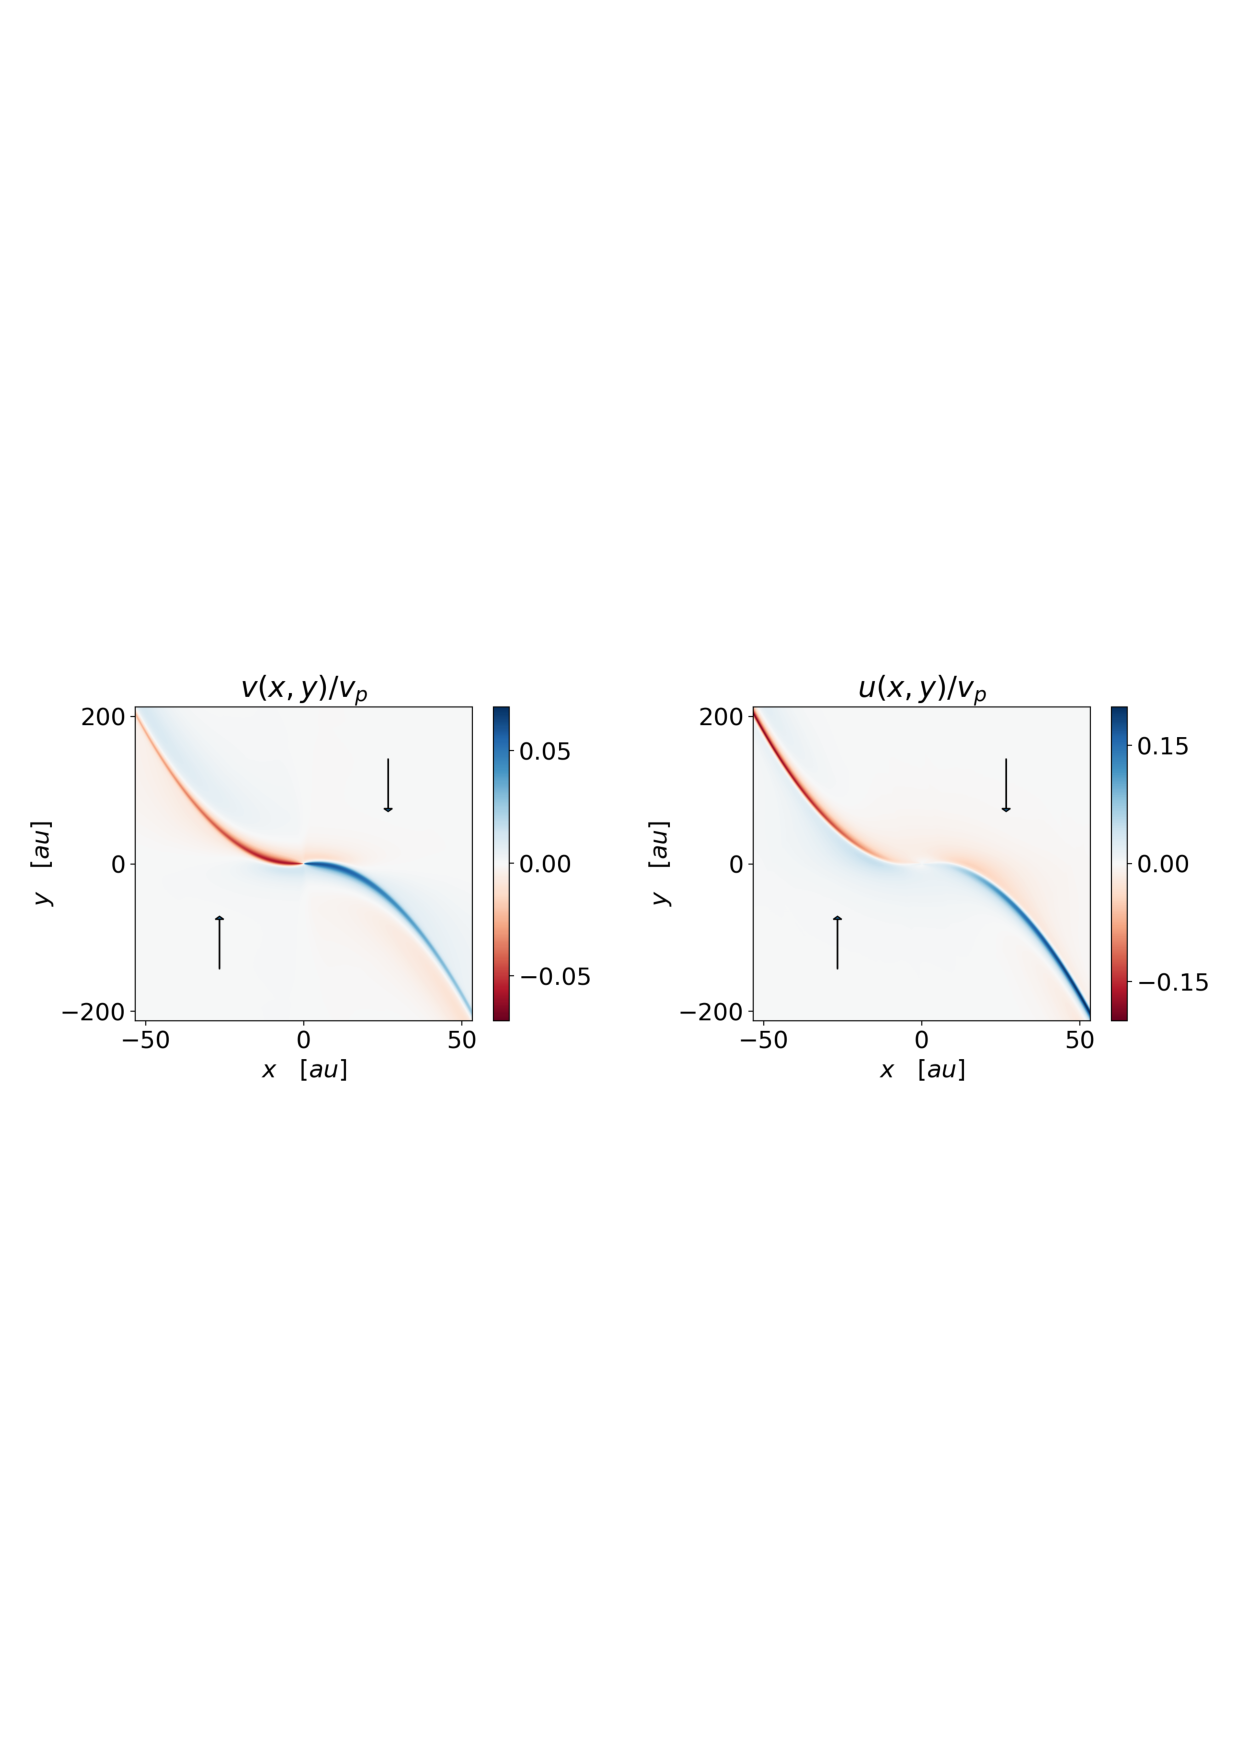
\includegraphics[width = 0.95\textwidth]{figures/linear_box_bollati.pdf}
    \caption{Linear azimuthal (left) and radial (right) velocity perturbations $v$ and $u$ centred on the planet in local cartesian coordinates as defined in equations \ref{eq:local_x} and \ref{eq:local_y}, and calculated by \citet{bollati2021}. The velocity is given in units of $v_{\rm p} = \Omega_{\rm K}(r_{\rm p})$, and the arrows denote the direction of the shearing gas flow in a frame centred on the planet.}
    \label{fig:lin_box_bollati}
\end{figure}

Unlike \citet{bollati2021}, we do not include the linear regime results as a square box in the global solution.
Instead, we take seriously the transformation \ref{eq:local_y}, and interpret $y$ as an arc-length instead of a true Cartesian coordinate, giving us an \textit{annulus segment} instead of a \textit{square box} (we will from now on refer to the former simply as the \textit{linear box}).
Indeed, when the $\chi$ initial condition is extracted from the edge of the box, this is the treatment used for $y$.
It is therefore more honest to take this approach when mapping the linear solution onto the global grid, and has the added benefit of resulting in a more continuous solution.
In addition, we allow for separate variation of the height (angular extent) and width (radial extent) of the box.
This is motivated by considering that the box size was originally chosen as the Mach-1 length through an argument about resonance location (see section \ref{sec:linear_wake_excitation}).
Since these locations are constant as $\phi$ varies, it is perfectly acceptable to extend the linear regime in the angular direction.
The caveat to this is that the linear solution was derived in the shearing sheet approximation where the global geometry of the disk is not considered.
The curvature of the $y$ coordinate becomes more extreme as the box size increases angularly.
By default, \textsc{wakeflow} chooses the angular extent of the box to be the same as the radial extent, with a height of $4H_{\rm p}/3$.

\subsection{Transformations} \label{sec:transformations}

To perform transformation between the physical coordinates and $(t,\eta)$ space in calculating our models, we apply the general forms of the transformations \ref{eq:g} -- \ref{eq:eta} to so-called \textit{power-law disks} where the sound speed and surface density are parameterised as
\begin{align}
    c(r) = c_{\rm p} \left(\frac{r}{r_{\rm p}}\right)^{-q}; \quad \Sigma(r) = \Sigma_{\rm p} \left(\frac{r}{r_{\rm p}}\right)^{-\delta},
\end{align}
where $c_{\rm p}$ and $\Sigma_{\rm p}$ are the sound speed and surface density at $r_{\rm p}$.
Assuming also that $\Omega=\Omega_{\rm K}$, then equation \ref{eq:phi_wake} becomes \citep{rafikov2002a}
\begin{align}
    \phi_{\rm wake}(r) = \phi_{\rm p} + {\rm sgn} \left( r - r_{\rm p} \right) \frac{r_{\rm p}}{H_{\rm p}} \left[ \frac{2}{2q-1} \left(\frac{r}{r_{\rm p}}\right)^{q-\frac{1}{2}} - \frac{1}{q+1} \left(\frac{r}{r_{\rm p}}\right)^{q+1} - \frac{3}{\left(2q-1\right)\left(q+1\right)} \right].
\end{align}
Additionally, the Keplerian rotation implies $|2A| = 3\Omega/2 = 3c/2H$ and so the Mach-1 length becomes
\begin{align}
    l_{\rm p} = \frac{2H_{\rm p}}{3},
\end{align}
and the $\eta$ transformation \ref{eq:eta} reduces to 
\begin{align}
    \eta(r, \phi) = \frac{3 r_{\rm p}}{2 H_{\rm p}} \left[ \phi - \phi_{\rm wake} \right].
\end{align}
Additionally the $t$ transformation becomes \citep{rafikov2002a}
\begin{align}
    t(r) = \frac{3}{2^{5/4}} \left( \frac{r_{\rm p}}{H_{\rm p}} \right)^{\frac{5}{2}} \left| \int_1^{r/r_{\rm p}} |s^\frac{3}{2} - 1|^\frac{3}{2} s^{\frac{5q+\delta}{2}-\frac{11}{4}}\, ds \right|, \label{eq:t_power}
\end{align}
where explicitly the $g$ function is given by \citep{bollati2021}
\begin{align}
    g(r) = 2^{1/4} \left( \frac{r_{\rm p}}{H_{\rm p}} \right)^{\frac{1}{2}} \frac{\left( \frac{r}{r_{\rm p}} \right)^{\frac{5}{4} - \frac{\delta + 3q}{2}}}{\left| 1 - \left(\frac{r}{r_{\rm p}}\right)^\frac{3}{2} \right|^\frac{1}{2}} \label{eq:g_power}
\end{align}
This gives us all the tools we need to map from $(r,\phi)$ space to $(t,\eta)$ space in a Keplerian power law disk.
These are the forms of the transformations used by \textsc{wakeflow}.
We are therefore implicitly assuming that the unperturbed rotation profile is well approximated as Keplerian in the mid-plane, which is reasonable since the correction is of order $\left(H/r\right)^2$.

Unlike in \citet{goodman2001,rafikov2002a,bollati2021} we do not use approximate forms of the transformations that hold nearby the planet in the shearing sheet approximation to extract the initial condition for the Burger's evolution.
We found that the approximate transformation for $\eta$ \citep[equations 35 in][]{rafikov2002a} shifted the wake profile in $\eta$ by a few percent, leading to a discontinuity in the solution at the interface between the linear and non-linear regimes.
The approximate $t$ transformation has a similar effect although it is much smaller.
For this reason we always use the exact transformations as listed above.

Previously \citet{bollati2021} assumed that the initial condition for the inner ($r<r_{\rm p}$) and outer ($r>r_{\rm p}$) wake propagation were identical and so solved only the outer wake case and copied the solution for the inner wake.
This approximation does not hold well except for very small values of $(H/r)_{\rm p}$, as the radial extent of the box results in different $t$ coordinates at the inner and outer edge of the box in general.
For this reason we instead solve separately the inner and outer wake propagation, taking the appropriate initial condition for each (\citeauthor{fasanoinprep.}, in prep.).

After Burger's equation is solved numerically, the solution must be mapped from $\chi(t,\eta)$ to $\chi(r,\phi)$.
Since $t(r)$ is not invertible, we instead find the $(t,\eta)$ coordinates of every point on the solution grid $(r,\phi)$ and interpolate from the Burger's solution in $t,\eta$ space.
We therefore must evaluate the $t(r)$ and $\eta(r,\phi)$ transformations $N$ times, where $N$ is the number of points in the grid.
The $\eta$ transformation is easily vectorised since it is a simply algebraic expression, however the $t(r)$ transformation \ref{eq:t_power} involves an integral which naively must be evaluated $N$ times.
This approach is very inefficient, since the integral in the transformation does not actually depend on $r$, merely the end point does.
Re-evaluating the integral each time therefore often involves integrating over the same interval very many times.
In \textsc{wakeflow} we instead convert mapping $r\rightarrow t$ into an initial value problem (IVP).
Since the integrand of equation \ref{eq:t} is independent of r, we can convert equation \ref{eq:t} into an ordinary differential equation with an appropriate initial condition
\begin{align}
    \frac{dt(s)}{ds} = \frac{r_{\rm p}}{l_{\rm p}} \left[ \frac{\Omega(s) - \Omega_{\rm p}}{c_0(s) g(s)} \right]; \quad \, t(r_{\rm p}) = 0.
\end{align}
where obtaining $t(r)$ from the solution $t(s)$ is simply a matter of taking $s=r$.
Applying this analysis to the $t$ transformation for a power law disk \ref{eq:t_power} we obtain 
\begin{align}
    \frac{dt(s)}{ds} = \frac{3}{2^{5/4}} \left( \frac{r_{\rm p}}{H_{\rm p}} \right)^{\frac{5}{2}} \left| |s^\frac{3}{2} - 1|^\frac{3}{2} s^{\frac{5q+\delta}{2}-\frac{11}{4}} \right|; \quad t(1)=0, \label{eq:t_power_IVP}
\end{align}
and $t(r)$ is obtained from the solution taking $s=r/r_{\rm p}$.
\textsc{wakeflow} calculates the $t$ coordinates of the grid points by solving the IVP \ref{eq:t_power_IVP} using the \textsc{SciPy} function \textit{integrate.odeint} \citep{virtanen2020}.

\subsection{The High Mass Regime} \label{sec:high_mass}

Before we discuss our final improvement to the semi-analytic models, a higher order accuracy mapping from $\chi$ to the velocity perturbations $u$ and $v$, we will briefly address the question of the validity of the semi-analytic wake solution for planet masses of order $M_{\rm th}$.
While \citet{cimerman2021} performed a numerical validation of the models for the mass range $\le \frac{1}{2} M_{\rm th}$, we are particularly interested in more massive planets.
In the upcoming paper \citeauthor{fasanoinprep.} (in prep.) we will present detailed comparisons between simulations performed with the smoothed particle hydrodynamics (SPH) code \textsc{phantom} \citep{price2018} and the semi-analytic models, in the high mass regime with planet masses $\gtrsim M_{\rm th}$.
We will summarise the main findings of that work here.

For planet masses greater than $M_{\rm th}$, the linear solution is no longer valid as the wake should shock before it is fully formed \citep{goodman2001}.
It is then impossible to spatially separate the wake evolution neatly into the linear and non-linear regimes.
Ignoring this issue and calculating the semi-analytic models as usual introduces a few issues that we found to be discrepant with the simulation results.
Firstly, the wake structure in the linear box does not match that of the simulated models, and over-predicts the amplitude of the perturbations.
A sharp spatial discontinuity is also formed at the boundary between the linear and non-linear regimes, since the very large linear perturbation initial condition results in rapid shock formation in the non-linear regime.
This discontinuity is visible in Figure \ref{fig:2_0mth}, and is more extreme for the radial velocity perturbations than for the azimuthal velocity or density perturbations.
We also found an additional discontinuity over the box edge in the amplitude of the velocity perturbations, with the perturbation just outside the linear box being far greater than that just inside.

\begin{figure}[H]
    \centering
    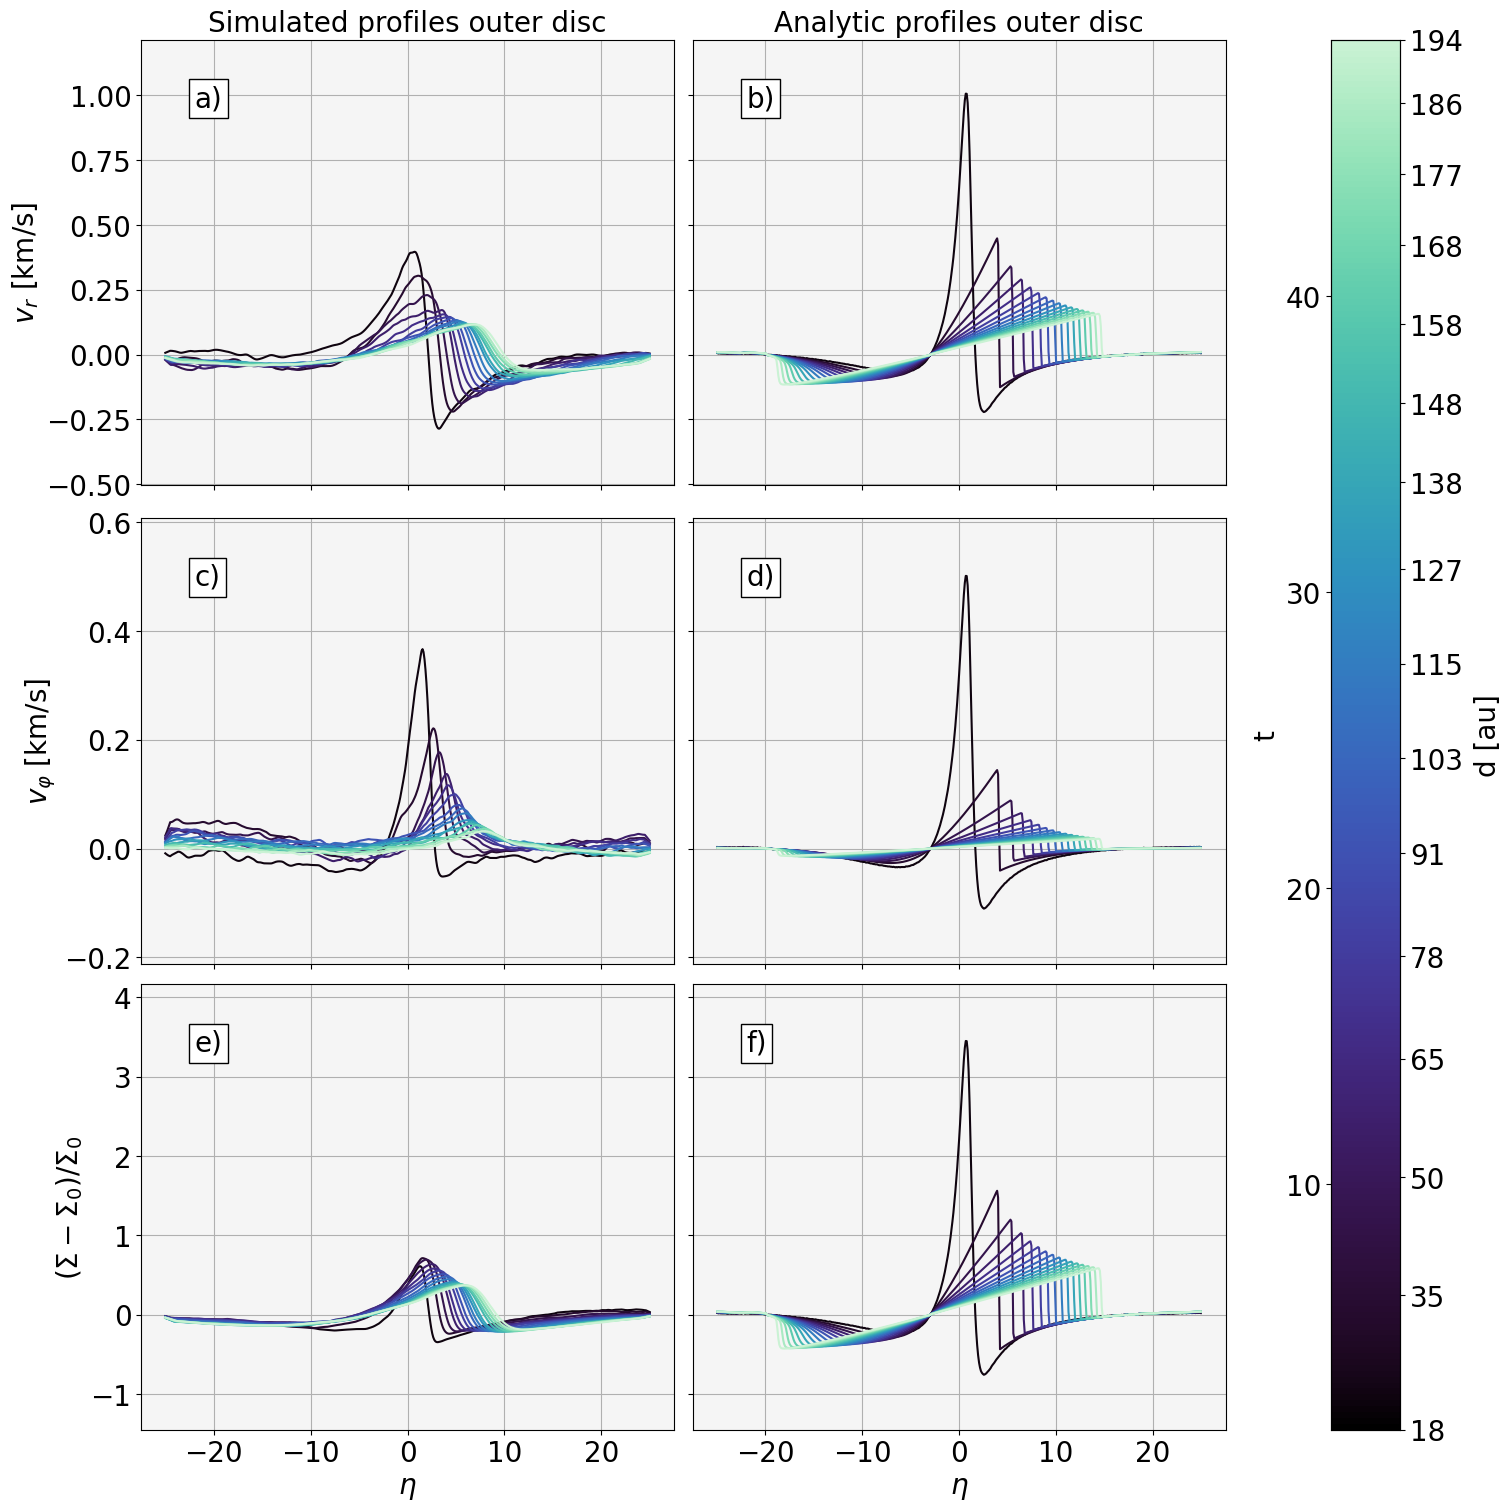
\includegraphics[width = 0.98\textwidth]{figures/comp_as_prof_out_high.png}
    \caption{Comparison between SPH (left) and semi-analytic (right) solutions for the perturbations induced by a $3.87 \, M_{\rm th}$ planet with orbital radius $r_{\rm p}=95.7 \, \mathrm{au}$. Wake profiles taken as slices of constant $t$, or equivalently $r$ are shown. The radial velocity, azimuthal velocity and density perturbations shown from top to bottom. The colourbar indicates the $t$ coordinate for each profile, as well as the physical distance $d$ from the planet location. Figure taken from \citeauthor{fasanoinprep.} (in prep.).}
    \label{fig:profile_comparison}
\end{figure}

However, moving away from the planet and deeper into the non-linear regime, the agreement between the analytical and simulated models improves.
Figure \ref{fig:profile_comparison} shows the outer wake profile as it evolves in $t$ for $3.87 \, M_{\rm th}$, compared between both models.
Remarkably, the accuracy in the non-linear regime seems to improve as $t$ increases.
The amplitude for each of the perturbations is in good agreement between the models after the wake was propagated only a few tens of $\mathrm{au}$ from the planet location.
The shocks produced by the inviscid Burger's equation evolution are however steeper than those found in the SPH model, like due to the artificial viscosity present in the simulation \citep{lodato2010}.
The wake profiles are more extended in $\eta$ in the analytics, but we do not seem to recover the over-damping found in the low mass regime by \citet{cimerman2021}.
The position of the outer shock in density, and so the shape of the wake, is also different between the models.
This is not surprising as the pitch angle of the spiral increases and deviates from the linear shape used in the analytics \ref{eq:phi_wake} for high mass planets \cite{zhu2015}.
It may be possible to calibrate for this increase in pitch angle from non-linear effects, see section 5.2 of \citet{cimerman2021} for more details.

The apparent accuracy of the solution in the semi-analytical model far from the planet in the high mass case is perhaps not surprising when considered in the context of the existence of the asymptotic solution given in section \ref{sec:asymptotic_N_wave}.
The more massive planets result in faster shock formation in the Burger's equation evolution, and so it makes at least qualitative sense that the asymptotic solution may also become valid earlier.
The agreement between the analytics and simulations for $t \gtrsim 10$ may therefore reflect that the solution quickly becomes independent of the initial condition, and that the asymptotic scaling in $\chi$ holds well for high planets resulting in the correct non-linear behaviour at some distance from the planet.
We defer further discussions of accuracy, including a full parameter study and a preliminary calibration of the semi-analytic method, to \citeauthor{fasanoinprep.} (in prep.).

\subsection{Velocity Perturbations} \label{sec:velocity_perts}

Following the method of \citet{bollati2021} to calculate the velocity perturbations in the non-linear regime results in a discontinuous solution at the edge of the linear box. 
The calculated amplitude of the velocity perturbations for $t>t_0$ is significantly less than that at the start of the non-linear solution where $t-t_0$ is small\footnote{Recall that $t_0$ is the $t$ coordinate at the transition between the linear and non-linear regimes.} (\citeauthor{fasanoinprep.}, in prep).
To investigate this discontinuity in velocity amplitude we re-derived the mapping from $\chi$ to $u$ and $v$ from \citet{rafikov2002a} and \citet{bollati2021}.
As we saw in section \ref{sec:nonlinear_evolution} the conservation of the Riemann invariant $R_+$ gives for the radial velocity perturbation
\begin{align}
    u = 2\frac{c_0-c}{\gamma - 1}=-2\frac{c_0}{\gamma + 1} \psi, \label{eq:u_rafikov}
\end{align}
where we define $\psi$ as
\begin{align}
    \psi = \frac{\gamma+1}{\gamma-1} \frac{c - c_0}{c_0},
\end{align}
which is the sound speed perturbation with a constant scale factor. Following \citet{rafikov2002a}, we then derive an expression for $\psi$ in terms of the density perturbation $\chi$ by assuming that the gas obeys a locally polytropic equation of state given by 
\begin{align}
    P = P_0(r) \left[ \frac{\Sigma}{\Sigma_0(r)} \right]^\gamma. \label{eq:poly_EOS}
\end{align}
The sound speed is then
\begin{align}
    c^2 = \frac{\partial P}{\partial \Sigma} = c_0^2(r) \left[ \frac{\Sigma}{\Sigma_0(r)} \right]^{\gamma-1}.
\end{align}
Rafikov then finds a relation between the density and sound speed perturbations, to second order in $\psi$, by expanding the above expression. 
This yields
\begin{align}
    \frac{\Sigma - \Sigma_0}{\Sigma_0} = \frac{2}{\gamma + 1}\psi + \frac{3 - \gamma}{\left( \gamma + 1  \right)^2} \psi^2 + \mathcal{O}(\psi^3). \label{eq:psi_exp}
\end{align}
Taking this expression to first order only, we write $u$ in terms of the density perturbation, and then in terms of $\chi$ by substituting equation \ref{eq:chi}. 
\begin{align}
    u = - c_0 \frac{\Sigma - \Sigma_0}{\Sigma_0} = -2 \frac{c_0}{\gamma + 1} \frac{\chi}{g(r)}. \label{eq:ap_rad_vel}
\end{align}
Similarly, \citet{rafikov2002a} finds the azimuthal velocity as
\begin{align}
    v \approx -2 \frac{c_0^2}{\Delta\Omega r} \frac{1}{\gamma + 1} \psi, \label{eq:v_rafikov}
\end{align}
giving to first order in $\psi$
\begin{align}
    v \approx - \frac{c_0^2}{\Delta \Omega r} \frac{\Sigma - \Sigma_0}{\Sigma_0} = - \frac{2}{\gamma + 1} \frac{c_0^2}{\Delta \Omega r} \frac{\chi}{g(r)}. \label{eq:ap_az_vel}
\end{align}
equations \ref{eq:ap_rad_vel} and \ref{eq:ap_az_vel} are the expressions used in \citet{bollati2021} to calculate the velocity perturbations in the non-linear regime. 
Since these are only accurate to first order in $\psi$, the assumption is made that $\psi \ll 1$, which is the weak shock approximation introduced in section \ref{sec:nonlinear_evolution}.
Since we are in particular interested in the velocity perturbations in the context of kinematics, and in planet masses comparable to the thermal mass, we should check if the assumption that $\psi \ll 1$ still holds for planets in the high mass regime.

We can derive an \textit{exact} expression for $\psi$ in terms of the density perturbation simply by rearranging equation \ref{eq:poly_EOS}. We find
\begin{align}
    \psi = \frac{\gamma + 1}{\gamma - 1} \left[ \left( \frac{\Sigma-\Sigma_0}{\Sigma_0} +1  \right)^{(\psi-1)/2}  -1 \right],
\end{align}
which can be written equivalently in terms of $\chi$ using equation \ref{eq:chi} giving
\begin{align}
    \psi = \frac{\gamma + 1}{\gamma - 1} \left[ \left( \frac{2}{\gamma + 1} \frac{\chi}{g(r)} +1  \right)^{(\psi-1)/2} -1 \right]. \label{eq:psi_exact}
\end{align}
We used equation \ref{eq:psi_exact} to check the aforementioned assumption that $\psi \ll 1$ in the non-linear regime solution. 
We constructed three \textsc{wakeflow} models using dimensionless units, with embedded planet masses of $0.5, 1.0$ and $2.0 \, M_{\rm{th}}$ respectively, all placed in orbit around a $1 \, M_{\rm{\odot}}$ star at an orbital radius of $r=1$. 
For all models, we chose $p=2.25$ and $q=0.25$ such that $\Sigma \propto r^{-1}$, and an aspect ratio $H/r=0.1$ at $r=1$. 
Figure \ref{fig:psi_comparison} shows the values of $\psi$ for each of these models, and demonstrates that even for the lowest planet mass model the value of $\psi$ nearby the planet is as large as $\sim \hspace{-0.23em} 0.6$ and so the second order terms will clearly be important even in this case. 
For masses $\ge \hspace{-0.23em} M_\mathrm{th}$ the problem is even worse, as there are regions where $\psi \gtrsim 1$ causing the expansion given in equation \ref{eq:psi_exp} to diverge.

\begin{figure}
    \centering
    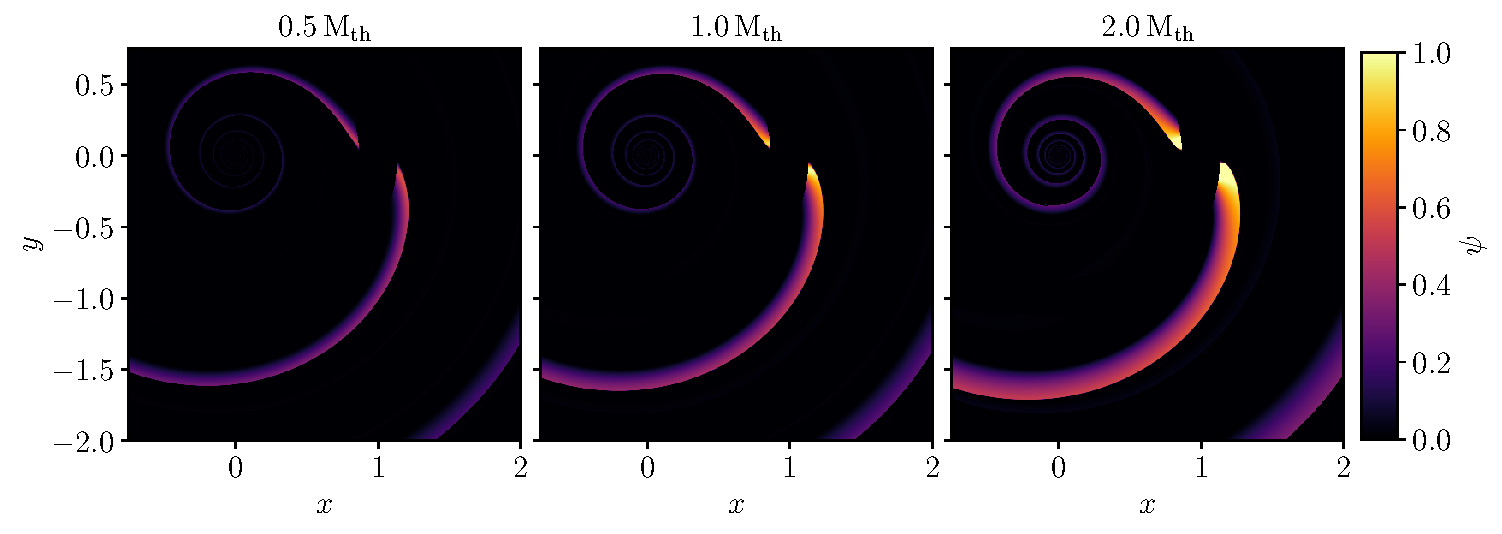
\includegraphics[width = 0.98\textwidth]{figures/psi 2.pdf}
    \caption{Comparison of the values of $\psi$ calculated from equation \ref{eq:psi_exact} for three \textsc{wakeflow} models with planet masses of $0.5, 1.0$ and $2.0 \, M_{\rm{th}}$ respectively. Clearly one cannot assume that $\psi \ll 1$ even for the lowest mass model, especially nearby the planet. For the two larger masses, there are even regions where $\psi > 1$.}
    \label{fig:psi_comparison}
\end{figure}

The choice of taking \ref{eq:psi_exp} to first order is justified in \citet{bollati2021} by noting that terms proportional to $\psi^2$ are discarded in the derivation of the Burgers evolution \ref{eq:burgers}, and thus also in the calculation of $\chi$ from which $u$ and $v$ are calculated.
The $u$ and $v$ calculated by their method are thus those that are consistent with the solution to Burger's equation \ref{eq:burgers}. 
However it is not clear that this gives the most physically reasonable results.
The argument for the velocities follows by relating the sound speed perturbation to the density perturbation through the equation of state \ref{eq:poly_EOS}.
However it is not clear that truncating the equation of state for density perturbations calculation \textit{necessitates} that the same truncation must be performed to find physically realistic velocity perturbations.

In order to obtain velocity perturbations that more closely match hydrodynamical simulations, and to reduce the amplitude discontinuity over the box, we derived expressions for both $u$ and $v$ as functions of $\chi$ without truncating the equation of state to first order in $\psi$. 
This is as simple as substituting equation \ref{eq:psi_exact} into equations \ref{eq:u_rafikov} and \ref{eq:v_rafikov}, yielding
\begin{align}
    u(\chi) &= -2 \frac{c_0}{\gamma - 1} \left[ \left( \frac{2}{\gamma + 1} \frac{\chi}{g(r)} +1  \right)^{(\psi-1)/2} -1 \right] \label{eq:u_chi_new} \\
    v(\chi) &\approx \frac{c_0}{\Delta\Omega r} u (\chi). \label{eq:v_chi_new} 
\end{align}
\begin{figure}
    \centering
    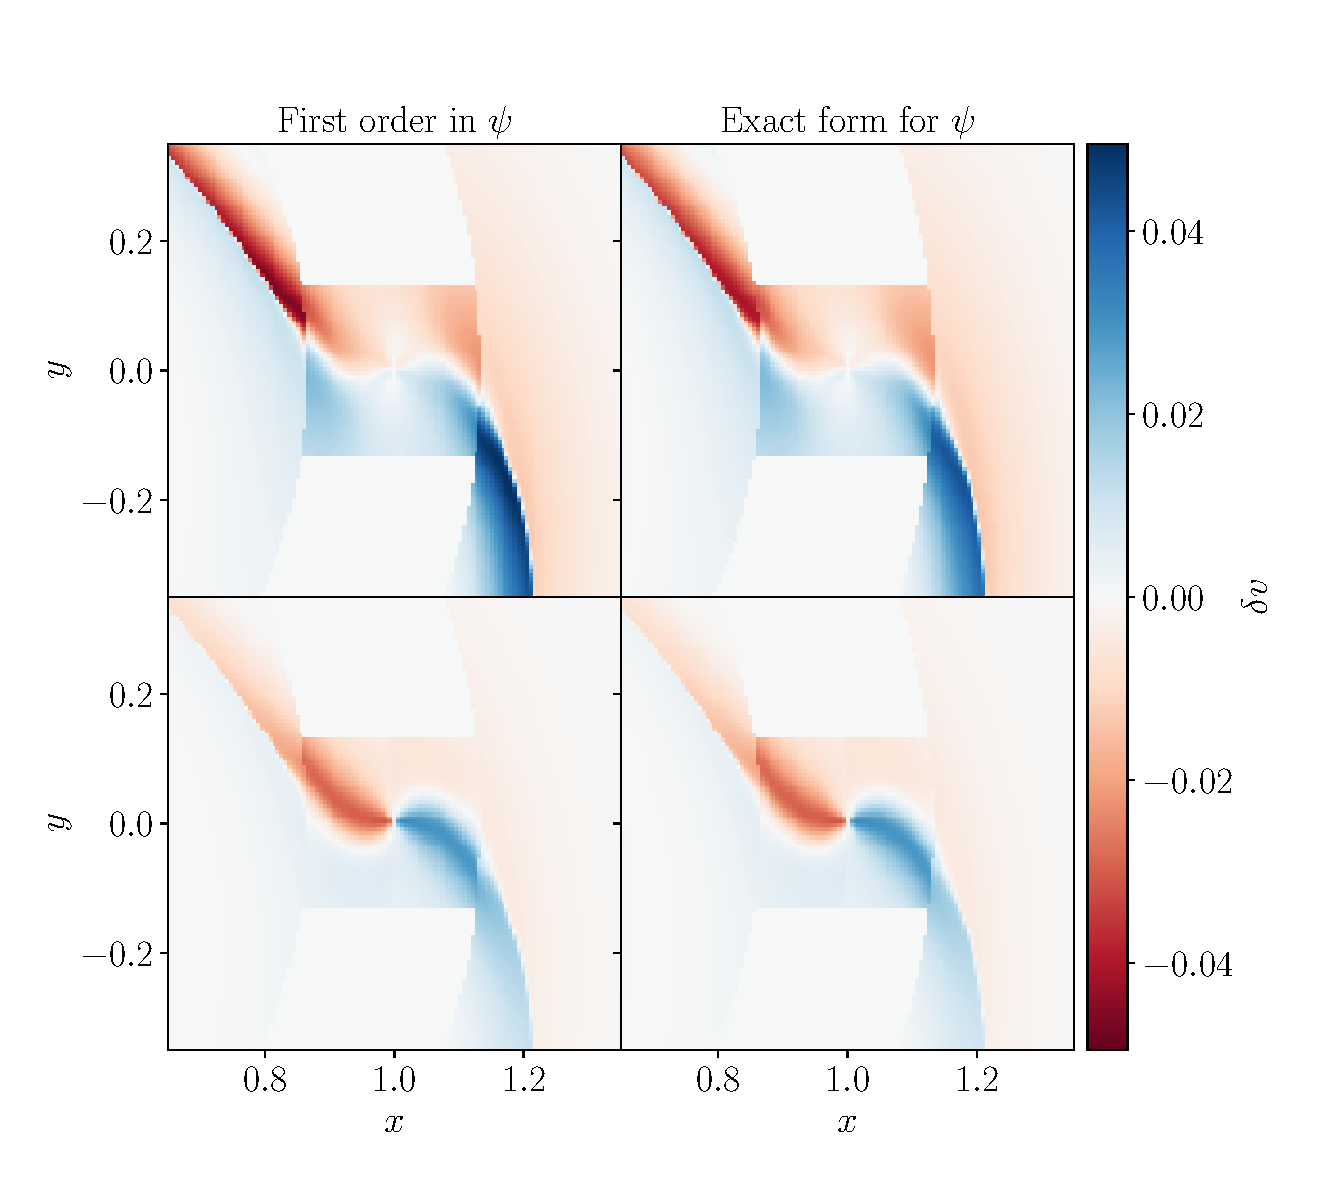
\includegraphics[width = 0.7\textwidth]{figures/0_5_mth.pdf}
    \caption{Comparison of the velocity perturbations calculated in the non-linear regime between the method of \citet{bollati2021} which is first order accurate in $\psi$ (left), and by using equations \ref{eq:u_chi_new} and \ref{eq:v_chi_new} which use the exact form for $\psi$ (right). The dimensionless radial velocity and azimuthal velocities are shown in the top and bottom panels respectively. The planet mass used in the model is $0.5 \, M_{\rm th}$. We see that the amplitude discontinuity is improved somewhat for the radial velocities, and basically unaffected for the azimuthal velocities.}
    \label{fig:0_5mth}
\end{figure}
\begin{figure}
    \centering
    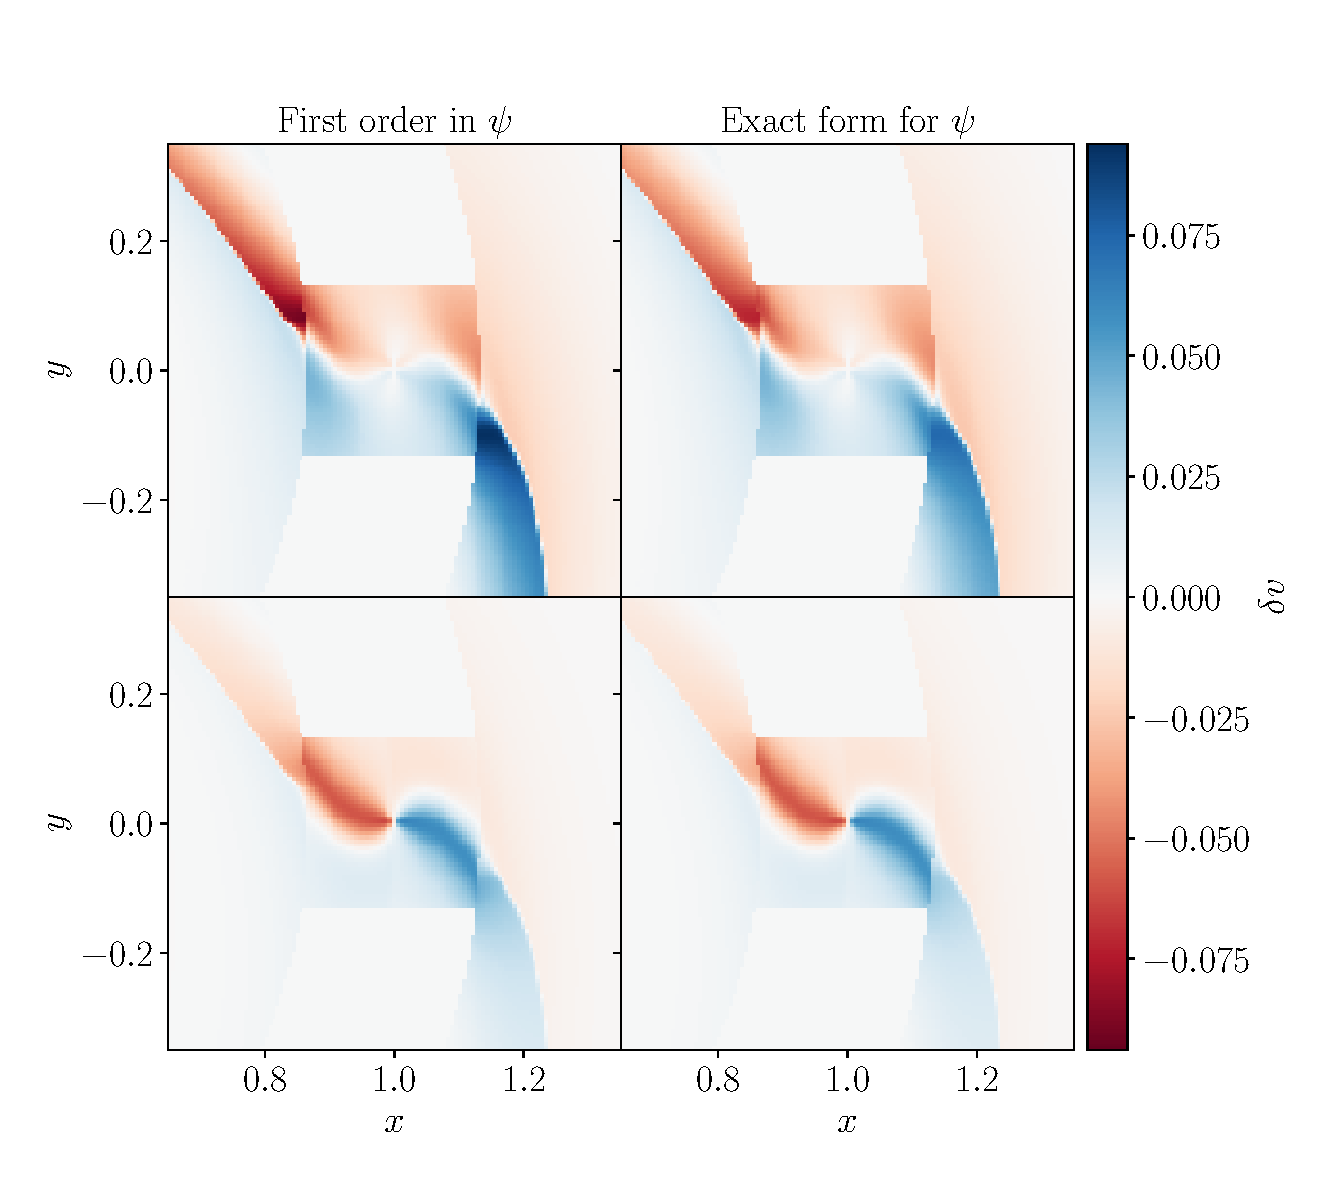
\includegraphics[width = 0.7\textwidth]{figures/1_0_mth.pdf}
    \caption{As in Figure \ref{fig:0_5mth}, except for a planet mass of $1.0 \, M_{\rm th}$. We see that the amplitude discontinuity is significantly improved for the radial velocities, but not for the azimuthal velocities.}
    \label{fig:1_0mth}
\end{figure}
\begin{figure}
    \centering
    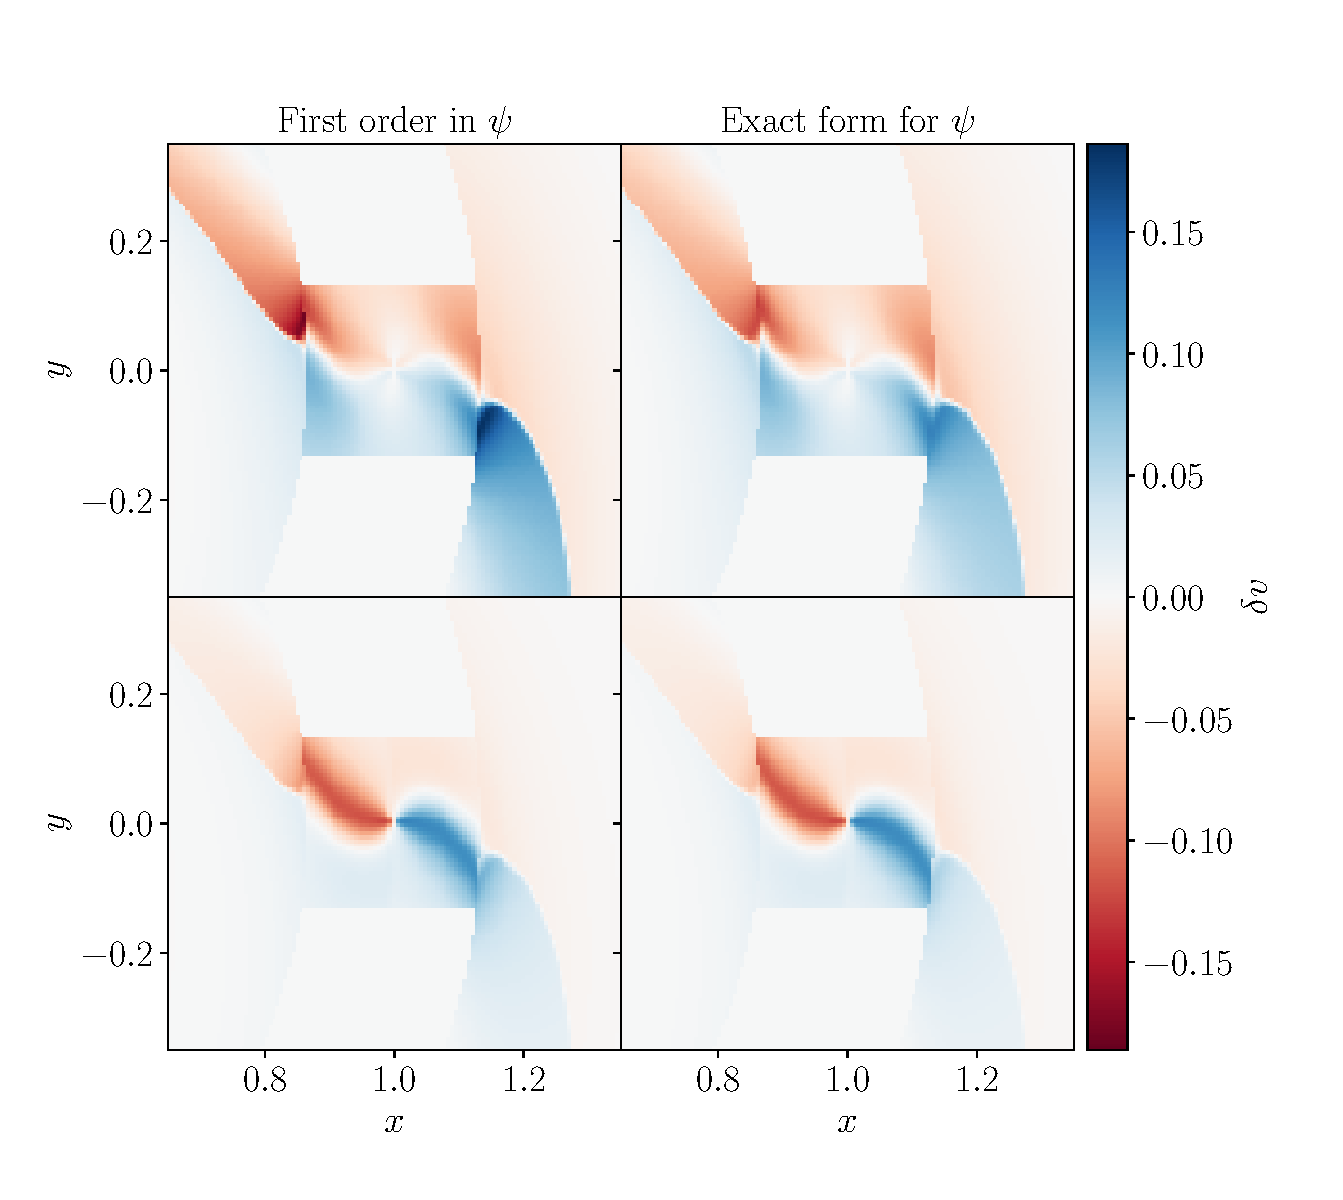
\includegraphics[width = 0.7\textwidth]{figures/2_0_mth.pdf}
    \caption{As in Figure \ref{fig:2_0mth}, except for a planet mass of $2.0 \, M_{\rm th}$. We see that the amplitude discontinuity is again significantly improved for the radial velocities, while unaffected or even slightly worse for the azimuthal velocities.}
    \label{fig:2_0mth}
\end{figure}
Figures \ref{fig:0_5mth}, \ref{fig:1_0mth} and \ref{fig:2_0mth} show a comparison of the velocities calculated from the above with those calculated to first order in $\psi$, for planet masses of $0.5, 1.0$ and $2.0 \, M_{\rm th}$ respectively. 
These are the same models as those used to create Figure \ref{fig:psi_comparison}. 
The plots are centred on the planet location, and they show that even for the lowest mass case the amplitude discontinuity is improved significantly for the radial perturbations by the new extraction using equation \ref{eq:u_chi_new}. 
This affect is increasingly significant for the more massive planets as can been seen in the $1.0$ and $2.0 \, M_{\rm th}$ cases. The azimuthal velocity case is however minimally affected. 
It is unclear why the radial perturbation is improved while the azimuthal perturbation is not.
However the derivation for $u(\psi)$ in \citet{rafikov2002a} comes from the conservation of the Riemann invariant $R_+$, while $v(\psi)$ is found in terms of $u$ by taking equation \ref{eq:phi_xi_v} and the terms $u \partial_\phi v$ and $u v / (\Delta \Omega r)$.
We conjecture that these terms are also important for larger mass planets, and that they could be responsible for the lack of improvement in the $v$ mapping.

Due to the reduction in the amplitude discontinuity, equations \ref{eq:u_chi_new} and \ref{eq:v_chi_new} are used to calculate the velocity perturbations in the non-linear regime in \textsc{wakeflow}. 

\section{Implications --- Non-Localised Velocity Kinks}

\citet{bollati2021} used 2D semi-analytic models to predict the morphology of velocity kinks that arise in kinematic observations \citep{pinte2018a} due to the velocity perturbations associated with the wake.
Figure \ref{fig:2D_kinks} shows the ``mock'' velocity channels that they generated by rotating the velocity perturbations to the line of sight for a disk inclined at $30^\circ$ from the sky plane.
They recover the abrupt sign reversal in velocity across the planet location first suggested by \citet{casassus2019}, the so-called \textit{Doppler flip}.
They also found that velocity kinks arise due to the intersection of the planet wake and the velocity channels, and that these kinks are spread throughout the disk.
Since at the time kinks were thought to be localised nearby the planet \citep{pinte2018a,pinte2019,pinte2020}, Bollati suggested that viscous damping may suppress the amplitude of the wave as it travels through the disk.
As we will see in chapter \ref{ch:wake_mapping}, velocity kinks are in fact \textit{not} localised nearby the planet location.
High resolution kinematic observations allow for the mapping of the planet wake in the disk through spatially correlated kinks spread throughout the disk \citep{calcino2022,teague2022,verrios2022}

\begin{figure}%[H]
    \centering
    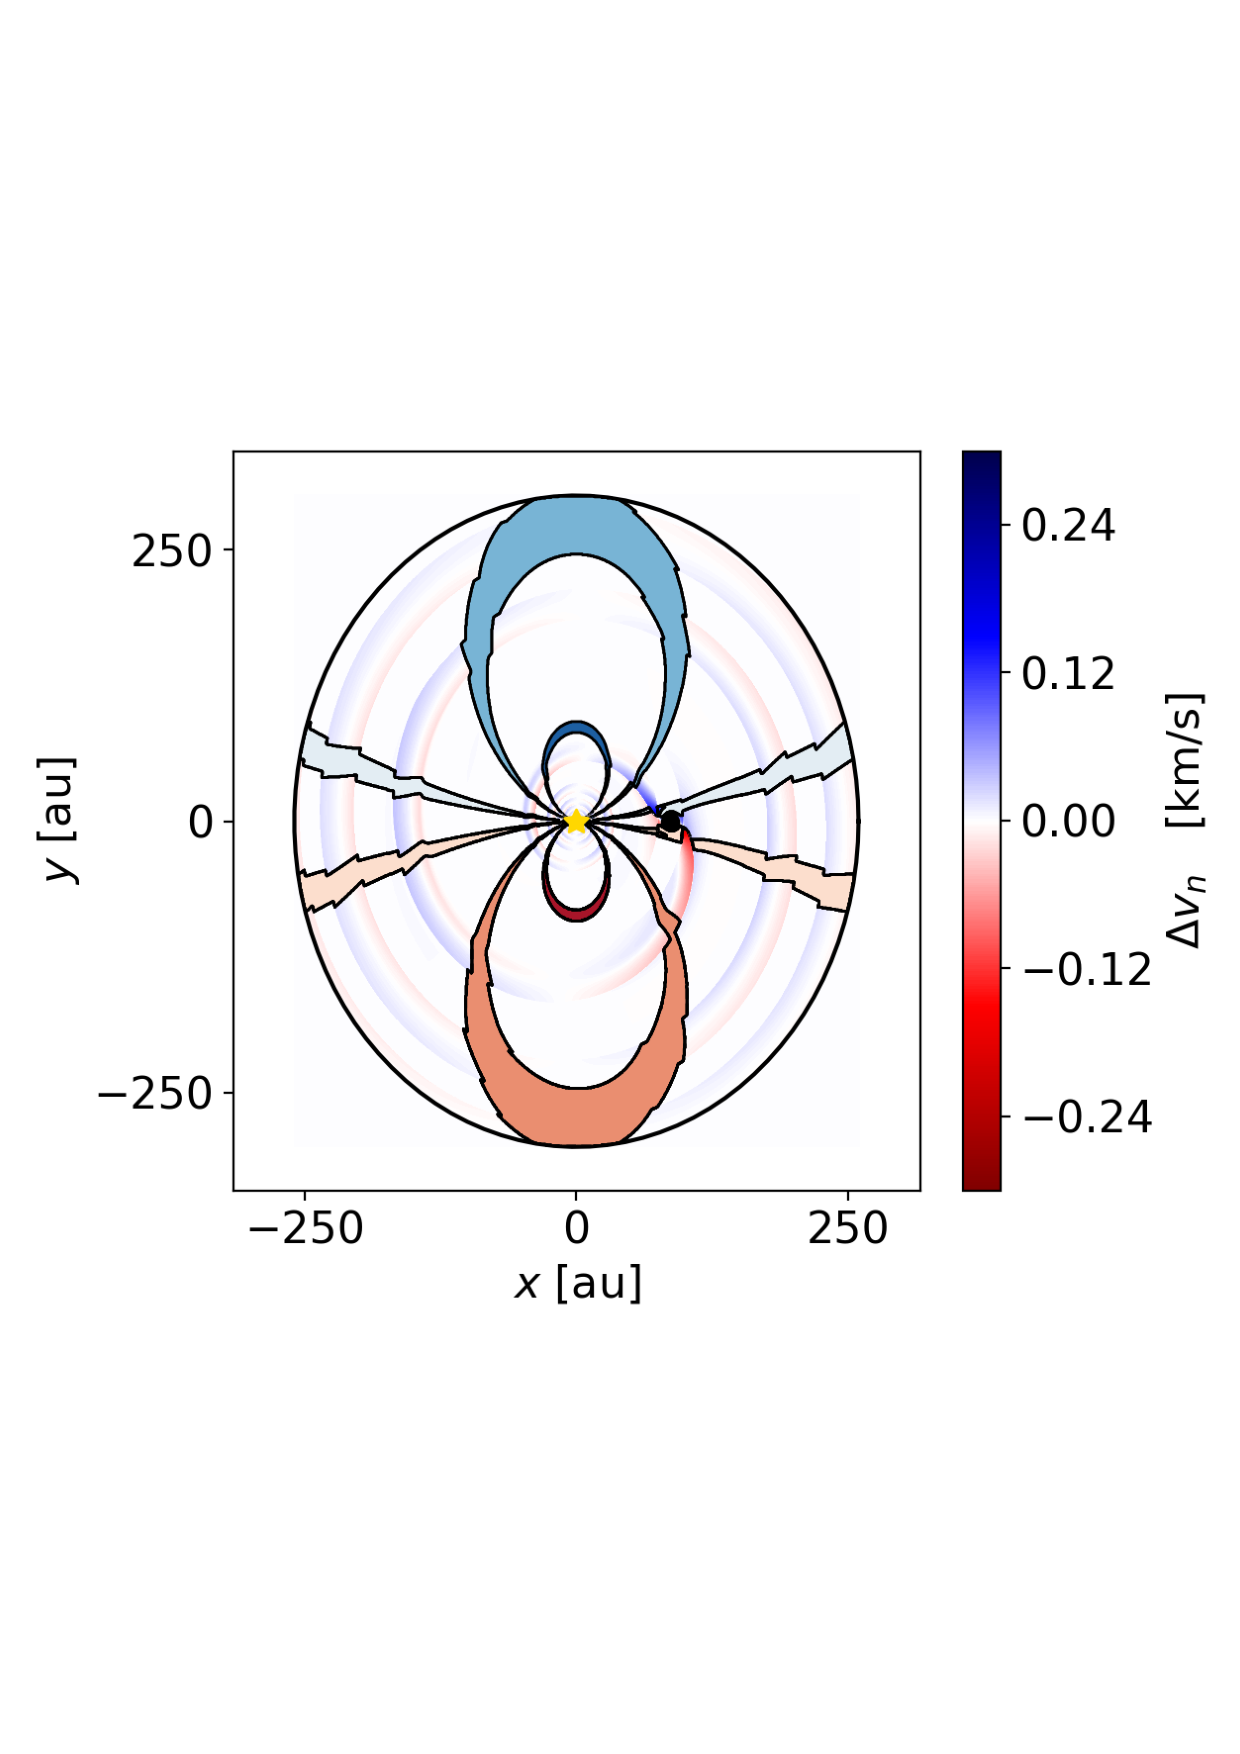
\includegraphics[width = 0.7\textwidth]{figures/bollati_2d_kinks.pdf}
    \caption{2 dimensional velocity channel maps generated from analytical models by \citet{bollati2021} for a disk inclined at $30^\circ$. The solid coloured bars represent velocity channels of width $\Delta v = 0.05 \, \mathrm{km/s}$, while the red and blue colouring gives the line-of-sight velocity perturbations. The planet and star locations are denoted by a black dot and yellow star symbol respectively. The chosen parameters for the model were $M_\star = 1\, M_\odot$, $M_{\rm p}=\mathrm{M_J}$, $r_{\rm p} = 100\, \mathrm{au}$ and $(H/r)_{\rm p}=0.1$.}
    \label{fig:2D_kinks}
\end{figure}

\section{Modelling the Kinematic Arc in HD~169142} \label{sec:hd169}

This section presents the semi-analytical modelling performed as a part of \citet{garg2022}, which is publicly available at \href{https://arxiv.org/abs/2207.02869}{\url{arXiv:2210.10248}}.

\subsection{Introduction}

HD~169142 is a disk-hosting Herbig Ae star located in the constellation of Sagittarius, at a distance of $117 \pm 4$ pc \citep{brown2016}.
The system's circumstellar disk appears almost face-on in the sky with an inclination of just $13^\circ$ \citep{raman2006,panic2008}.
The disk contains bright dust ring substructures at $\sim25$ au and $\sim65$ au, as well as a central cavity with radius $\sim22$ au.
These features have been observed through different tracers including scattered light \citep{quanz2013a,momose2015,pohl2017,bertrang2018} mid-infrared \citep{honda2012}, sub-millimetre with ALMA \citep{fedele2017,macias2019,perez2019} and centimetre with the Very Large Array \citep{osorio2014}.
The highest resolution of these studies showed that the outermost ring is actually three distinct rings separated by approximately $10$ au.
Various candidate point source detections have been made near the $r \approx 25$ au ring \citep{biller2014,reggiani2014,gratton2019}, but are disputed due to the possible confusion with disk material in their analyses \citep{ligi2018}.

This paper presents ALMA band 6 observations of the circumstellar disk around HD~169142.
We imaged the $^{12}$CO, $^{13}$CO and C$^{18}$O $J=2-1$ spectral lines at a resolution of $0.167 \, \mathrm{km/s}$, taking into account the Hanning Smoothing caused by the correlator.
The obtained angular resolutions of $0.07"$ and $0.1"$ allowed us resolve both density and kinematic substructures in the gas. Here, we will focus on the $^{12}$CO observations and on modelling the kinematics with the analytics.

\subsection{Observations and Analysis}

We imaged the $J=2-1$ line transitions of $^{12}$CO, $^{13}$CO and C$^{18}$O using ALMA band~6 observations from projects [2015.1.00490.S] and [2016.1.00344.S].
For details of the self-calibration and data reduction process, see \citet{garg2022}.

From equation \ref{eq:rot_eq_full}, the rotation velocity of the gas in a pressure-supported disk is given by 
\begin{align}
    \frac{v_{\rm gas}^2}{r} &= \frac{G M_\star r}{\left( r^2 + z^2  \right)^{3/2}} + \frac{1}{\rho_{\rm gas}} \partial_r P_{\rm gas}, \label{eq:gas_rotation}
\end{align}
where the first term is the typical Keplerian rotation and the second is the contribution by the radial pressure gradient.
As discussed in section \ref{sec:disk_rotation}, the second term typically results in sub-Keplerian motions.
To find kinematic substructures in the data, we wish remove the background motions of the disk associated with equation \ref{eq:gas_rotation} to isolate only the deviations from the bulk flow.
As a first step, we compute peak velocity $v_0$ maps by spectrally collapsing the data cube using the \textsc{Python} package \textsc{bettermoments} \citep{teague2018a}.
We chose specifically to use the \textit{Gaussian} method since it provides also the velocity error for each pixel $\delta v_0$ and has minimal statistical uncertainty \citep{yu2021}.

To obtain only the deviations from bulk rotation in $v_0$, we made use of the \textsc{Python} package \textsc{Eddy} \citep{teague2019}.
\textsc{Eddy} subtracts a best-fitting Keplerian rotation profile using a Markov Chain Monte Carlo (MCMC) method \citep{foreman-mackey2013}\footnote{The main point of using MCMC over a traditional optimisation methods is to obtain the uncertainties in the best fitting parameters by estimating the posterior distribution. However, we found that the error-bars we obtained were too small to be physically realistic, and so in appendix C of \citet{garg2022} we provide a parameter study around the best fit to investigate the true uncertainty.}.
We fit for the disk position angle (PA), central star mass $M_\star$, central star pixel location $(x_0,y_0)$ and systemic velocity $v_{\rm syst}$.
For the MCMC, we used 250 walkers and ran for 10,000 steps.
The data used in the fit were also restricted to within $1.5"$ from the centre of the image, as outside of this region was noise dominated.
The inner $0.2"$, equal to twice the beam width, was also exclude to avoid any bias resulting from beam smearing in the inner disk.
From fitting the $^{12}$CO data, we found best-fitting model parameters of $\mathrm{PA} = 5.33^\circ$, $M_\star = 1.47 \, \mathrm{M_\odot}$, and $v_{\rm syst} = 6.897 \, \mathrm{km/s}$.

To account for the pressure term of equation \ref{eq:gas_rotation}, we need the radial pressure gradient $\partial_r P_{\rm gas}(r)$.
Assuming an ideal gas equation of state, the pressure is given by 
\begin{align}
    P_{\rm gas}(r) = n_{\rm gas} k_{\rm B} T(r),
\end{align}
where $n_{\rm gas}$ is the gas number density, $k_{\rm B}$ is Boltzmann's constant and $T(r)$ is the temperature profile.
We calculated $n_{\rm gas}$ and $T(r)$ from the azimuthally averaged gas column density and brightness temperature profiles respectively, see \citet{garg2022} for further detail.

Finally, we made use of the best-fitting Keplerian rotation model, plus the radial pressure gradient, to subtract the bulk rotation from the peak velocity maps of the data to create kinematic residuals.
The result is shown in Figure \ref{fig:garg_arc}, along with the associated statistical significance.
We detect a kinematic excess of angular extent $\sim 105^\circ$ and magnitude $\sim 75 \, \mathrm{m/s}$ on the north side of the disk.
The excess is located between the $26$ au and $59$ au dust rings thus has a radial extent of approximately $30$ au.
The kinematic arc feature was however not detected in $^{13}$CO and C$^{18}$O, which may owe to the lower integration time of those observations, or may reflect that the rotation nearer to the mid-plane is less perturbed.

\begin{figure}
    \centering
    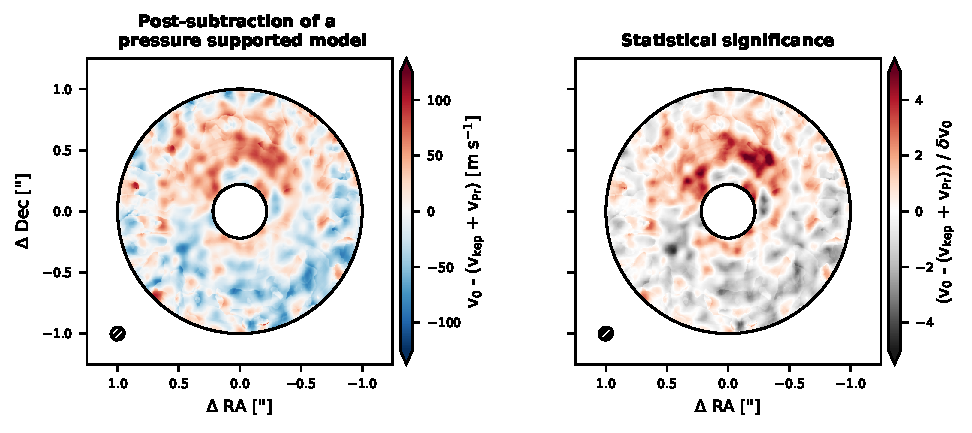
\includegraphics[width = 0.99\textwidth]{figures/garg_arc.pdf}
    \caption{Velocity residuals of the $^{12}$CO observations of HD~169142 calculated by the subtraction of a rotation profile including pressure support (left). Also shown is the residual velocities divided by the uncertainty in the peak velocity (right). The beam size is plotted in the bottom left corner of each panel, while the masked inner and outer regions are filled white \citep{garg2022}.}
    \label{fig:garg_arc}
\end{figure}

\subsection{Semi-Analytical Modelling} \label{sec:garg_analytics}

Notably, the feature we detected overlaps with the point source found in \citet{gratton2019} at a PA of $43.8^\circ$ and radial separation of $38$ au.
If the point source is a indeed a planet, perhaps the kinematic arc is associated with the velocity perturbations induced by the tidal forcing of the planet.
To test this scenario, we constructed semi-analytic models of the wake produced by a planet placed in the disk at the location of the \citet{gratton2019} point source using \textsc{wakeflow}.
We chose power law profiles for the unperturbed disk of $c \propto r^{-0.2}$ and $\Sigma \propto r^{-1}$, as well as an aspect ratio of $(H/r)_{\rm p}=0.08$.
The central star mass was chosen as $M_\star = 1.47 \, \mathrm{M_\odot}$ from the best-fitting model described in the previous section.
We used two $M_{\rm p}$ values of $1 \, \mathrm{M_J}$ and $10 \, \mathrm{M_J}$.

After the \textsc{wakeflow} models were calculated, we used the Monte Carlo radiation transfer code \textsc{mcfost} \citep{pinte2006,pinte2009} to generate synthetic $^{12}$CO $J=2-1$ observations.
The total gas mass of the model was set to $10^{-2} \, \mathrm{M_\odot}$ \citep{toci2019} and the gas-to-dust ratio was set to 100.
We use Mie theory \citep{mie1908} to calculate the optical properties of the dust grains, and assume that their size $a$ is distributed as $dn(a) \propto a^{-3.5} da$ where $n(a)$ is the number density of grains with size $a$.
The range of dust grain sizes used was between $0.03 \, \mathrm{\mu m}$ and $1$ mm, and they were taken to have a silicate composition \citep{weingartner2001}.
We assumed equal dust and gas temperatures, as well as local thermodynamic equilibrium.
The central star was modelled as an isotropically radiating blackbody, and $12.8\times 10^6$ packets were used to compute the dust temperature structure.
The relative CO abundance was taken to be $10^{-4}$, and the effects of CO freeze-out at $T < 20\, \mathrm{K}$, as well as photodissociation and photodesorption in regions of high UV were included \citep{pinte2018}.
The resultant channel maps had a channel spacing of $32 \, \mathrm{m/s}$, and the synthetic cubes were subsequently convolved spatially with a Gaussian of width $0.1"$ to replicate the beam size in the observations, as well as spectrally with a Hanning function of width $167 \, \mathrm{m/s}$ to replicate the effects of the correlator.

To create sky-plane velocity residuals, the cubes were collapsed spectrally in the same way as for the observations.
This whole process was then repeated except for models with no planet, and residuals were calculated as the different between the two velocity maps.
These residuals are presented in Figure \ref{fig:garg_analytics}.
Comparing these with Figure \ref{fig:garg_arc}, we see that in neither case do the analytic models recreate the arc found observationally.
The $1 \, \mathrm{M_J}$ planet model contains kinematic deviations that are far smaller than those observed.
On the other hand, the $10 \, \mathrm{M_J}$ produces residuals that while similar in amplitude, differ from the observations in shape, location and sign.
Of the two models, the $10 \, \mathrm{M_J}$ is more compatible with the observations but it still performs poorly.

Since the disk is nearly face-on, the observed kinematic structure may be dominated by vertical motions which are absent in the analytical models.
This may help to explain why the arc was absent in the $^{13}$CO and C$^{18}$O observations, since these trace the disk structure closer to the mid-plane.
For example, buoyancy spirals \citep{zhu2012,bae2021} excited by the planet in a thermally-stratified disk can result in significant vertical motions in the upper layers of the disk.
The planet wake in the mid-plane is expected to be dominated by radial motions \citep{rafikov2002a}, which would be hard to detect given the orientation of the disk.

A significant limitation to the analysis performed here is the accuracy of the \textsc{wakeflow} models nearby the planet.
Given the disk aspect ratio and central star mass, the thermal mass is only $\sim 0.5 \, \mathrm{M_J}$.
Thus the two models we have used here contain planets of masses $2 \, M_{\rm th}$ and $20 \, M_{\rm th}$.
In both of these cases the perturbations calculated close to the planet will be overestimated (\citeauthor{fasanoinprep.}, in prep.).
Unfortunately, in this case that is the region we are specifically interested in.
It is therefore only reasonable to interpret these results as upper bounds on the size of the perturbations that may be induced by the planet mass in each model.
We thus conclude that to explain the kinematic excess we have detected in the disk through our model requires a embedded planet of no more than $10 \, \mathrm{M_J}$.
%Planet masses were chosen based off the depth of the gas gap observed at $r=38$ au.
%Equation \ref{eq:kanagawa_gap_depth} relates the gap depth $\Sigma_{\rm p} / \Sigma_0$ to the aspect ratio $(H/r)_{\rm p}$, effective viscosity $\alpha$ and planet mass $M_{\rm p} / M_\star$.
%Taking our measured value of $\Sigma_{\rm p} / \Sigma_0 \approx 0.13$ in combination with  
%$(H/r)_{\rm p}=0.08$, and $\alpha=10^{-3}$ \citep{mulders2012,ansdell2018} gives an approximate planet mass of $\sim$
\begin{figure}
    \centering
    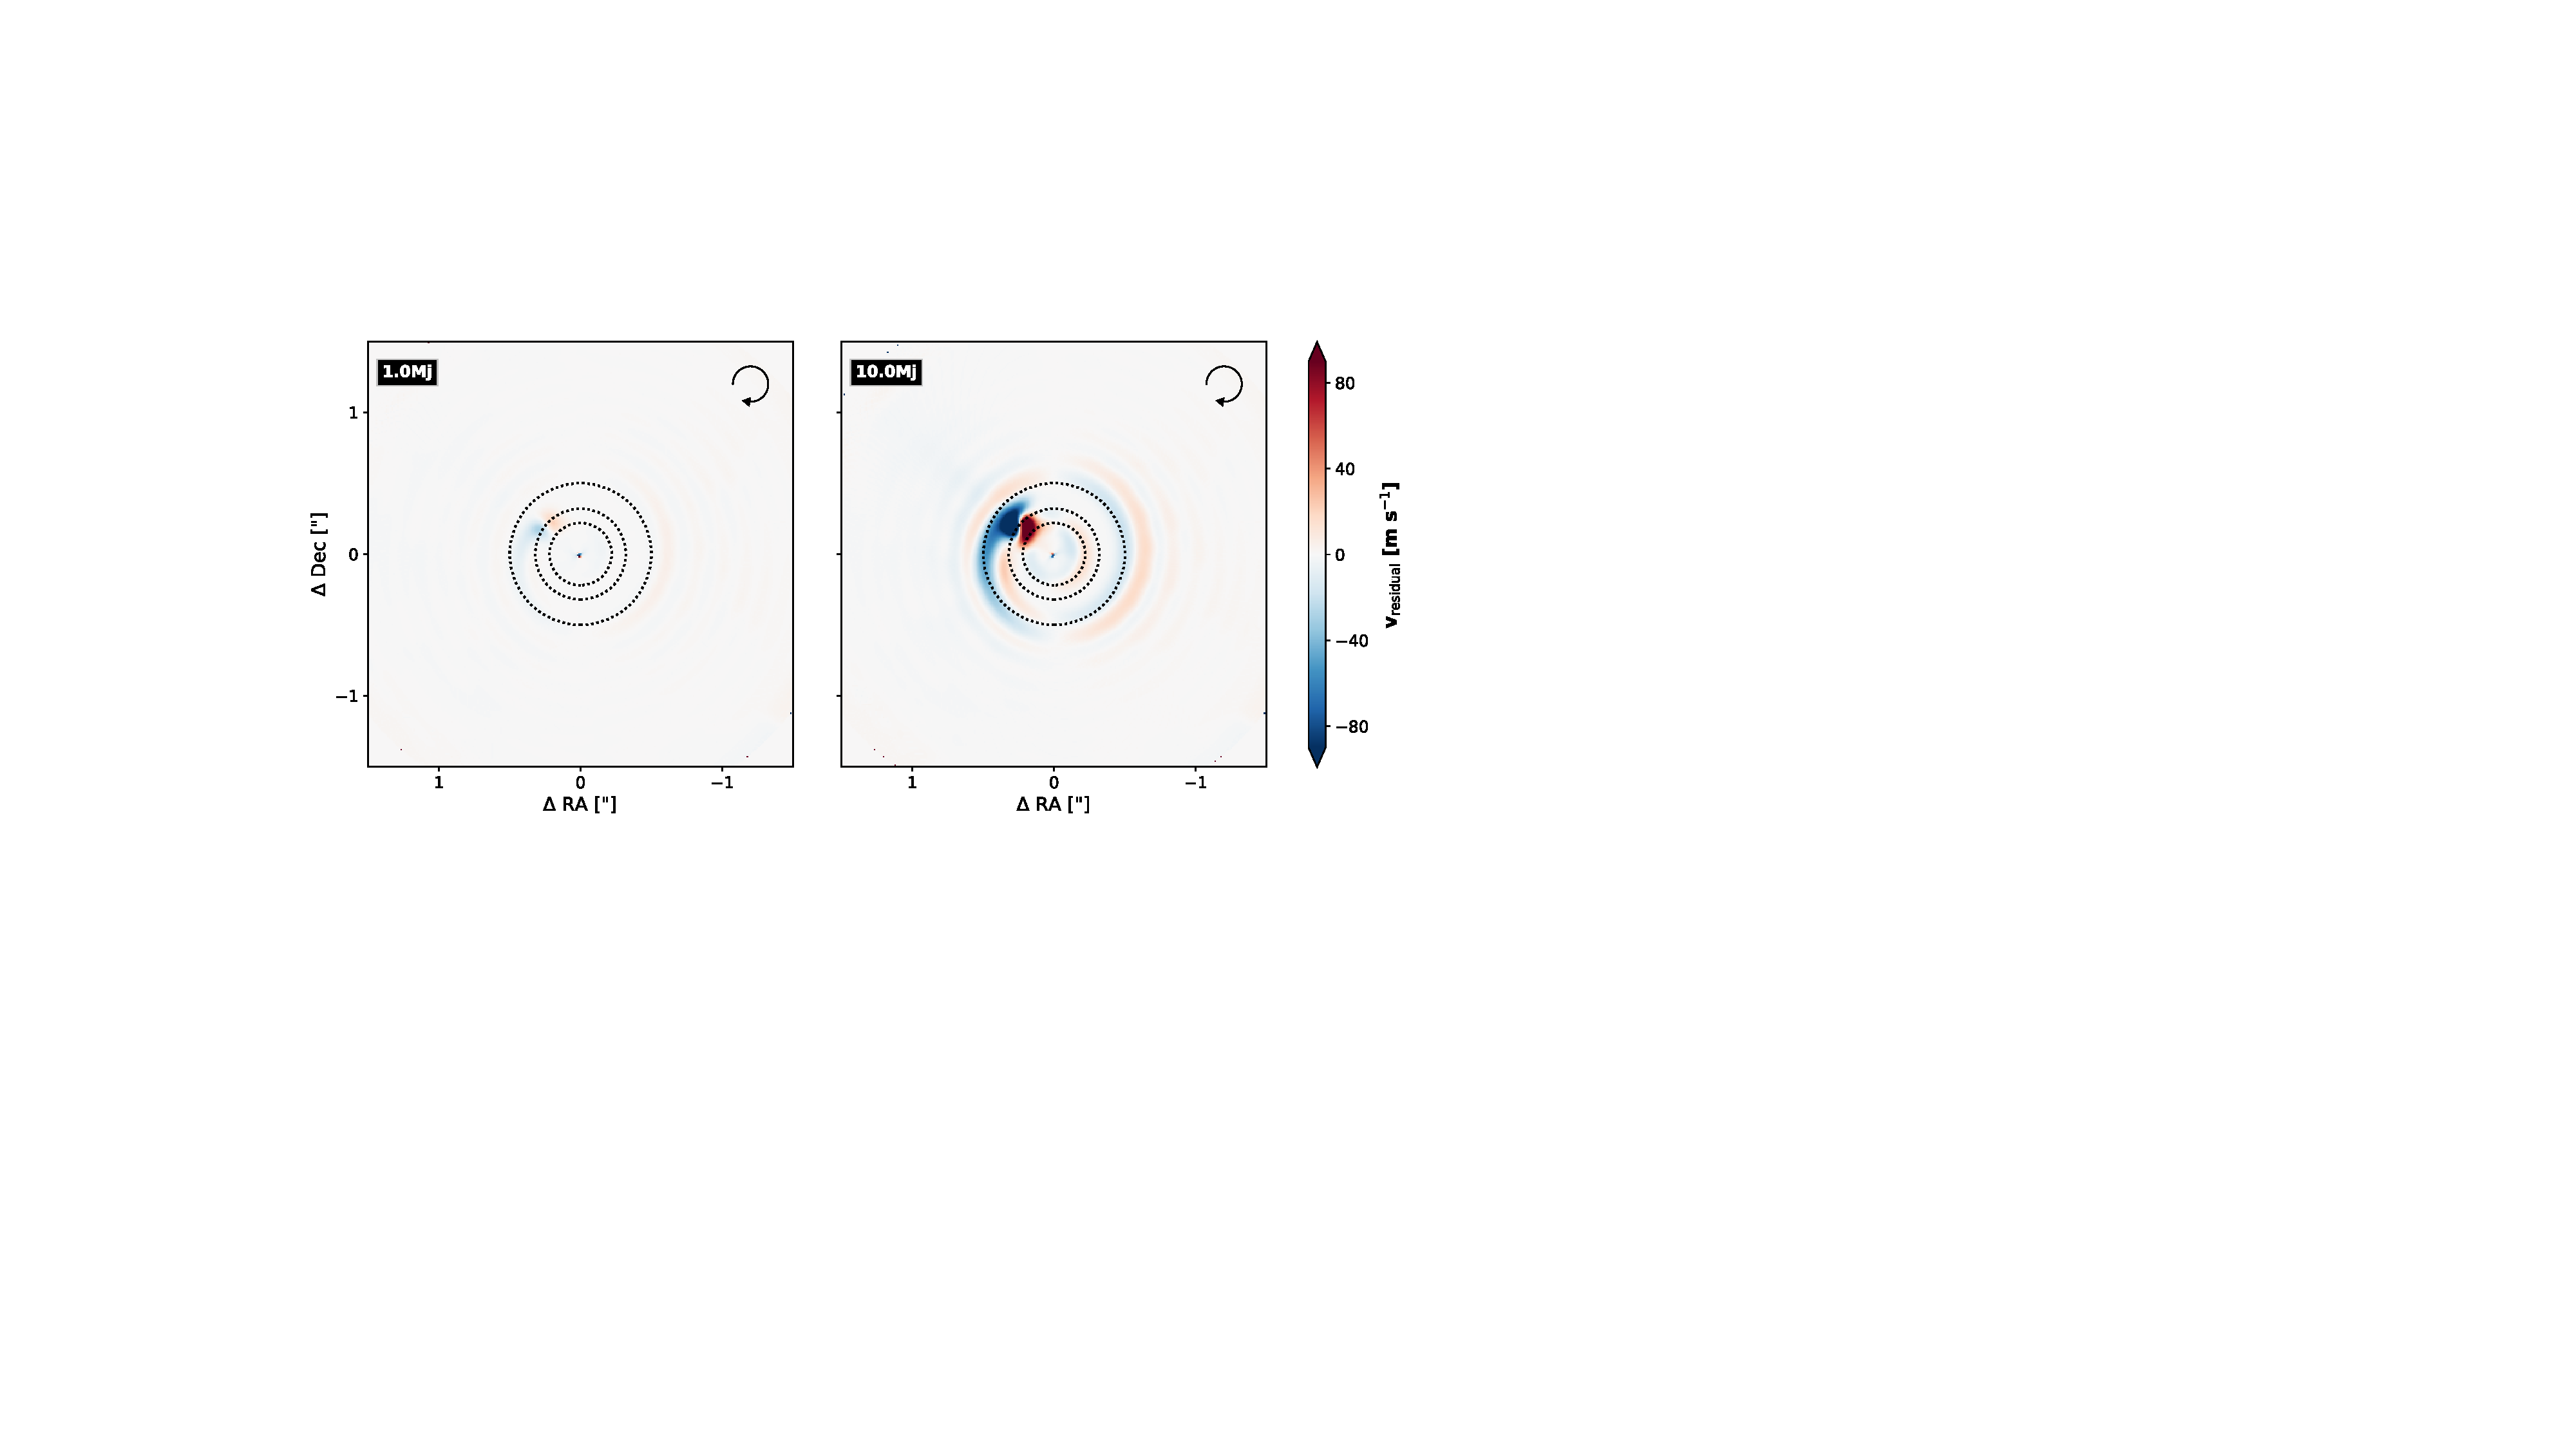
\includegraphics[width = 0.95\textwidth]{figures/garg_analytics_cw.pdf}
    \caption{Velocity perturbations from bulk rotation resulting from the tidal forcing of an embedded planet, calculated using \textsc{wakeflow} and \textsc{mcfost}. The $1 \, \mathrm{M_J}$ planet mass model is shown on the left, while the $10 \, \mathrm{M_J}$ model is shown on the right. The rotation direction of the disk is shown in the top-right of each panel \citep{garg2022}.}
    \label{fig:garg_analytics}
\end{figure}

    \chapter{Mapping the Wake in HD 163296 with Kinematics}
    
\section{Secondary Kinks}

\section{HD 163296} \label{sec:HD163wake}

\section{IM Lupi} \label{sec:IMLupiwake}

    \chapter{Planet Mass Recovery with Bayesian Inference}
    The final section of the thesis is concerned with trying to constrain the mass of protoplanets embedded in disks by quantitatively extracting the planet wake from kinematic observations.
We will build on the work presented in \citet{calcino2022}, where we showed that one can trace the shape of the planet wake, and amplitude of velocity kinks, through the peak velocity map.
In Section~\ref{sec:v0_fitting} we attempt to create a planet mass fitting procedure using synthetic peak velocity maps generated by projecting \textsc{wakeflow} models to the emitting surface of the disk.
Additionally, in Section~\ref{sec:mirror_residuals}, we present a method for locating the wake such as that in \citet{calcino2022}, but that does not rely on identifying patterns by eye.
%Finally in Section~\ref{sec:isovelocity_transform}, we demonstrate a potential method for extracting the wake information from observations that is model-independent.

\section{Peak velocity fitting} \label{sec:v0_fitting}

As shown in \citet{calcino2022}, the planet wake manifests in the peak velocity ($v_0$) map generated from molecular line emission observations as spatially correlated deviations from the expected smooth iso-velocity contour.
We additionally created synthetic $v_0$ maps by projecting semi-analytic models of the planet wake plus background rotation (Equation~\ref{eq:rot_eq_full}) to a the emitting layer of the disk, and then calculating the line-of-sight velocities in the disk.
Here, we will take the same approach to generating $v_0$ maps, but we will fit them onto the observed peak velocities.
The advantage of fitting in this way instead of first subtracting a best-fitting model for the background rotation and fitting to the residuals is two-fold.
First, creating residuals in this way is known to easily confuse the sign of the perturbations due to the high sensitivity to the background model (see the Appendix of \citealt{calcino2022}).
Secondly, fitting simultaneously for the background instead of assuming it allows for the determination of the covariances in the uncertainties between the background and planet perturbation models.
The best-fitting parameters for the planet mass and location will therefore not be conditioned on some background model, and we will be able to see any potential degeneracies between the parameters of each model.

\subsection{Models}

To generate our models, we first calculate the height of the emitting layer in the disk using the parameterisation \citep{pinte2018}
\begin{align}
    z(r) = z_0 \left( \frac{r}{r_{\rm ref}} \right)^\phi \exp \left( -\left[ \frac{r}{r_\mathrm{taper}} \right]^{\psi} \right), \label{eq:height}
\end{align}
which gives a flared structure with an exponential taper. $z_0$, $\phi$, $r_{\rm taper}$ and $\phi$ are then all model parameters that determine the height of the emitting layer. 
$r_{\rm ref}$ simply determines the radius at which the reference height $z_0$ and other parameters are defined, and we just set it to 100 au.
While this is a lot of freedom, the idea is to eventually use other methods of determining the height in this form such as the code \textsc{dynamite}\footnote{\url{https://github.com/cpinte/dynamite}} \citep{pinte2018} to determine best-fitting parameters, and then to place strong priors on the same parameters when fitting for the planet mass.

We then calculate the background velocity $v_{\phi,\mathrm{0}}$ for the disk at this emitting layer on a $300 \times 300$ Cartesian grid using
\begin{align}
    v_{\phi,\mathrm{0}}(r,z) = \sqrt{\frac{G M_\star}{r}} \left[ - \left(p + 2q\right) \left( \frac{H}{r} \right)^2 + \left( 1-2q \right) + \frac{2qr}{\sqrt{r^2 + z^2}}\right]^{1/2}, \label{eq:omega_wf_ps_full}
\end{align}
which is just Equation~\ref{eq:omega_wf_ps} rewritten as a velocity.
$p$ and $q$ determine the amount of pressure support in the disk, where $\rho \propto r^{-p}$ and $c \propto r^{-q}$ as usual.
$M_\star$ is the mass of the central star.
The scale height $H$ is calculated using
\begin{align}
    H(r) = H_{\rm ref} \left( \frac{r}{r_{\rm ref}} \right)^{\frac{3}{2} - q},
\end{align}
which comes from Equation~\ref{eq:scale_height}.
Thus $q$, $p$, $H_{\rm ref}$ and $M_\star$ are model parameters that determine the background rotation of the disk.

Next, the planet perturbations are calculated by calling \textsc{wakeflow} using the aforementioned parameters, as well as the planet mass $M_{\rm p}$ and orbital radius $r_{\rm p}.$
The calculated azimuthal velocity perturbations $v_{\phi,\mathrm{p}}$ and radial velocity perturbations $v_{r,\mathrm{p}}$ are then used with the background rotation $v_{\phi,\mathrm{p}}$ to calculate the total velocity components $v_r$ and $v_\phi$
\begin{align}
    v_r = v_{r,\mathrm{p}}, \qquad v_\phi = v_{\phi,\mathrm{0}} + v_{\phi,\mathrm{p}}.
\end{align}
These are then mapped to Cartesian components $v_x$ and $v_y$ so that we may use rotation matrices to obtain the line-of-sight velocities 
\begin{align}
    v_x &= -v_\phi \sin \phi + v_r \cos \phi, \\
    v_y &= +v_\phi \cos \phi + v_r \sin \phi.
\end{align}
Defining the velocity field in the frame of the disk $\mathbf{v} = (v_x, v_y, v_z)$ where we set $v_z=0$, we find that the velocity field projected to the sky plane $\mathbf{v'}=(v_x', v_y', v_z')$ is given by 
\begin{align}
    \mathbf{v'} =  R_z(p) R_x(i) R_z(\phi_{\rm p}) \, \mathbf{v}
\end{align}
where $R_x$ and $R_z$ are the standard Cartesian rotation matrices around the $x$ and $z$ axis respectively, $p$ is the position angle of the disk on the sky, $i$ is the inclination of the disk, and $\phi_{\rm p}$ is the azimuthal position of the disk as measured in plane of the disk.
The line-of-sight velocity is then simply given by the $v_z'$ component of the above.
Likewise, we can find the positions associated with the velocity field by rotating the position scalar field $\mathbf{x} = (x,y,z)$ in the same way to find $\mathbf{x'} = (x',y',z')$.
The sky coordinates $\Delta \, \mathrm{RA}$ and $\Delta \, \mathrm{Dec}$ in arcseconds for our projected line-of-sight velocity field is then simply
\begin{align}
    (\Delta \, \mathrm{RA}, \Delta \,\mathrm{Dec}) = \frac{1}{D} (x', y'),
\end{align}
where $D$ is the distance to the source in parsecs.

Figure~\ref{fig:model_v0} shows an example peak velocity map generated using this method for the disk of HD~163296, using the parameters from \citet{calcino2022} but with a planet mass of $1 \, \mathrm{M_J}$.

\begin{figure}
    \centering
    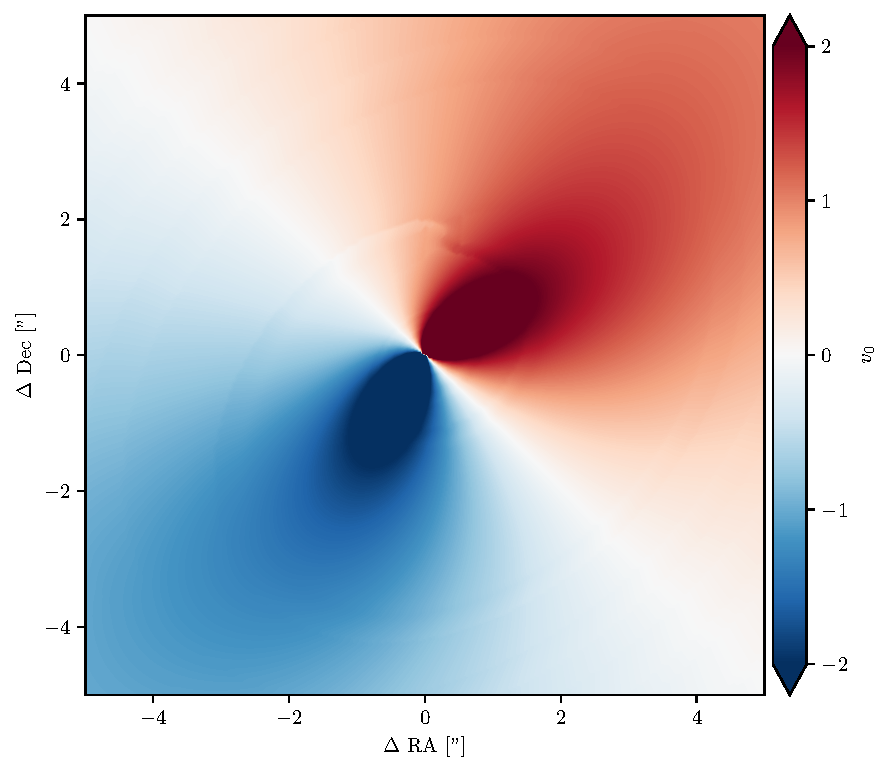
\includegraphics[width = 0.7\textwidth]{figures/thesis_contours_obs_model.pdf}
    \caption{Synthetic peak velocity map generated by projecting a semi-analytic model to the emitting layer. Parameters used in the model taken from \citet{calcino2022}, except for the planet mass which was set to $1 \, \mathrm{M_J}$. The planet wake is visible in the map due to the velocity perturbations it causes. The wake is most visible along near the semi-major axis as expected for radial-dominated motion \citep{rafikov2002a,bollati2021a,calcino2022}.}
    \label{fig:model_v0}
\end{figure}

\subsection{Fitting procedure}

Peak velocity maps produced from real kinematic observations are discretised in velocity at a resolution equal to the spacing of the channels\footnote{Unless using the higher order quadratic method mentioned in Section~\ref{sec:obs_analysis_garg}. Here we choose to use the usual peak velocity so that our uncertainties are related only to the beam size of the observations, and thus the positions of the iso-velocity contours. Using the quadratic method introduces statistical uncertainties in the velocities themselves.}.
We therefore discretise the velocity field from our models using the channel spacing.
Since the planet induces wiggles in the iso-velocity curves, we performed the fitting by minimising the distance between corresponding curves from the model and observations.
In a peak velocity map, we can find these curves simply through making a contour plot.
We therefore extracted the iso-velocity curves from both the observations and models by creating a contour plot with the \textsc{Python} package \textsc{Matplotlib}, which calculates the points along the contours using a marching squares algorithm \citep{hunter2007}.
Since peak velocity maps calculated from observations tend to be noisy, and often suffer from contamination by the lower surface of the disk, the calculated contours may be discontinuous towards the edge of the disk.
We therefore take only the longest continuous contour returned as representative of the iso-velocity curve for a specific velocity, and discard the others.
This can be seen in the left panel of Figure~\ref{fig:conts_obs_model}, which shows the peak velocity map from MAPS $^{12}$CO observations \citep{oberg2021} that we used in \citet{calcino2022}.
In the top left of the panel, we can see many small blobs due to backside contamination.
They grey lines show the contours that we extract, and the blobs are ignored.
The middle panel of Figure~~\ref{fig:conts_obs_model} shows the equivalent iso-velocity curves extracted from our example model in the previous section, this time without an embedded planet.
The right panel overlays the extracted model contours with the peak velocity map from the left panel.

\begin{figure}
    \centering
    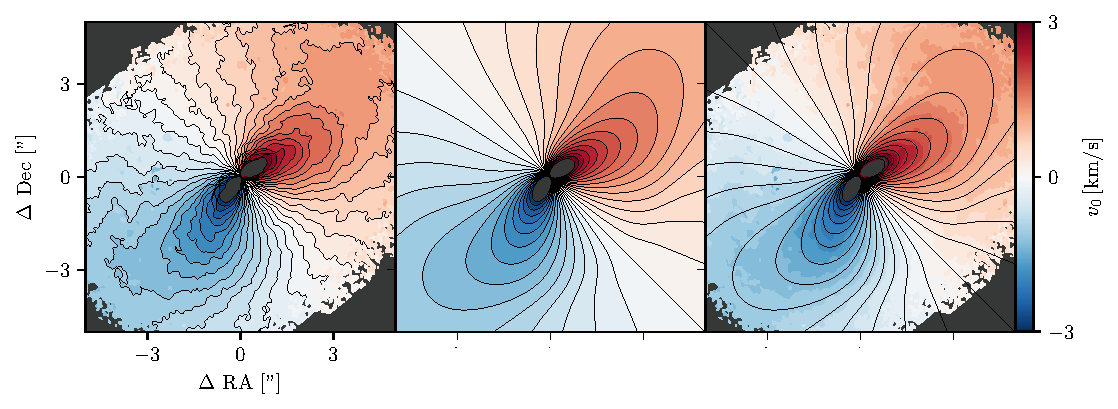
\includegraphics[width = 0.99\textwidth]{figures/thesis_plot_model_obs.pdf}
    \caption{The left panel shows a plot of the peak velocity map calculated from the $0.15"$ resolution $^{12}$CO line emission observations of the circumstellar disk of HD~163296 \citep{oberg2021}, with the contours extracted by our algorithm plotted in grey. The middle panel shows our model, with the extracted contours again plotted in grey. The right panel shows the contours extracted from the model plotted over the observed peak velocity.}
    \label{fig:conts_obs_model}
\end{figure}

In order to perform the fitting, we need some notion of distance between the lines of iso-velocity in the model and observations.
To do this, we summed the Euclidean distance between nearest points along each contour.
That is, for each point $(x_{\mathrm{o},j},y_{\mathrm{m},j})$ along for example the $\Delta v = 200 \, \mathrm{m/s}$ iso-velocity curve in the observations, we found the closest point $(x_{\mathrm{m},j},y_{\mathrm{m},j})$ on the $\Delta v = -200 \, \mathrm{m/s}$ iso-velocity curve in the model, and calculated the distance $d_j^2 = (x_{\mathrm{o},j} - x_{\mathrm{m},j})^2 + (y_{\mathrm{o},j} - y_{\mathrm{m},j})^2$.
Summing these distances then yields the total ``distance'' between the two curves $D = \sum_j d_j$.
This distance was calculated for all of the pairs of iso-velocity curves extracted.
The uncertainty in this distance is $\sigma_{\rm beam}$, which is the angular size of the telescope resolution.
We therefore chose our reduced chi squared to be
\begin{align}
    \chi_{\rm red}^2 = \left( \sum_i^{N_{\rm C}} N_i - N_{\rm p} \right)^{-1} \left( \sum_{i}^{N_{\rm C}} \sum_{j}^{N_i} \frac{(x_{\mathrm{o},ij} - x_{\mathrm{m},ij})^2 + (y_{\mathrm{o},ij} - y_{\mathrm{m},ij})^2}{\sigma_{\rm beam}^2} \right),
\end{align}
where the $i$ index sums over each iso-velocity contour of a particular line-of-sight velocity, and the $j$ index sums over all the points along that contour.
$N_i$ is therefore the number of points along observed contour $i$, while $N_{\rm C}$ is the total number of contours.
$N_{\rm p}$ is the number of parameters in the model.

\subsection{Background fitting}

Before attempting to fit for planet mass, we wanted to confirm that we could obtain $\chi^2$ minima in parameter space for sensible values of a model including only the unperturbed background disk.
To do this we used the JvM corrected \citep{jorsater1995} $^{12}$CO $J=2-1$ \textit{robust=0.5} line emission observations of HD~163296 from the MAPS large program (2018.1.01055.L, \citealt{oberg2021,czekala2021})\footnote{The data are available for download at \url{http://alma-maps.info/}.}, which has a channel spacing of $200 \mathrm{m/s}$, and a beam size of $0.15"$.
This is the same data we used in \citet{calcino2022}.
We also assumed a systemic velocity of $v_{\textrm{los}}= 5.76$ km/s \citep{teague2021} and a distance of $101.5 \, \mathrm{pc}$ \citep{gaiacollaboration2018}.

We then adopted the best-fitting background model parameters used in \citep{calcino2022}, and varied only parameter one at a time to see whether each found a minimum $\chi^2$ value.
The results of the grid search are shown in Figure~\ref{fig:grid_chisq_background}.
The top row of the figure shows the parameters that determine the background rotation.
We see that for the rotation parameters, both $M_\star$ and $H_{\rm ref}/r$ find minima around approximately $1.8 \, \mathrm{M_\star}$ and $0.11$ respectively. 
These both compatible with the expected values from the literature, differing by less than 5\% in each case \citep{pinte2018a}.
However the $p$ and $q$ indices are both constrained very poorly and neither find a minimum.
This is perhaps not surprising when considering that changing either of this has little effect on our model, as they merely change the background rotation very slightly as part of the pressure gradient term.
The aspect ratio $H/r$ is also only responsible for the pressure correction, but since it is squared in Equation~\ref{eq:omega_wf_ps_full} it has a larger effect.
It therefore seems unlikely that $p$, $q$ and $H/r$ could be disentangled from fitting purely our background model.
However, both $H/r$ and $q$ are both responsible for determining the shape of the wake once we add a planet (see Equation \ref{eq:power_law_wake}), which may allow us to constrain them more effectively.

\begin{figure}
    \centering
    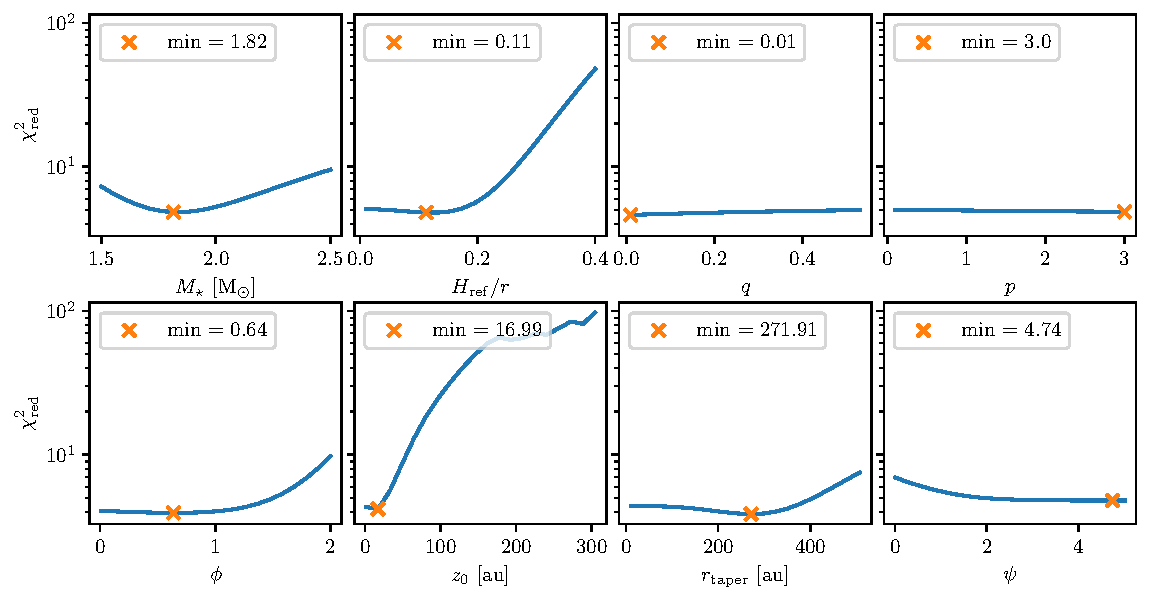
\includegraphics[width = 0.95\textwidth]{figures/chi_sq_background_hd163.pdf}
    \caption{$\chi_{\rm red}^2$ values fitting an unperturbed disk model to the MAPS $^{12}$CO peak velocity map of the HD~163296 disk, calculated by varying each parameter one at a time while keeping the others fixed. The top row is parameters tha determine the disk rotation, while the bottom row parameters determine the $^{12}$CO emission surface. The parameter values for the best-fit are marked by orange crosses. We see that the parameters that determine the pressure support $p$ and $q$, as well as the disk taper rate $\psi$, are poorly constrained.}
    \label{fig:grid_chisq_background}
\end{figure}

Turning our attention to the parameters that determine the emission surface, shown in the bottom row of Figure~\ref{fig:grid_chisq_background}, we see that all the parameters found a minimum.
These minima occur at values of $\phi = 0.64$, $z_0 = 16.99 \, \mathrm{au}$, $r_{\rm taper} = 271.91 \, \mathrm{au}$, and $\psi = 4.74$.
Comparing with the values found by \citet{law2021a}, which were $\phi = 1.851$, $z_0 = 39.37 \, \mathrm{au}$, $r_{\rm taper} = 239.74 \, \mathrm{au}$, and $\psi = 1.182$, we see that $\phi$, $z_0$ and $\psi$ are significantly different.
The difference in $\psi$ is not too surprising, as the rate of exponential taper of the height of the disk likely does not effect the model very much.
This is because the taper really only starts to have an effect at around $300$ au or $\sim3"$, which is near the edge of the data.
The cause of the difference in values were obtained for $\phi$ and $z_0$ is less clear.
They imply that the inner disk stays flatter for longer than found by \citet{law2021a}, before rising more steeply in the outer disk.
This may be due to our method of calculating $\chi^2$, which relies on Euclidean distances.
Changing the height in the inner disk does not result in much change to the iso-velocity contours, and so measuring the height in the inner disk in this way perhaps provides a poor constraint.
The results do seem to recover the height in the outer disk more accurately, since $r_{\rm taper}$ is relatively close to the \citet{law2021a} value.
Of course, all this comes with the important caveat that each minimum is conditioned on the other parameters being correct, since we are varying them one at a time here.

\subsection{Planet fitting}

Next, we performed the same analysis as above, except including the perturbations induced by a planet.
We used a $2.0 \, \mathrm{M_J}$ planet, placed at an orbital radius of $256$ au and a planet azimuth of $55$ degrees \citep{pinte2018a,calcino2022}.
The results for the background parameters are presented in Figure~\ref{fig:grid_chisq_planet_bg}, while the results for the planet parameters are shown in Figure~\ref{fig:grid_chisq_planet}.

For the background parameters shown in the top row, all of the minima are different to those found in Figure~\ref{fig:grid_chisq_background}, where a planet was not included. The central star mass has increased by $\sim10$\%, $H_{\rm ref}/r$ has halved, and $p$ and $q$ show different behaviours.
There are multiple possible explanations for this.
The first, and more straightforward, is that the kinks we have added to the model contours by including a planet allows for a better fit to background features.
Alternatively, it may be due to the effect those parameters have on the planet perturbations.
For example, reducing $H_{\rm ref}/r$ will significantly reduce the value of the thermal mass (see Equation~\ref{eq:thermalmass}).
This in turn increases the value of $M_{\rm p} / M_{\rm th}$, resulting in larger kink amplitudes.
$H_{\rm ref}/r$ and $q$ both determine the shape of the wake (see Equation~\ref{eq:power_law_wake}), which is likely to change how well the kinks fit the data.

For the emission surface parameters (bottom row of Figure~\ref{fig:grid_chisq_planet_bg}), we again find differences to the purely background fit.
$\phi$ and $z_0$ are both larger, which in each case increases the height of the emitting layer\footnote{More precisely, increasing $\phi$ makes the emitting layer more flared, whereas increases $z_0$ scales the height by a constant for all $r$.}.
The radius of the taper is $\sim 25$\% larger, which has the result fo increasing the height of the disk model in the region around $300$ au.
The result for $\psi$ is not much different, with a similar behaviour to in the background case where any large value of $\psi$ performs well.
These differences in height corroborate the idea that adding the planet kinks can result in a different best-fit for just the background as already mentioned.
These parameters do not have any effect of the shape of the wake or the amplitude of the kinks, unlike the parameters that determine the rotation.

\begin{figure}
    \centering
    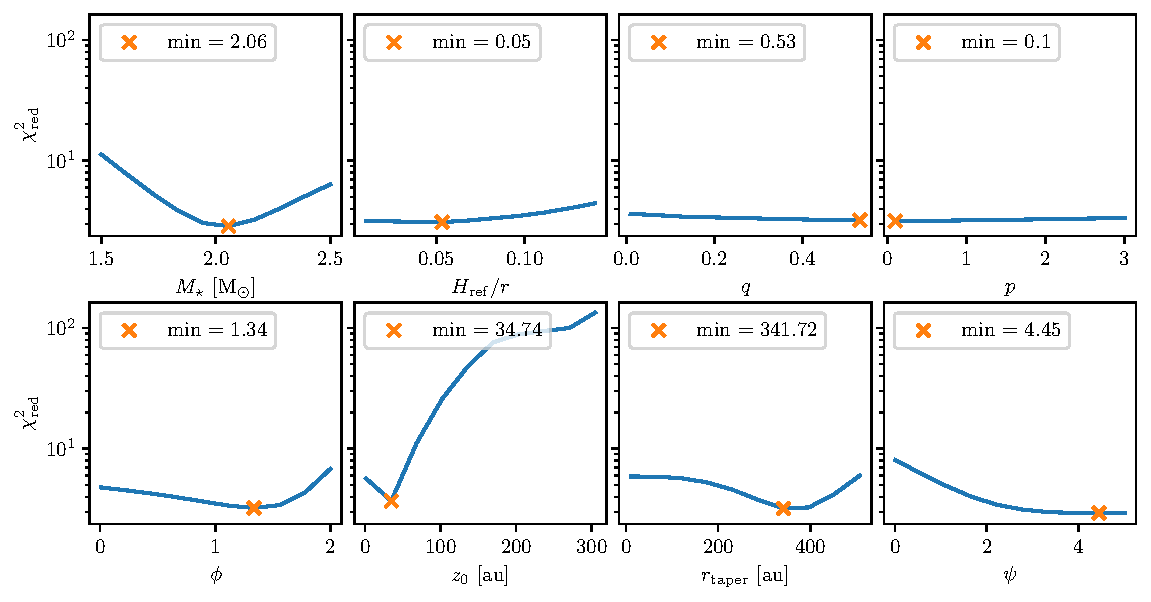
\includegraphics[width = 0.95\textwidth]{figures/chi_sq_background_planet_hd163.pdf}
    \caption{$\chi_{\rm red}^2$ values fitting an disk model with a $2 \, \mathrm{M_J}$ perturbing planet to the MAPS $^{12}$CO peak velocity map of the HD~163296 disk, calculated by varying each parameter one at a time while keeping the others fixed. The top row is parameters tha determine the disk rotation, while the bottom row parameters determine the $^{12}$CO emission surface. The parameter values for the best-fit are marked by orange crosses. The introduction of a planet results in different local minima for the background disk parameters.}
    \label{fig:grid_chisq_planet_bg}
\end{figure}

\begin{figure}
    \centering
    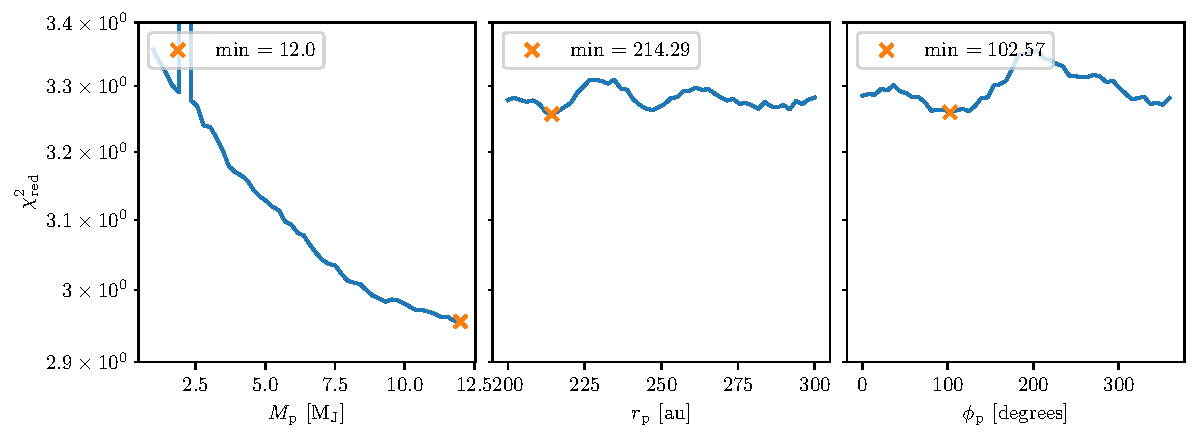
\includegraphics[width = 0.95\textwidth]{figures/chi_sq_planet_hd163.pdf}
    \caption{$\chi_{\rm red}^2$ values fitting an disk model with a $2 \, \mathrm{M_J}$ perturbing planet to the MAPS $^{12}$CO peak velocity map of the HD~163296 disk, calculated by varying each parameter one at a time while keeping the others fixed. The left panel shows the result of varying the planet mass, while the middle and right panels show the results for varying $r_{\rm p}$ and $\phi_{\rm p}$ respectively. The parameter values for the best-fit are marked by orange crosses.}
    \label{fig:grid_chisq_planet}
\end{figure}

Figure~\ref{fig:grid_chisq_planet} shows the results for the planet parameters themselves.
Looking first at the planet mass, we see that the best fitting mass is the largest in the interval that we tried, $12.5 \, \mathrm{M_J}$.
We did not allow for planets larger than this as the semi-analytic solution becomes very inaccurate and poorly behaved (see Section~\ref{sec:high_mass}).
This result is surprising, as it has previously been found that a planet of mass $3$--$4 \, \mathrm{M_J}$ accurately recreates the velocity kink induced nearby the planet.
Additionally, $r_{\rm}$ actually finds two minima, one at around $240$ au, which is close to what we would expect from \citet{calcino2022}.
The other minimum at $215$ is intriguing, as there have been claims of an additional planet closer to the star \citep{teague2018,pinte2020}.
It may be that this minimum results from the wake attempting to fit the arc feature mentioned in \citet{teague2021} and \citet{calcino2022} (see the opaque crosses in Figure~1 of the latter).
Finally, $\phi_{\rm p}$ finds a minimum at $\sim100$ degrees, which is significantly different to the $\phi_{\rm p}=55$ degrees that we used in \citet{calcino2022}.
Since tightly-wound spiral structure varies rapidly in $\phi$ as the radius changes slowly, it may be that this is because the value of $r_{\rm p}=256$ au we have chosen is not quite correct.

\subsection{Model-model fitting} \label{sec:model_model_fit}

It is not exactly clear how to interpret the results presented in the previous section.
While minima were found for most of the background disk parameters, $q$ and $p$ were both very poorly constrained.
Furthermore, the best-fitting parameters changed significantly once a planet was added.
Most importantly, we did not find a minimum at a particular planet mass, instead the performance just increased with $M_{\rm p}$.
This is of particular concern since this is the value we are most interested in constraining.

To attempt to understand what is going on, we generated a synthetic observation using our models, and then performed a grid search in $\chi^2_{\rm red}$.
For the synthetic observation, we set the distance, inclination and position angle to $100$ pc, $-225$ degrees, and $45$ degrees.
We then chose background model parameters of $M_\star = 2.0 \, \mathrm{M_\odot}$, $H_{\rm ref}/r = 0.1$, $q=0.35$, $p=2.25$, $\phi=1.5$, $\psi=3.5$, $z_0 = 30$ au and $r_{\rm taper} = 400$ au.
The planet parameters were chosen to be $r_{\rm p} = 300$ au, $M_{\rm p}= 0.8 \, \mathrm{M_J}$, and $\phi_{\rm p}=45$.
All of the parameters are similar to those found by \citet{pinte2018a} and \citet{calcino2022} for HD~163295, except that we deliberately chose a low mass planet to rule out any strange effects from the high-mass regime in the semi-analytic model.

We then performed a grid search in $M_{\rm p}$ and $\phi_{\rm p}$, where all other parameters were set to their true values.
We used 20 evenly spaced $M_{\rm p}$ values in the range $0.5$ -- $1.5 \, \mathrm{M_J}$, and 20 evenly spaced $\phi_{\rm p}$ values in the range $0$ -- $90$ degrees.
For $\sigma_{\rm beam}$, we simply kept the value of $0.15"$ from the observations, since it merely provides a constant offset.
The result is shown in Figure~\ref{fig:planet_grid_search}, where the heatmap shows the resultant $\chi^2_{\rm red}$ value for each set of $M_{\rm p}$ and $\phi_{\rm p}$ values, while the true value is marked by a red dot.
We see that once again the best-fit is provided by the largest $M_{\rm p}$, as well as $\phi_{\rm p}= 0^\circ$.
This was surprising as the minimum in $\chi^2_{\rm red}$ therefore occurs nowhere near the true values, even for the case where we have every other parameter exactly correct. 
\begin{figure}
    \centering
    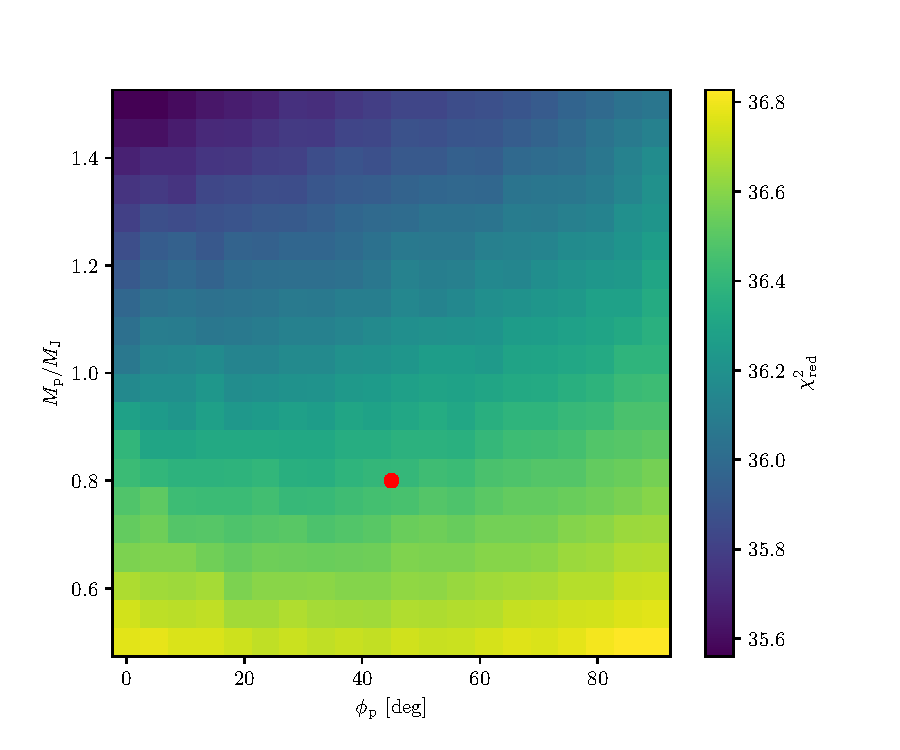
\includegraphics[width = 0.8\textwidth]{figures/planet_mass_az_grid_var.pdf}
    \caption{Grid search in $\chi^2_{\rm red}$ fitting synthetic observations generated with our model. $M_{\rm p}$ and $\phi_{\rm p}$ were both varied around their true values, while all other parameters were set exactly to the values used to generate the synthetic observations. We see that the minimum in $\chi^2_{\rm red}$ once again occurs for the highest mass planet provided, and is not centred on the true values shown by the red dot.}
    \label{fig:planet_grid_search}
\end{figure}

\subsection{Discussion}

The results obtained in Section~\ref{sec:model_model_fit} indicate that our choice of $\chi^2_{\rm red}$ is not well suited to the problem, as it does not find a minimum at the true value even in the case that the model matches the data exactly.
It is likely that this comes down to how the distance between the individual points are calculated.
Say for example we are finding the distance between contours $A$ and $B$.
For some point along $A$ we find the nearest point on $B$ and calculate the distance.
This is done iteratively until every point on $A$ has a distance, and then these distances are summed.
This works well for the case where our contours vary smoothly, that is there is not planet perturbations.
However adding the planet essentially adds ``wiggles'' in the contour, and adding a larger planet adds larger wiggles.
This means that when points along $A$ are looking for the nearest point on $B$, they are more likely to find a closer point just due to the wiggles.
Thus providing larger mass planets results in a lower $\chi^2_{\rm red}$.

This problem could be solved by getting rid of the nearest point search, and instead using some other notion of the distance between the contours. 
For example, the radial distance could be used, or the azimuthal distance.
The problem with either of these approaches is that the iso-velocity contours have a butterfly shape, where they go from a fair fixed azimuthal and varying radius, to a fixed radius but varying azimuth.
A different idea would be to project a line perpendicularly from contour A and find the distance needed to intersect contour B.
This would work fine in the case of the unperturbed background disk, but adding the planet would result in rays projecting in strange directions due to the N-wave shape of the induced kinks \citep{goodman2001,bollati2021a}.
These reasons highlight why we chose the nearest-neighbour search in the first place, and it is not clear how to modify the procedure to do better.

This problem could be avoided completely if we did not have to simultaneously deal with the background disk and the perturbations, since in essence the problem is that the perturbations are being fit to the background.
As already discussed, subtracting a model to remove the background has numerous issues that would prevent the fitting of semi-analytic models.
It would therefore be valuable to extract the perturbations in a way that is model-independent.
This would still provide results that are not conditioned on assuming some model.
In Section~\ref{sec:mirror_residuals} we present preliminary results on developing a method to do this.

We also found that the minimum in $\phi_{\rm p}$ did not seem to correspond to the true value.
This is harder to explain, although close inspection of Figure~\ref{fig:planet_grid_search} shows that actually the minimum in $\phi_{\rm p}$ is approximately centred on the true value if we consider only the row of results with $M_{\rm p} = 0.8 \, \mathrm{M_J}$ (which is the true planet mass value).
This position then seems to shift to smaller $\phi_{\rm p}$ and $M_{\rm p}$ increases.
It is possible that this is due to the relative invariance of spiral shape to rotation, since the radial locations change slowly as the azimuth varies.

\section{Mirror Residuals} \label{sec:mirror_residuals}

Another aspect of \citet{calcino2022} that we would like to build on is the detection of the wake itself.
The method we presented there, of mapping the wake through the peak velocity plot through spatially correlated deviations in nearby iso-velocity contours, relies on a by eye inspection and so is subject to human bias.
By exploiting the symmetry of channel maps, we can instead extract asymmetries in the disk systematically, and produce an ``image'' of the planet wake.

Once the systemic velocity has been subtracted, velocity channel maps have both negative and positive velocity channels, with some spacing in velocity $\Delta v$.
For a perfectly axisymmetric disk, the corresponding curves of iso-velocity on each side of the disk should be symmetric around the semi-major axis.
This can be seen in the middle panel of Figure~\ref{fig:conts_obs_model}, where the blue and red sides of the disk are just the reflection of each other.
Therefore, the velocity channel $v=-200 \, \mathrm{m/s}$ for example, should look the same as the channel $v=+200 \, \mathrm{m/s}$ after an appropriate rotation, if the disk were perfectly axisymmetric.
By associating channels with their symmetric partner, one can therefore subtract one from the other to create residuals that show any asymmetries between one side of the disk to the other.

In reality, the systemic channel of the cube is unlikely to have a velocity of zero, and so the velocity of the negative channels will not line up exactly with those from the positive channels.
To remedy this, we simply linearly interpolated the cube in the velocity direction (that is, we interpolated along the line-profile of each pixel), to obtain interpolated channels such that they could be paired up exactly.
We performed this analysis again on the MAPS $^{12}$CO data of HD~163296 \citep{oberg2021}.
The left panel shows the $v=0.5$ km/s channel, while the middle panel shows the corresponding $v=-0.5$ km/s channel that has been interpolated from the negative velocity channels.
The right panel shows the residuals calculated after subtracting one channel from the other.
This process yields a cube of ``mirror residuals''.

\begin{figure}
    \centering
    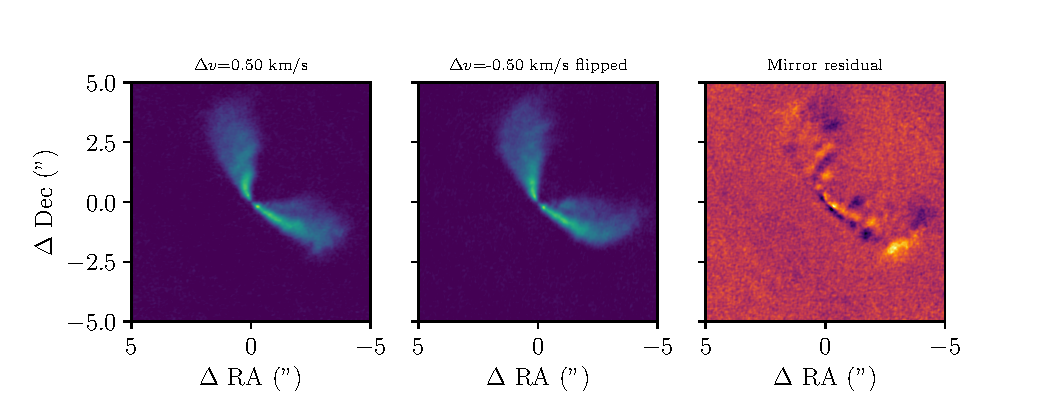
\includegraphics[width = 0.999\textwidth]{figures/channel060jvm.pdf}
    \caption{The left panel shows the $\Delta v = 0.5$ km/s velocity channel taken from the $0.15"$ resolution MAPS observations of HD~163296. The middle panel shows the corresponding $\Delta v = -0.5$ km/s interpolated from the cube. The right panel shows the residuals calculated by subtracting the middle image from the left image. We see that the bottom right velocity kink from \citet{calcino2022} shows up in the residuals as a bright blob.}
    \label{fig:mirror_residuals}
\end{figure}

Collapsing this cube along the velocity axis by taking for each pixel its value in the channel where it is brightest, the so-called peak intensity map or moment-8, yields a map of asymmetries in the disk.
This is shown in Figure~\ref{fig:mirror_M8}.
Two large bright arcs can be seen in the figure.
The bottom-most arc can be identified as the wake from the planet, which we demonstrate by plotting the wake shape projected to the emitting layer as in \citet{calcino2022}.
The other large bright arc does not seem to be associated with the planet wake, and has been previously identified by \citet{teague2021} and \citet{calcino2022}.

\begin{figure}
    \centering
    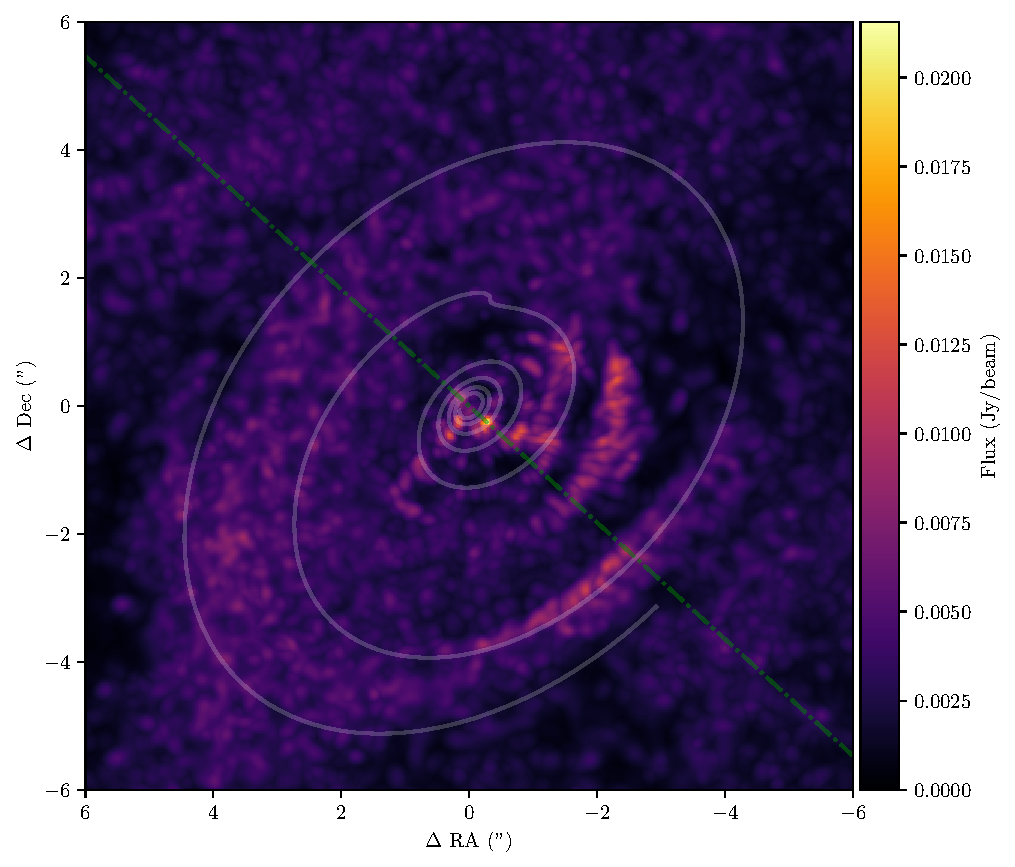
\includegraphics[width = 0.9\textwidth]{figures/mirror_M8.pdf}
    \caption{Peak intensity plot, generated from the mirror residuals of the MAPS $^{12}$CO kinematic observations of HD~163296 \citep{oberg2021}. Plotted also is the shape of the planet wake projected to the emitting layer from \citet{calcino2022}. We clearly see the planet wake as a bright arc in the bottom right of the image. Also identified is a further bright arc not associated with the planet wake, which has also been pointed out by \citet{teague2021} and \citet{calcino2022}. The green dot-dashed line shows the line of symmetry for the plot, since each half of the disk has been used to subtract the other half, it is ambiguous which side of the green line each feature in the map should actually be on.}
    \label{fig:mirror_M8}
\end{figure}

Extracting the perturbations associated with the wake in this way is valuable because unlike other methods \citep{teague2021,teague2022} it is completely model-independent.
It does however come with some important caveats, the first of which is a positional ambiguity in the features identified in the map shown in Figure~\ref{fig:mirror_M8}.
Since the residuals on each half of the disk are found by subtracting the other half, features that show up as positive residuals on one side of the disk will also show up as negative residuals on the other side.
One could obtain the symmetric partner of Figure~\ref{fig:mirror_M8} by taking instead the lowest intensity value in each channel from the mirror residuals cube.
\note{finish section}


%\begin{itemize}
%    \item Describe method, makes use of symmetry
%    \item Present residuals 
%    \item Present peak intensity plot 
%    \item Present peak velocity plot
%    \item Discuss ambiguity
%    \item May be a promising way to make wakes more quantitatively
%    \item Hard to use to extract velocities
%\end{itemize}

%\section{Model-Independent Perturbation Extraction} \label{sec:isovelocity_transform}

%\begin{itemize}
%    \item Describe coordinate transform
%    \item Present example using analytics
%    \item Discuss its model dependence issue 
%    \item Describe how in principal this could be done independently of model, does not assume any background disk model, and does not assume axisymmetry of the disk
%    \item Should be able to extract only the planet perturbations
%\end{itemize}



    \chapter{Conclusion}
    The detection and measurement of protoplanets still embedded in the circumstellar disks they formed from is a vital step in constraining models of planet formation.
A promising method for making such measurements is through identifying kinematics features from perturbing planets in observations of molecular line emission in disks.
In this thesis we have built upon semi-analytic methods for modelling the interaction between the planet and the gas disk, and applied this methods to real observations to constrain potential planets.

In Chapters~\ref{ch:disks} and \ref{ch:planetdisk} were reviewed the relevant physics of both protoplanetary disk structure and planet-disk interactions.
We derived the linear disk response to a small perturbation using WKB methods, and found the the Lindblad resonance locations where a tidally-forcing body excited density waves.
Combining these findings we then used phase arguments to derive the shape of the coherent, one-armed wake that is formed from constructive interference of individual modes.
We then reviewed the work of \citet{goodman2001,rafikov2002a} in developing a semi-analytic framework to calculate the density perturbations along the planet wake, in both the linear and non-linear regimes.
Lastly, we applied this framework to determine the quantities that we must constrain observationally in order to measure planet masses.

In Chapter~\ref{ch:wake_models} we presented our Python package \textsc{wakeflow} for generating semi-analytic models of planet wakes in protoplanetary disks.
The package contains both accuracy and efficiency improvements over previous methods.
The accuracy improvements include a more accurate treatment of the initial conditions used in the non-linear wake evolution, improved matching between the linear and non-linear solutions, and a high-order method for extracting the velocity perturbations.

In Chapter~\ref{ch:HD169_IMLUP} we presented two applications of the models to the detection of protoplanets, in the disks of HD~169142 and IM~Lupi.
We found that the kinematic arc identified in HD~169142 is not well explained by the predominantly radial motions in the planet wake.
In IM~Lupi, we found that a spiral structure could be traced through the peak velocity map, providing evidence of an embedded planet.

Finally, in Chapter~\ref{ch:fitting} we presented preliminary work on the development of a fitting procedure to determine planet masses from kinematic observations.
To do this, we fit iso-velocity contours generated by semi-analytic models to the observed peak velocity map.
We found that this performed reasonably well for fitting just an unperturbed disk, but failed once a planet was added due to complications with how the distances between the curves in the model and observations were calculated.
We then presented a model-independent way of extracting the perturbations present in the kinematics, although it remains unclear how to leverage this to perform fitting of the planet mass.
However, this method does allow for quantitative identification of asymmetric features in the disk such as planet wakes, without needing to assume a background model.

\section{Future Work}

    \bibliographystyle{mnras.bst}
    \bibliography{disks.bib}

\end{document}